\documentclass[aps,floatfix,10pt,amssymb,amsfont,amsmath,superscriptaddress,float,nofootinbib,longbibliography,nobalancelastpage,twocolumn]{revtex4-2}
\usepackage{graphicx} % Required for inserting images
\usepackage{hyperref}
\hypersetup{hidelinks}
\usepackage{braket}
\usepackage{amsfonts}
\usepackage{amssymb}
\usepackage{amsmath}
\usepackage{bbm}
\usepackage{bm}
\usepackage[english]{babel}
\usepackage{amsthm}
\newtheorem{theorem}{Theorem}
\newtheorem{definition}{Definition}
\newtheorem{lemma}{Lemma}
\newtheorem{duplicate}{Theorem}
\newtheorem{corollary}{Corollary}
\newtheorem{remark}{Remark}
\newtheorem*{lemma*}{Lemma}
\usepackage{subfig}
\usepackage{tikz}
\usetikzlibrary{arrows,positioning}
\usetikzlibrary{arrows.meta,backgrounds,calc,fit,positioning,shapes.geometric}
 \usetikzlibrary{quotes}
\usepackage{yquant}
\pgfdeclareshape{yquant-multictrlshape}{
   \inheritsavedanchors[from=yquant-circle]%
   \foreach \anc in {center, north, north east, east, south east, south, south west, west, north west} {%
      \inheritanchor[from=yquant-circle]{\anc}%
   }%
   \inheritanchorborder[from=yquant-circle]%
   \backgroundpath{%
      \pgfpathmoveto{\pgfqpoint{-0.707107\dimexpr\xradius\relax}{-0.707107\dimexpr\yradius\relax}}%
      \pgfpathlineto{\pgfqpoint{0.707107\dimexpr\xradius\relax}{0.707107\dimexpr\yradius\relax}}%
      \pgfpathellipse{\pgfpointorigin}%
                     {\pgfqpoint{\xradius}{0pt}}%
                     {\pgfqpoint{0pt}{\yradius}}%
   }%
   \inheritclippath[from=yquant-circle]%
}

\yquantset{multictrl/.style={every negative control/.style={draw, /yquant/default fill,shape=yquant-multictrlshape,radius=1.05mm}}}
\pgfdeclareshape{yquant-bctrlshape}{
   \inheritsavedanchors[from=yquant-circle]%
   \foreach \anc in {center, north, north east, east, south east, south, south west, west, north west} {%
      \inheritanchor[from=yquant-circle]{\anc}%
   }%
   \inheritanchorborder[from=yquant-circle]%
   \backgroundpath{%
      % Draw the circle
      \pgfpathellipse{\pgfpointorigin}%
                     {\pgfqpoint{\xradius}{0pt}}%
                     {\pgfqpoint{0pt}{\yradius}}%
   }%
   % Add the "b" in the center
   \foregroundpath{%
      \pgftext[center]{\(\scriptstyle b\)}%
   }%
   \inheritclippath[from=yquant-circle]%
}

\yquantset{
  bctrl/.style={
    every control/.style={
      draw,
      /yquant/default fill,
      shape=yquant-bctrlshape,
      radius=1.05mm
    }
  }
}
\date{October 2026}
\begin{document}
\yquantdefinebox{dots}[inner sep=0pt]{$\dots$}

\title{Quantum Metropolis Sampling via Boosted Phase Estimation on Arbitrary Ancilla States}
\author{Oliver O'Brien}
\affiliation{Department of Applied Mathematics and Theoretical Physics, University of Cambridge,\\ Wilberforce Road, Cambridge, CB3 0WA, United Kingdom}
\author{Rakesh Achutha}
\affiliation{Department of Applied Mathematics and Theoretical Physics, University of Cambridge,\\ Wilberforce Road, Cambridge, CB3 0WA, United Kingdom}
\author{Frank Verstraete}
\affiliation{Department of Applied Mathematics and Theoretical Physics, University of Cambridge,\\ Wilberforce Road, Cambridge, CB3 0WA, United Kingdom}
\affiliation{Department of Physics and Astronomy, Ghent University, Krijgslaan 281, 9000 Gent, Belgium}

\begin{abstract}
    We introduce a novel technique for efficiently boosting quantum phase estimation (QPE) using window functions that, unlike existing methods, does not require specially prepared ancilla states. The protocol shifts an energy register by the magnitude of the energy, records the sign of the shift in a single flag qubit, and has exponentially suppressed tails. We prove that the Quantum Metropolis Sampling algorithm constructed using Marriott-Watrous rewinding and our new QPE protocol approximately preserves the Gibbs state and hence, under mixing and contraction assumptions, efficiently prepares Gibbs states. This circumnavigates a no-go theorem proving that the boosted shift-invariant phase estimation step of the original Quantum Metropolis construction is impossible to implement.
\end{abstract}

\maketitle

\section{Introduction}
Sampling thermal (Gibbs) states of physical systems is one of the most credible applications for future fault-tolerant quantum computers. Thermal expectation values are of interest across quantum chemistry, condensed matter physics and high energy physics, and classically they are almost all computed by Markov chain Monte Carlo. For many fermionic or frustrated spin systems this approach runs into the sign problem as the weights are not all positive. As the average sign decays exponentially with system size and inverse temperature, the number of samples necessary to resolve the observable grows exponentially \cite{Troyer_2005}. A quantum computer can directly interact with the state rather than only with a signed decomposition, so it does not encounter the sign problem. The classical computer is attempting to replicate the interference that physics gives for free on a quantum computer.

The original quantum algorithm invented for performing this sampling was the Quantum Metropolis algorithm of Temme et. al. \cite{Temme_2011}. This was a direct quantum analogue of Metropolis-Hastings: propose a random unitary move then accept or reject the move based upon the energy before and after the move. The principal challenge of creating a quantum analogue of the Metropolis-Hastings algorithm was rejecting a move. In the classical setting one can either copy the state before the move or simply undo the move after rejecting, however, in the quantum setting copying the initial state is forbidden by the no-cloning principle and simply reversing the proposed unitary does not undo the disturbance caused by the accept/reject measurement. Temme et. al. \cite{Temme_2011} navigated around these challenges by using a Marriott-Watrous \cite{MarriottWatrous} inspired rewinding procedure to approximately return the system to its previous energy upon rejecting a move.

The rewinding procedure requires a modified quantum phase estimation (QPE) protocol, which coherently encodes an estimate of the system’s energy in an ancilla register. This register is reused without resetting it during rewinding, hence the protocol must work even when the register is not initialised to $\ket{0}$. The original construction therefore required QPE to be ``shift-invariant": starting from a register value $p$ rather than zero simply translates the output by $p$. It also required ``boosting" to suppress the tails of the energy-estimation amplitudes, reducing the weight of estimates far from the true energy. Thus, the original Quantum Metropolis algorithm depended upon a  ``boosted shift-invariant" quantum phase estimation protocol that applied a shift to an ancilla register within a given bound of the true energy (with $\tilde E_j = \frac{N}{2\pi}E_j$ with $N=2^{\eta}$ for an $\eta$ ancilla energy register):
\begin{multline}
  \ket{\psi_j}\ket{p} \;\mapsto\; \sum_{s} \alpha(E_j,s)\,\ket{\psi_j}\ket{p+s},
  \\\alpha(E_j,s) = 0 \ \text{ for } |s-\tilde E_j|_{N} > \mu .
  \label{eq:Boostedshiftinvariantqpe}
\end{multline}
where $\ket{\psi_j}$ is an energy eigenstates with energy $E_j$, $\mu$ is the allowed error in register units, and $|\cdot|_{N}$ measures distance accounting for the register’s wraparound.

Recently the field has been reshaped by a new paradigm based on Davies-generator Lindbladian evolution \cite{chen2023quantumthermalstatepreparation,Kastoryano2014QuantumGS,shtanko2021preparing,chen2021fast,chen2023efficient,rall2023thermal,gilyen2024quantum,ding2025efficient,ding2025end,guo2025designing,chen2025efficient, hahn2026efficient, scandi2026thermalization,leng2026accelerating,rouze2026optimal,lloyd2026quantum,Rouz__2026} which has largely displaced the Metropolis approach in the literature. This current dominance of Lindbaldian samplers is in no small part due to the no-go theorem contained in Appendix H of \cite{chen2023quantumthermalstatepreparation}. This proved it is impossible to implement the ``boosted shift-invariant" quantum phase estimation protocol \eqref{eq:Boostedshiftinvariantqpe} that the original Quantum Metropolis algorithm required.  The original implementation \cite{Temme_2011} suggested taking the median of multiple QPE runs which fails to be ``shift-invariant" as the difference of medians is not necessarily close to the median of the differences. This no-go theorem is widely regarded as closing the book on Quantum Metropolis sampling. 

In this work we restore the Quantum Metropolis algorithm by navigating around this no-go theorem. We introduce a Boosted State-Independent Quantum Phase Estimation (BSI-QPE) protocol which ensures the magnitude of the shift in the ancilla register is close to the true energy with the sign of this shift recorded in an additional flag qubit:
\begin{multline}
  \ket{\psi_j}\ket{p}\ket{f} \;\mapsto\; \sum_{s,f'} \alpha_{f'f}(E_j,s)\,
  \ket{\psi_j}\ket{p+(-1)^{f'}s}\ket{f'},\\
  \qquad \sum_{|s-\tilde E_j|_{N} > \mu} \big|\alpha_{f'f}(E_j,s)\big| = O(e^{-\nu\mu}).
\end{multline}
This protocol is implementable and can fulfill the same role as the previous impossible protocol, with the modification that whenever we previously controlled off the value of the energy register we now must also control off the flag qubit. We carefully account for the non-zero but exponentially suppressed tails of this protocol in our proof work.

Our main contributions are as follows:
\begin{enumerate}
    \item \textbf{Circuit level construction of BSI-QPE} (Section~\ref{section:boostedphaseestimation}): Standard methods  \cite{babbush2018encoding, rendon2022effects, berry2024analyzing, greenaway2024case, patel2026optimal} for boosting QPE require a input ancilla state specially prepared to have amplitudes given by a window function. Here we propose a novel construction which boosts QPE independent of the input ancilla state with the window functions instead being introduced by a controlled single qubit $R_Y$ rotation. We show that unboosted QPE is insufficient for our later proof of approximate quantum detailed balance without a promise that energies are exactly representable in $\eta$ bits. Our novel BSI-QPE protocol is an important invention in its own right, and should have far reaching applications in other quantum algorithms which require coherent phase estimation (e.g. HHL \cite{harrow2009quantum}).
    \item \textbf{Complementary window functions} (Appendix~\ref{section:appendix}): Our construction of BSI-QPE requires a complementary pair of window functions that satisfy $\alpha(x)^2 + \beta(x)^2 =1$ and both have exponentially decaying fourier coefficients. None of the standard  window functions (e.g. DPSS, Kaiser window, Gaussian) are close to satisfying this form. We have found a novel pair of window functions that satisfy these requirements which we demonstrate numerically and prove analytically.
    \item \textbf{Elementary analysis of rewinding} (Section~\ref{section:rejection}): We provide an alternative explanation of the rewinding procedure to the Jordan's-lemma treatment of \cite{Temme_2011} which we find more transparent.
    \item \textbf{Approximate Quantum Detailed Balance Condition} (Section~\ref{section:detailedbalancedef}): We introduce a new branch-wise KMS-inspired detailed balance criteria. This allows us to consider the additive errors introduced by the exponentially suppressed (but non-zero) tails of our BSI-QPE protocol that were neglected in the original treatment \cite{Temme_2011}. We later use this condition to establish that the algorithm approximately preserves the Gibbs state.
    \item \textbf{Approximate Quantum Detailed Balance Proof} (Section~\ref{section:proofmain}): We introduce a novel \textbf{truncate} step to the proof which bounds the additive error due to the non-zero tails of BSI-QPE. We carefully convert the modular norm of the energy approximations to a standard norm \eqref{eq:condJ}-\eqref{eq:kappaclose}. We provide a novel and elegant proof (Lemma~\ref{lemma:summed-history-reversal}) that the measurement outcomes during the rejection procedure can be reversed. Further, we derive an error term \eqref{eq:Wdrifterror} overlooked in \cite{Temme_2011} that is due to the QPE energy register not being exactly returned to $\ket{0}$.
    \item \textbf{Main result} (Theorem~\ref{theorem:main}): Let $\mathcal{E}$ be one  update step of the Quantum Metropolis algorithm run with $\eta$ ancilla qubits in the energy register and a budget of at most $n^*$ rewinding attempts. Under the conditions of Theorem 1, the fixed point $\sigma^*$ of $\mathcal{E}$ is close to the Gibbs state $\sigma_G$ in trace norm $\|\cdot\|_*$:
    \begin{equation}
       \|\sigma_G- \sigma^*\|_* = O\left(\frac{\ell\max\left( n^{*\frac{7}{2}}\sqrt{\frac{\beta\|H\| }{2^{\eta}}}\log^{\frac{9}{2}}n^*,\frac{1}{n^*}\right)}{1-k}\right)
    \end{equation}
    where $k$ is the ergodicity coefficient of $\mathcal{E}^\ell$.
\end{enumerate}
Theorem~\ref{theorem:main} restores the approximate Gibbs-invariance result of the original framework \cite{Temme_2011}, as before this does not directly prove rapid convergence which depends on the mixing properties of $\mathcal{E}$. Proving polynomial time convergence for a general Hamiltonian is likely infeasible as it would allow the solution of QMA-complete problems in polynomial time \cite{kempe2006complexity}. However, under the assumption of strict trace-norm contractivity taken in \cite{Temme_2011} we prove exponentially fast convergence to the fixed point.

Three other routes to Metropolis-type dynamics sidestep shift-invariant phase estimation entirely. Jiang and Irani \cite{jiang2024quantummetropolissamplingweak} replace rewinding with weak measurement and prove that the Gibbs state is an approximate fixed point. Because each iteration moves the state only by $O(\tau^2)$ for a small weak-measurement parameter $\tau$, the number of iterations grows by a polynomial factor. Zhang, Bosse and Cubitt \cite{zhang2023dissipative} instead weakly measure the local terms of the Hamiltonian in sequence with the Gibbs state reached at the stopping time of a conditionally stopped process rather than as the fixed point of a Markov chain. Gilyén et al. \cite{gilyen2024quantum} construct efficiently implementable discrete-time channels that are exactly detailed balanced. They also show how Metropolis-style samplers that estimate energies before and after a jump can be made exactly detailed balanced, implementing rejection with an additional Kraus operator rather than by Marriott–Watrous rewinding. Our guarantees are weaker than those of \cite{gilyen2024quantum}: we obtain approximate rather than exact Gibbs stationarity, and we prove no mixing-time bounds. Our contribution is of a different kind. We show that the original accept/reject-with-rewinding architecture of \cite{Temme_2011}, widely regarded as ruled out, is sound, because it requires a weaker phase-estimation primitive than the one the no-go theorem \cite{chen2023quantumthermalstatepreparation} forbids. We regard these frameworks as complementary, and which is most efficient in practice remains open.

The remainder of the paper is organised as follows. Section~\ref{section:boostedphaseestimation} presents the detailed construction of our Boosted State-Independent Quantum Phase Estimation (BSI-QPE) protocol, including a detailed circuit-level description and error analysis based on window functions (extended by Appendix~\ref{section:appendix}). Section \ref{section:algorithm} describes our modified Quantum Metropolis algorithm incorporating our improved quantum phase estimation; Fig.~\ref{fig:quantum-metropolis-flowchart} provides an complete overview to help guide the reader. Section~\ref{section:why} presents the main theorem of the paper, defines our approximate quantum detailed balance framework, and outlines the four-step proof strategy applied to each branch; the full proofs are given in Appendices~\ref{appendix:Aproof} and \ref{appendix:Bproof}. Finally, Section \ref{section:discussion} discusses the broader implications of our results, the assumptions made, and the outlook for implementing these techniques on near-term or fault-tolerant quantum hardware.


\section{Boosted State-Independent Quantum Phase Estimation}
\label{section:boostedphaseestimation}

Given Hamiltonian $H$ with eigenvectors $\ket{\psi_j}$ such that $H\ket{\psi_j} = E_j \ket{\psi_j}$, quantum phase estimation (QPE) allows one to prepare an ancilla register that approximates $E_j$. Unfortunately, quantum computers have limited precision. As a result, unless the energy can be represented exactly in binary using $\eta$ bits (corresponding to $\eta$ ancilla qubits), the estimation amplitudes have slowly decaying ``fat tails'', leaving weight on estimates far from the true energy \cite{Nielsen_Chuang_2010}.

Often this issue can be mitigated by simply repeating the calculation and taking an average. However, quantum metropolis sampling requires the estimate to be available for later coherent operations, and we must be able to ``rewind" upon rejecting a proposed update. Therefore, we require a coherent method for ``boosting" QPE. 

Standard methods \cite{babbush2018encoding, rendon2022effects, berry2024analyzing, greenaway2024case, patel2026optimal} for coherently boosting QPE rely upon choosing specific input ancillary states\footnote{Coherent boosting without a window state is also possible via the medians trick \cite{nagaj2009fast} used in \cite{Temme_2011}, or via an amplifying polynomial implemented by singular value transformation \cite{rall2021faster}. Both, however, assume a fresh ancilla register in $\ket{0}$, so neither is ``state-independent" or ``shift-invariant".}. They perform QPE using ancillas initialised to the state $\frac{1}{\sqrt{N}}\sum_x \alpha(x) \ket{x}$ for some window function $\alpha(x)$ instead of the standard uniform superposition. After performing QPE upon eigenstate $\ket{\psi_j}$ the following state is produced:
\begin{equation}
   \frac{1}{N} \sum_x \sum_k e^{\frac{2 \pi i}{N}x(k-E_j)} \alpha(x)\ket{k}\ket{\psi_j}
\end{equation}
which can be rewritten as:
\begin{equation}
    \sum_k \hat\alpha(k-E_j) \ket{k}\ket{\psi_j}
\end{equation}
where $\hat \alpha(k)$ is the discrete Fourier transform of $\alpha(x)$. By choosing $\alpha$ to be a window function one can ensure that $\hat \alpha$ is narrowly peaked, thus QPE is boosted. Unfortunately, this is not sufficient for the quantum Metropolis algorithm as we require the QPE to be independent of the ancillary state, as we must reuse the same ancillas throughout the rewinding process. 

Our BSI-QPE protocol achieves coherent boosting without requiring a specially prepared input ancilla state. It adds or subtracts an energy estimate from the existing register value, recording the direction in a flag qubit, with exponentially suppressed estimation tails as shown in Fig.~\ref{fig:Gshift}.


\begin{figure*}
\centering
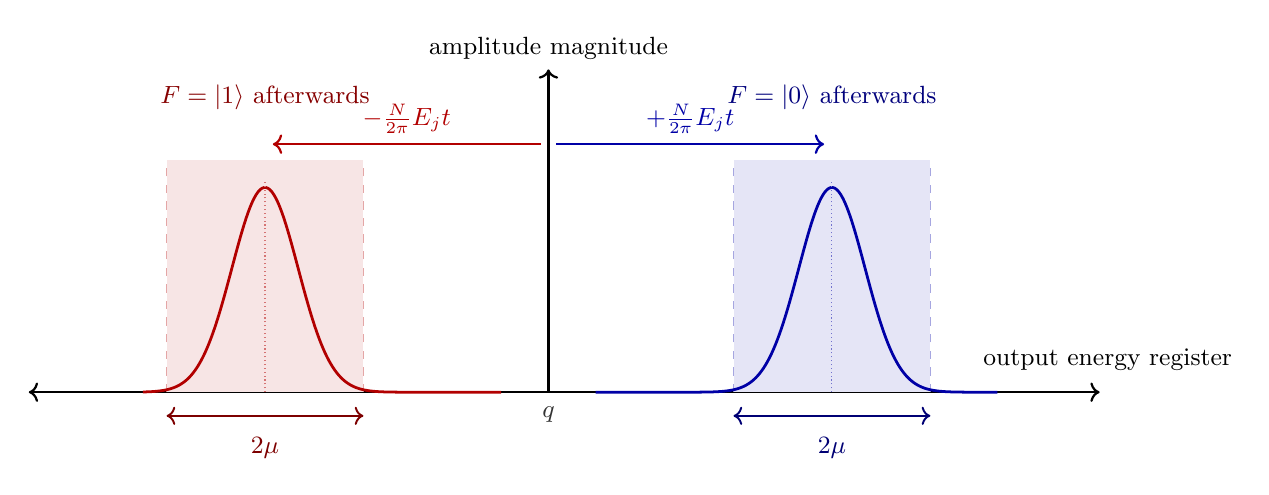
\begin{tikzpicture}
 
% ---- parameters -------------------------------------------------
\def\qq{5.6}        % input value q
\def\dd{3.6}        % shift  (2^eta/2pi) E_j t
\def\sg{0.42}       % peak width
\def\mw{1.25}       % half-window mu
\def\hh{2.6}        % peak height
\pgfmathsetmacro{\cL}{\qq-\dd}
\pgfmathsetmacro{\cR}{\qq+\dd}
 
% ---- axes -------------------------------------------------------
\draw[<->,thick] (-1,0) -- (12.6,0);
\node[anchor=west,font=\small] at (11.0,0.42) {output energy register};
% \draw[->,thick] (0.4,-0.05) -- (0.4,4.1) node[above,font=\small] {amplitude};
 
% ---- input value q ---------------------------------------------
% \draw[->, thick] (\qq,0) -- (\qq,4.1);
\node[gray!40!black,below,font=\small] at (\qq,-0.06) {$q$};
\draw[->,thick] (\qq,0) -- (\qq,4.1) node[above,font=\small] {amplitude magnitude};

 
% ---- one output branch ------------------------------------------
% #1 centre  #2 colour  #3 F-label  #4 centre label
\newcommand{\branch}[4]{%
  \fill[#2!10] (#1-\mw,0) rectangle (#1+\mw,2.95);
  \draw[#2!35,dashed] (#1-\mw,0) -- (#1-\mw,2.95);
  \draw[#2!35,dashed] (#1+\mw,0) -- (#1+\mw,2.95);
  \begin{scope}
    \clip (0.45,-0.05) rectangle (11.3,4.0);
    \draw[#2,line width=1pt] plot[domain=#1-3.0:#1+3.0,samples=240,smooth]
        (\x,{\hh*exp(-(\x-#1)*(\x-#1)/(2*\sg*\sg))});
  \end{scope}
  \draw[#2!55,densely dotted] (#1,0) -- (#1,\hh+0.1);
  \node[#2!75!black,font=\small] at (#1,3.75) {#3};
  \draw[<->,#2!70!black,line width=0.7pt]
        (#1-\mw,-0.3) -- (#1+\mw,-0.3) node[midway,below=4pt,font=\small] {$2\mu$};
  % \node[#2!75!black,font=\small] at (#1,-1.5) {#4};
}
 
\branch{\cL}{red!70!black}{$F=\ket{1}$ afterwards}{$q-\frac{N}{2\pi}E_j t$}
\branch{\cR}{blue!65!black}{$F=\ket{0}$ afterwards}{$q+\frac{N}{2\pi}E_j t$}
 
% ---- shift arrows ----------------------------------------------
\draw[<-,thick,red!70!black]  (\cL+0.1,3.15) -- (\qq-0.1,3.15)
      node[midway,above,font=\small] {$-\frac{N}{2\pi}E_j t$};
\draw[->,thick,blue!65!black] (\qq+0.1,3.15) -- (\cR-0.1,3.15)
      node[midway,above,font=\small] {$+\frac{N}{2\pi}E_j t$};
 
% ---- tail annotation -------------------------------------------
% \node[gray!55!black,align=center,font=\scriptsize] at (\qq,1.15)
%       {exponentially\\ suppressed tails};
% \draw[gray!55!black,->,shorten >=2pt] (\qq-1.0,0.95) -- (\cL+1.65,0.13);
% \draw[gray!55!black,->,shorten >=2pt] (\qq+1.0,0.95) -- (\cR-1.65,0.13);
 
\end{tikzpicture}
\caption{Action of BSI-QPE on an energy eigenstate $\ket{\psi_j}$ with the energy register initially holding $q$. The output has two branches centered on $q\pm\frac{N}{2\pi}E_jt$, distinguished by the output flag qubit $F$. The window functions concentrate the amplitudes around these centres and suppress the tails exponentially. The exact shape of the amplitude distribution depends upon the value of $F$ before the action of BSI-QPE, however it is of little consequence as they both have exponentially decaying tails.}
\label{fig:Gshift}
\end{figure*}

Our construction uses two window functions $\alpha(x)$ and $\beta(x) = \sqrt{1-\alpha(x)^2}$ (for $x\in\{0,1,\ldots,N-1\}$) which are both narrowly peaked in the Fourier domain. We introduce these windows via the following multi-controlled single-qubit rotation:
\begin{equation}
   CR_Y = \sum_k \ket{k}\bra{k}\otimes \begin{pmatrix}
        \alpha(k)& \beta(k)\\
        -\beta(k)& \alpha(k)
    \end{pmatrix}
\end{equation}

We also require the following time evolution gadget which is constructed as shown in Fig~\ref{fig:CRZ}:
\begin{equation}
    CR_Z =\sum_{j,k}\ket{\psi_j}\bra{\psi_j}\otimes\ket{k}\bra{k} \otimes \begin{pmatrix}
        e^{\frac{iE_jkt}{2}}&0\\
        0 & e^{-\frac{iE_jkt}{2}}
    \end{pmatrix}
\end{equation}
\begin{figure*}
\[
\vcenter{\hbox{
\resizebox{!}{2.5cm}{
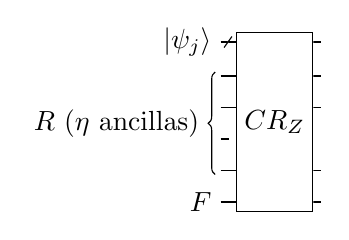
\begin{tikzpicture}
\begin{yquant*}
qubit {$\ket{\psi_j}$} s;

init {$R$ ($\eta$ ancillas)} (a[0,1],ellipsis, aend);
slash s;
hspace {0.1cm} -;
discard ellipsis;
% qubit {} aend;
qubit {$F$} f;
box {$CR_Z$} (s,a,ellipsis, aend, f);

% text {$\ket{0}$} f;
\end{yquant*}
\end{tikzpicture}}}}
=
\vcenter{\hbox{
\resizebox{!}{2.5cm}{
    \begin{tikzpicture}
\begin{yquant*}
qubit {$\ket{\psi_j}$} s;

init {$R$} (a[0,1],ellipsis, aend);
discard ellipsis;
% qubit {} aend;
qubit {$F$} f;
slash s;
hspace {0.1cm} -;

box {$U^{\dagger 2^0}$} (s) | a[0], f;
box {$U^{\dagger 2^1}$} (s) | a[1], f;
hspace {0mm} -;
dots ellipsis;

box {$U^{\dagger 2^{\eta-1}}$} (s) | aend[0], f;
box {$U^{2^0}$} (s) | a[0]~ f;
box {$U^{ 2^1}$} (s) | a[1]~ f;
hspace {0mm} -;
dots ellipsis;

box {$U^{ 2^{\eta-1}}$} (s) | aend[0]~ f;
\end{yquant*}
\end{tikzpicture}}}}
\]
\caption{Quantum circuit for implementing an $Z$ rotation on an ancilla qubit that is dependent upon the energy of the system. The unitary $U=e^{\frac{iHt}{2}}$ is implemented through some quantum time evolution algorithm (e.g. trotterisation \cite{lloyd1996universal}, qubitization \cite{Low2019hamiltonian}) up to an operator norm error of $\epsilon^T_t$. Throughout this work we assume  $\epsilon^T_t$ is negligible, and use perfect quantum time evolution in our error analysis.}
    \label{fig:CRZ}
\end{figure*}
Conditioned on the system being in $\ket{\psi_j}$ and the ancilla register in $\ket{k}$,
both gadgets act on the flag qubit $F$ as single-qubit rotations: $CR_Y$ applies
$R_Y[2\arccos\alpha(k)]$ and $CR_Z$ applies $R_Z[E_jkt]$, where throughout we use the convention
\begin{align}
R_Z(\phi) = \begin{pmatrix} e^{i\phi/2} & 0\\ 0 & e^{-i\phi/2}\end{pmatrix}\\
R_Y(\theta) = \begin{pmatrix} \cos\frac{\theta}{2} & \sin\frac{\theta}{2}\\ -\sin\frac{\theta}{2} & \cos\frac{\theta}{2}\end{pmatrix}
\end{align}
\begin{figure*}
\[
\vcenter{\hbox{
\resizebox{!}{2.5cm}{
\begin{tikzpicture}
    \begin{yquant*}
qubit {$\ket{\psi_j}$} s;

init {$R$ ($\eta$ ancillas)} (a[0,1],ellipsis, aend);
slash s;
% hspace {0.1cm} -;
discard ellipsis;
% qubit {} aend;
qubit {$F$} f;
dots ellipsis;

box {BSI-\\QPE} (s,a,ellipsis, aend, f);

% text {$\ket{0}$} f;
\end{yquant*}
\end{tikzpicture} }}}
=
\vcenter{\hbox{
\resizebox{!}{3cm}{
\begin{tikzpicture}
    \begin{yquant*}
qubit {$\ket{\psi_j}$} s;

init {$R$} (a[0,1],ellipsis, aend);
slash s;
discard ellipsis;
% qubit {} aend;
qubit {$F$} f;
dots ellipsis;
box {QFT} (a,ellipsis, aend);

[this subcircuit box style={dashed, "$R_Z[E_jt(k-k')]$"}]
subcircuit {
qubit {} s;
qubit {} a[2];
nobit ellipsis;
qubit {} aend;
qubit {} f;

% dots ellipsis;
box {$CR_Z$} (s,a,ellipsis, aend, f);

x aend[0];
dots ellipsis;
box {$CR_Z^{\dagger}$} (s,a,ellipsis, aend, f);
x aend[0];
dots ellipsis;
} (s,a,ellipsis, aend, f);

box {$CR_Y$} (a,ellipsis, aend, f);

[this subcircuit box style={dashed, "$R_Z[E_jt(k+k'-N)]$"}]
subcircuit {
qubit {} s;
qubit {} a[2];
nobit ellipsis;
qubit {} aend;
qubit {} f;

box {$CR_Z$} (s,a,ellipsis, aend, f);
x aend[0];
dots ellipsis;
box {$CR_Z$} (s,a,ellipsis, aend, f);
x aend[0];
dots ellipsis;
box {$U^{\dagger N}$} (s) ~ f;
box {$U^{N}$} (s) | f;
} (s,a,ellipsis, aend, f);

box {iQFT} (a,ellipsis, aend);

% text {$\ket{0}$} f;
\end{yquant*}
\end{tikzpicture} }}}
\]

\caption{Quantum circuit implementing boosted state-independent quantum phase estimation (BSI-QPE). We highlight how the combinations of $CR_Z$ and $X$ gates operators correspond to the single qubit $R_Z$ given in Eq.~\ref{eq:euler} with $k$ being the value stored in the $\eta$ ancillas and $k' = k + \frac{N}{2} \mod N$}
\label{fig:circuit}
\end{figure*}
\begin{figure*}
\begin{tikzpicture}
    \begin{yquant*}
qubit {$\ket{\psi_j}$} s;

init {$\eta$ ancillas} (a[0,1],ellipsis, aend);
slash s;
discard ellipsis;
% qubit {} aend;
dots ellipsis;
box {QFT} (a,ellipsis, aend);

box {$U^{ 2^1}$} (s) | a[0];
box {$U^{ 2^2}$} (s) | a[1];
hspace {0mm} -;
dots ellipsis;

box {$U^{ N}$} (s) | aend[0];
box {$U^{\dagger N}$} (s);
box {iQFT} (a,ellipsis, aend);

% text {$\ket{0}$} f;
\end{yquant*}
\end{tikzpicture} 

\caption{Quantum circuit implementing unboosted state-independent QPE with $U=e^{\frac{iHt}{2}}$, equivalent to choosing $\alpha(x)=1$ for BSI-QPE and acting upon $\ket{0}_F$. This slightly differs from the standard formulation of QPE \cite{Nielsen_Chuang_2010} by beginning with $QFT$ rather than $H^{\otimes \eta}$ and the addition of $U^{\dagger N}$ at the end. }
\label{fig:standard_qpe}
\end{figure*}
\begin{widetext}
BSI-QPE is built from the $R_ZR_YR_Z$ (Euler) decomposition of a single-qubit unitary~\cite{Nielsen_Chuang_2010}, which in the convention above reads
\begin{equation}
\label{eq:euler}
R_Z(\phi_1)R_Y(\theta)R_Z(\phi_2) = \begin{pmatrix}
\cos\frac{\theta}{2}\,e^{i(\phi_1+\phi_2)/2} & \sin\frac{\theta}{2}\,e^{i(\phi_1-\phi_2)/2}\\
-\sin\frac{\theta}{2}\,e^{-i(\phi_1-\phi_2)/2} & \cos\frac{\theta}{2}\,e^{-i(\phi_1+\phi_2)/2}
\end{pmatrix}.
\end{equation}
The circuit in Fig.~\ref{fig:circuit} implements this with angles that depend on the ancilla value $k$. The $X$ gates on the last ancilla qubit map $k\to k' = k+\frac{N}{2} \bmod N$, so the first dashed block implements $R_Z[E_jt(k-k')]$ and the second implements $R_Z[E_jt(k+k'-N)]$, where the $-N$ comes from the $F$-controlled $U^{\pm N}$. Substituting
\begin{equation}
\label{eq:angles}
\theta = 2\arccos\alpha(k),\qquad \phi_1 = E_jt(k+k'-N),\qquad \phi_2 = E_jt(k-k')
\end{equation}
into Eq.~\eqref{eq:euler}, and using $\cos\frac{\theta}{2}=\alpha(k)$, $\sin\frac{\theta}{2}=\beta(k)$, gives
\begin{equation}
\begin{pmatrix}
\alpha(k)e^{iE_jtk}e^{-\frac{iE_jtN}{2}} & \beta(k)e^{iE_jt k'}e^{-\frac{iE_jtN}{2}}\\
-\beta(k)e^{-iE_jt k'}e^{\frac{iE_jtN}{2}} & \alpha(k)e^{-iE_jtk}e^{\frac{iE_jtN}{2}}
\end{pmatrix}.
\end{equation}
Hence, summing over $k$ and the QFTs, we get the following operation:
\begin{multline}
        \text{BSI-QPE} = \frac{1}{N}\sum_j\sum_{p,q,k} \begin{pmatrix}
        \alpha(k)e^{iE_jtk}e^{-\frac{iE_jtN}{2}} && \beta(k)e^{iE_jt[(k+\frac{N}{2})\text{mod} N]}e^{-\frac{iE_jtN}{2}}\\
        -\beta (k)e^{-iE_jt[(k+\frac{N}{2})\text{mod} N]}e^{\frac{iE_jtN}{2}} && \alpha(k)e^{-iE_jtk}e^{\frac{iE_jtN}{2}}
    \end{pmatrix}e^{\frac{2\pi i}{N}k(q-p)} \\\otimes\ket{p}\bra{q}\otimes\ket{\psi_j}\bra{\psi_j}
\end{multline}
This can be simplified to:
\begin{equation}
    \text{BSI-QPE} = \sum_j\sum_{p,q} \begin{pmatrix}
        (-1)^{q-p}\hat\alpha(q-p+\frac{N}{2\pi}E_jt) && \hat\beta(q-p+\frac{N}{2\pi}E_jt)\\
        -\hat\beta (q-p-\frac{N}{2\pi}E_jt) && (-1)^{q-p}\hat\alpha(q-p-\frac{N}{2\pi}E_jt)
    \end{pmatrix}\otimes\ket{p}\bra{q}\otimes\ket{\psi_j}\bra{\psi_j}
\end{equation}
% \begin{multline}
%   \sum_j \sum^{N}_{p,q} \hat \alpha(p - q - \frac{N t}{2\pi}E_j)\ket{0}\bra{0} \otimes\ket{p}\bra{q} \otimes \ket{\psi_j} \bra{\psi_j}\\
%   + \ket{0}\bra{0} \otimes\bm{\varepsilon}^T_{kt}
% \end{multline}
where $\hat \alpha$ is the discrete Fourier transform of $\alpha$ as given by:
\begin{equation}
   \hat\alpha(x) =\frac{1}{N}\sum_{k=-\frac{N}{2}}^{\frac{N}{2}-1} \alpha(k+\frac{N}{2})e^{\frac{2\pi i}{N}xk}
\end{equation}
and $\hat \beta$ is the discrete Fourier transform of $\beta$ given by:
\begin{equation}
    \hat\beta(x) =\frac{1}{N}\sum_{k=-\frac{N}{2}}^{\frac{N}{2}-1} \beta(k)e^{\frac{2\pi i}{N}kx}
\end{equation}
 where $\beta(k)$ is extended by $\beta(k) = \beta(k \mod N)$. 
 \begin{remark}[Why the Fourier transforms use different origins]
     The definition of $\hat\alpha$ shifts the window $\alpha$ by half a period, whereas the definition of $\hat\beta$ does not. This allows each window to be small at the boundaries of its own Fourier summation interval. Using the same origin for both would prevent this, because $\alpha^2+\beta^2=1$. For off-grid energies, the resulting boundary mismatch would introduce slowly decaying tails. The different origins are therefore essential to obtaining exponential tail suppression for both branches.
 \end{remark}
Throughout the rest of this work, we will use the following notational shorthand: 
\begin{equation}
    G_j^{pq} = \begin{pmatrix}
        (-1)^{q-p}\hat\alpha(q-p+\frac{N}{2\pi}E_jt) && \hat\beta(q-p+\frac{N}{2\pi}E_jt)\\
        -\hat\beta (q-p-\frac{N}{2\pi}E_jt) && (-1)^{q-p}\hat\alpha(q-p-\frac{N}{2\pi}E_jt)
    \end{pmatrix}
\end{equation}
This shows that BSI-QPE shifts the energy-index register by approximately $\frac{N}{2\pi}E_jt$, in a direction given by the qubit $F$ after the application as demonstrated by Fig.~\ref{fig:Gshift}. 

\end{widetext}
There are many potential candidates for window functions $\alpha(x)$ and $\beta(x)$. In this work we choose to work with $\alpha(x) = \text{sech}( r\cos^{2b} \frac{\pi x}{N})$ and $\beta(x) = \text{tanh}(r \cos^{2b} \frac{\pi x}{N})$. These can both be shown to have discrete Fourier transforms which decay exponentially fast as we discuss in Appendix~\ref{section:appendix}:
\begin{equation}
    |\hat \alpha(k)|,|\hat \beta(k)| = O\left( \frac{1}{\nu}e^{-\nu |k|}\right)
    \label{eq:scaling}
\end{equation}
where $\nu = \frac{1}{2b}$. Hence we can write:
\begin{equation}
    \hat\alpha(k) = \tilde\alpha(k) + \Delta_{\alpha}(k) \>\>\>\>\>\>\hat\beta(k) = \tilde\beta(k) + \Delta_{\beta}(k)
    \label{eq:decomposealpha}
\end{equation}
where:
\begin{align}
    \tilde\alpha(k) &= \hat\alpha(k)\mathbbm{1}(|k|_{N}\leq \mu)\\
    \tilde\beta(k) &= \hat\beta(k)\mathbbm{1}(|k|_{N}\leq \mu)
    \label{eq:decomposealpha2}
\end{align}  and
\begin{equation}
    \sum_k|\Delta_\alpha(k)|,\sum_k|\Delta_\beta(k)|\leq \epsilon_{\Delta}
    \label{eq:decomposealpha3}
\end{equation} where $\epsilon_{\Delta} = O(\frac{1}{\nu}e^{-\nu \mu})$ and $|x|_N = \min(x \mod N,- x\mod N)$ is the modular norm value of $x$.

\begin{lemma}[Band-limited BSI-QPE]
\label{lemma:0}
    Define $\widetilde{\text{BSI-QPE}}$ as given by:
    \begin{equation}
       \widetilde{\text{BSI-QPE}}= \sum_j \sum_{p,q} \tilde G^{pq}_j \otimes \ket{p}\bra{q} \otimes \ket{\psi_j}\bra{\psi_j}
    \end{equation}
    where 
    \begin{equation}
        \tilde G^{pq}_j = \left(\begin{smallmatrix}
        (-1)^{q-p}\tilde\alpha(q-p+\frac{N}{2\pi}E_jt) && \tilde\beta(q-p+\frac{N}{2\pi}E_jt)\\
        -\tilde\beta (q-p-\frac{N}{2\pi}E_jt) && (-1)^{q-p}\tilde\alpha(q-p-\frac{N}{2\pi}E_jt)
    \end{smallmatrix}\right)
    \end{equation}
    Then,  
    \begin{equation}
        \|\widetilde{\text{BSI-QPE}}-\text{BSI-QPE}\| \leq 2\epsilon_{\Delta}
    \end{equation}
\end{lemma}
Proof is given in Appendix~\ref{section:appendixTrunc}. This shows that our BSI-QPE protocol is very close in operator norm to a fully band-limited BSI-QPE.

\begin{remark}[Why boosting is necessary]
Instead one could attempt to use unboosted state-independent QPE. This would correspond to choosing $\alpha(x)=1$, which simplifies Fig.~\ref{fig:circuit} to Fig.~\ref{fig:standard_qpe}. As this effectively acts as a rectangular window function, $|\hat\alpha(k)| = O(\frac{1}{k})$ for off-grid $k$, so $\epsilon_{\Delta} = O(\log \frac{N}{\mu})$ (compared to $\epsilon_{\Delta} = O(2^{-\nu \mu})$ for BSI-QPE). This bound exceeds $1$ and so unboosted state-independent QPE is insufficient for Quantum Metropolis sampling without the promise of energies exactly represented in $\eta$ bits.
\end{remark}
\medskip
\noindent\fbox{%
\begin{minipage}{\dimexpr\columnwidth-2\fboxsep-2\fboxrule\relax}
\textbf{Summary of BSI-QPE}

BSI-QPE shifts the value stored in the energy register by approximately the magnitude of the system's energy, with the sign of the shift recorded in the flag qubit $F$. Hence, for an $\eta$-qubit register initially holding $q$ the output amplitudes are concentrated around
\begin{equation*}
\begin{aligned}
q+\frac{N}{2\pi}E_jt
    &\quad\text{for }F=\ket{0},\\
q-\frac{N}{2\pi}E_jt
    &\quad\text{for }F=\ket{1}.
\end{aligned}
\end{equation*}
where the arithmetic is modulo $N$. Figure~\ref{fig:Gshift} illustrates this action.\\

Using the window functions constructed above, both branches have exponentially suppressed tails. Changing $q$ simply translates the output, and no specially prepared initial state of the energy register or flag qubit is required. The energy eigenstate $\ket{\psi_j}$ is unchanged. 
\end{minipage}%
}
\medskip


\section{Algorithm}
\label{section:algorithm}
Quantum metropolis is heavily inspired by the classical metropolis-hastings algorithm. The principal idea is to apply a randomly chosen update to the current state then accept/reject this update with a probability given by a function ($\tilde{f}_{E_aE_b}=\min(1, e^{-\beta(E_b-E_a)})$) of the energy before $(E_a)$ and after $(E_b)$ the update. This update process is repeated many times with the system quickly converging to equilibrium. To replicate this on a quantum computer we need to be able to: measure the energy of a state (Section~\ref{section:energymeasurement}), apply some update (Section~\ref{section:update}), accept/reject an update with the correct probability (Section~\ref{section:acceptprob}) and ``undo" an update upon deciding to reject it (Section~\ref{section:rejection}). Figure~\ref{fig:quantum-metropolis-flowchart} illustrates this full algorithm for a single update.


Throughout one full update, let $R$ denote the $\eta$-qubit BSI-QPE energy-index register and qubit $F$ the additional qubit on which the $G_j^{pq}$ act. At the start of the update, $R$ is initialised to $\ket{0}$ whilst $F$ is in the maximally mixed state (by classically choosing a random initial state $\ket{0}$ or $\ket{1}$) and the qubit $M$ on which the acceptance rotation $W_{abde}$ acts is initialized in $\ket{0}$. 
\begin{figure*}[t]
  \centering
  % Quantum Metropolis update: portrait, algorithm-at-a-glance flowchart.
% Required in the parent document:
%   \usepackage{amsmath,amssymb,tikz}
%   \usetikzlibrary{arrows.meta,backgrounds,fit,shapes.geometric}
%
% When a referenced label exists, \qmsectionref prints its section number.
% In a standalone build it falls back to the subsection title.
\makeatletter
\providecommand{\qmsectionref}[2]{%
  \ifcsname r@#1\endcsname Sec.~\ref{#1}\else\S~#2\fi}
\makeatother

\definecolor{qmNavy}{HTML}{17324D}
\definecolor{qmBlue}{HTML}{2F6B9A}
\definecolor{qmBlueFill}{HTML}{EAF3F8}
\definecolor{qmOrange}{HTML}{C66A1B}
\definecolor{qmOrangeFill}{HTML}{FFF2E6}
\definecolor{qmPurple}{HTML}{725A9A}
\definecolor{qmPurpleFill}{HTML}{F1EDF7}
\definecolor{qmGreen}{HTML}{2F7D5C}
\definecolor{qmGreenFill}{HTML}{E8F4EE}
\definecolor{qmRed}{HTML}{A33A3A}
\definecolor{qmRedFill}{HTML}{F9EAEA}
\definecolor{qmGray}{HTML}{52606D}
\definecolor{qmGrayFill}{HTML}{F4F6F8}

\begin{tikzpicture}[scale=.94,transform shape,
  font=\sffamily\footnotesize,
  line cap=round,
  line join=round,
  >={Stealth[length=2.4mm,width=1.7mm]},
  flow/.style={->,draw=qmNavy,line width=.9pt},
  process/.style={
    draw=qmNavy,fill=white,rounded corners=2.5pt,
    line width=.8pt,minimum height=10.5mm,minimum width=23mm,
    align=center,inner xsep=5pt,inner ysep=3.5pt
  },
  quantum/.style={process,draw=qmPurple,fill=qmPurpleFill},
  update/.style={process,draw=qmBlue,fill=qmBlueFill},
  test/.style={
    diamond,aspect=1.8,draw=qmNavy,fill=white,
    line width=.85pt,minimum width=20mm,minimum height=13mm,
    align=center,inner sep=1.5pt
  },
  state/.style={
    ellipse,draw=qmNavy,fill=qmGrayFill,line width=.85pt,
    minimum width=21mm,minimum height=10mm,align=center
  },
  accepted/.style={state,draw=qmGreen,fill=qmGreenFill},
  failed/.style={state,draw=qmRed,fill=qmRedFill},
  branchlabel/.style={
    font=\sffamily\scriptsize,fill=white,inner sep=1.5pt
  },
  stepref/.style={font=\sffamily\tiny,text=qmGray},
  note/.style={font=\sffamily\scriptsize,text=qmGray,align=center},
  legend/.style={
    draw=qmGray!55,fill=qmGrayFill,rounded corners=3pt,
    line width=.65pt,align=left,inner sep=6pt,
    text width=55mm,font=\sffamily\scriptsize
  }
]

% Main vertical spine -------------------------------------------------------
\node[state] (rho) at (0,0) {$\rho$};

\node[quantum] (energy) at (0,-1.65) {
  $E_{ae}$\\[-1pt]
  \scriptsize measure energy; record $(a,e)$\\[-1pt]
  \tiny\color{qmGray}\qmsectionref{section:energymeasurement}{Measure the energy}
};

\node[update] (chooseC) at (0,-3.35) {
  pick $C\sim\mathrm d\mu(C)$ and apply $C$\\[-1pt]
  \tiny\color{qmGray}\qmsectionref{section:update}{Update}
};

\node[quantum] (qpe) at (0,-5.05) {
  BSI--QPE\\[-1pt]
  \scriptsize prepare $(b,d)$ in the persistent $R,F$ register\\[-1pt]
  \tiny\color{qmGray}\qmsectionref{section:boostedphaseestimation}{Boosted phase estimation}
};

\node[quantum] (rotate) at (0,-6.75) {
  $W_{abde}$ on $M$\\[-1pt]
  \scriptsize acceptance rotation\\[-1pt]
  \tiny\color{qmGray}\qmsectionref{section:acceptprob}{Accept or Reject}
};

\node[test] (sdecision) at (0,-8.55) {
  measure $M$\\[-1pt]$s\ ?$
};

\draw[flow] (rho) -- (energy);
\draw[flow] (energy) -- (chooseC);
\draw[flow] (chooseC) -- (qpe);
\draw[flow] (qpe) -- (rotate);
\draw[flow] (rotate) -- (sdecision);

% Accept branch: spacious right-hand column --------------------------------
\node[quantum] (measurebd) at (4.25,-8.55) {
  measure $R,F$\\[-1pt]
  \scriptsize record final $(b,d)$\\[-1pt]
  \tiny\color{qmGray}\qmsectionref{section:acceptprob}{Accept or Reject}
};
\node[quantum] (unqpeA) at (4.25,-10.25) {BSI--QPE$^{\dagger}$};
\node[accepted] (rhoA) at (4.25,-11.80) {$\rho_{\mathrm{accept}}$};

\draw[flow,draw=qmGreen]
  (sdecision.east) -- node[branchlabel,above] {$s=1$} (measurebd.west);
\draw[flow,draw=qmGreen] (measurebd) -- (unqpeA);
\draw[flow,draw=qmGreen] (unqpeA) -- (rhoA);

% Reject branch: spacious left-hand column ---------------------------------
\node[quantum] (unrotate) at (-4.25,-8.55) {
  $W_{abde}$ on $M$\\[-1pt]
  \scriptsize uncompute rotation
};
\node[quantum] (unqpeR) at (-4.25,-10.25) {BSI--QPE$^{\dagger}$};
\node[update] (undoc) at (-4.25,-11.80) {
  apply $C^{\dagger}$\\[-1pt]
  \tiny\color{qmGray}\qmsectionref{section:acceptprob}{Accept or Reject}
};

\draw[flow,draw=qmOrange]
  (sdecision.west) -- node[branchlabel,above] {$s=0$} (unrotate.east);
\draw[flow,draw=qmOrange] (unrotate) -- (unqpeR);
\draw[flow,draw=qmOrange] (unqpeR) -- (undoc);

% Overlapping boxes explicitly identify the two maps. Their line patterns
% remain distinct when the paper is printed in grayscale.
\begin{pgfonlayer}{background}
  \node[
    draw=qmBlue,fill=qmBlueFill,fill opacity=.20,
    densely dashed,line width=1.05pt,rounded corners=5pt,
    fit={(chooseC) (qpe) (rotate) (sdecision) (measurebd) (unqpeA) (rhoA)},
    inner sep=8pt
  ] (lbox) {};
  \node[
    draw=qmOrange,fill=qmOrangeFill,fill opacity=.18,
    dash pattern=on 5pt off 2pt on 1pt off 2pt,
    line width=1.05pt,rounded corners=5pt,
    fit={(chooseC) (qpe) (rotate) (sdecision) (unrotate) (unqpeR) (undoc)},
    inner sep=8pt
  ] (qbox) {};
\end{pgfonlayer}

\node[
  anchor=north east,font=\sffamily\bfseries\small,text=qmBlue,
  fill=white,inner sep=1.5pt
] at (5.18,-12.70) {$L^{ade}_{b}$: accepted-update map};
\node[
  anchor=south west,font=\sffamily\bfseries\small,text=qmOrange,
  fill=white,inner sep=1.5pt
] at (qbox.north west) {$Q^{ae}_{0}$: initial reject projector};

% Rejection / Marriott--Watrous rewind routine ------------------------------
\node[process,fill=qmGrayFill,minimum width=14mm] (init) at (-5.90,-15.05)
  {$k\leftarrow0$};
\node[quantum] (ptest) at (-3.40,-15.05) {
  measure $P^{ae}_{s}$\\[-1pt]
  \scriptsize initial-energy test
};
\node[test] (pdecision) at (-.35,-15.05) {$s\ ?$};
\node[test] (limit) at (2.45,-15.05) {$k<n^{\star}$?};
\node[quantum] (qtest) at (5.30,-15.05) {
  measure $Q^{ae}_{s}$\\[-1pt]
  \scriptsize $k\leftarrow k+1$
};
\node[failed] (rhozero) at (2.45,-17.15) {$\rho_{0}$};
\node[accepted] (rhostar) at (-.35,-17.15)
  {$\rho_{\mathrm{reject}}$};

\draw[flow,draw=qmOrange]
  (undoc.south) -- ++(0,-1.02) -| (init.north);
\draw[flow] (init) -- (ptest);
\draw[flow] (ptest) -- (pdecision);
\draw[flow] (pdecision.east) -- node[branchlabel,above,yshift=5pt] {$s=0$} (limit.west);
\draw[flow] (limit.east) -- node[branchlabel,above,yshift=5pt] {yes} (qtest.west);
\draw[flow,draw=qmGreen]
  (pdecision.south) -- node[branchlabel,right] {$s=1$} (rhostar.north);
\draw[flow,draw=qmRed]
  (limit.south) -- node[branchlabel,right] {no} (rhozero.north);
\draw[flow]
  (qtest.north) -- ++(0,.85) -|
  node[branchlabel,pos=.32,above] {repeat}
  (ptest.north);

\begin{pgfonlayer}{background}
  \node[
    draw=qmNavy!65,fill=qmGrayFill,fill opacity=.35,
    rounded corners=5pt,line width=.85pt,
    fit={(-6.85,-13.92) (6.70,-18.35)},inner sep=0pt
  ] (rewindbox) {};
\end{pgfonlayer}
% \node[
%   anchor=south west,font=\sffamily\bfseries\small,text=qmNavy,
%   fill=white,inner sep=1.5pt
% ] at (rewindbox.north west) {Marriott--Watrous rejection routine};
\node[
  anchor=south east,stepref,fill=white,inner sep=1.5pt
] at (rewindbox.north east)
  {\qmsectionref{section:rejection}{Rejection process}};
\node[note,anchor=north] at (2.45,-17.70)
  {rewind timed out;\\restart algorithm};
\node[note,anchor=north] at (-.35,-17.70)
  {original energy restored};

% Quick notation key occupies otherwise empty space in the portrait layout.
\node[legend,anchor=north west] at (2.65,.65) {
  \textbf{Circuit notation}\par\smallskip
  $E_{ae}$ \; initial energy measurement; records $(a,e)$\par
  $L^{ade}_{b}$ \; accepted branch; records final $(b,d)$\par
  $Q^{ae}_{s}$ \; projective accept/reject measurement\par
  $P^{ae}_{s}$ \; tests whether the initial energy is restored\par\smallskip
  \textbf{Persistent work space}\par
  $R,F$ are reused throughout. $M$ is initialized once and reused by every
  $Q^{ae}_{s}$.
};

\end{tikzpicture}

  \caption{Quantum Metropolis update at a glance.  After the initial energy
  measurement $E_{ae}$, an update $C$ is proposed and the binary projective
  measurement $Q^{ae}_{s}$ decides whether it is accepted.  The $s=1$ branch
  is the accepted-update map $L^{ade}_{b}$.  On $s=0$, the
  Marriott--Watrous rejection routine alternates $P^{ae}_{s}$ and
  $Q^{ae}_{s}$ for at most $n^{\star}$ rounds: $P^{ae}_{1}$ certifies that the
  original energy has been restored, while exhausting the iteration budget
  produces the failure state $\rho_{0}$.  The BSI--QPE registers $R,F$ and
  acceptance qubit $M$ are reused throughout.}
  \label{fig:quantum-metropolis-flowchart}
\end{figure*}

% The same register $R$ and $F$ are used by $E_{ae}$ and by every subsequent $P_s^{ae}$ and $Q_s^{ae}$ measurement; it is never reset during the update. Likewise, $M$ is reused by every $Q_s^{ae}$ and is left untouched by $P_s^{ae}$. Fresh pointer qubits may be used to record measurement outcomes and are not part of the persistent work register.
\subsection{Measure the energy}
\label{section:energymeasurement}
To measure the energy we use the boosted state-independent quantum phase estimation protocol set out in Section~\ref{section:boostedphaseestimation}. We simply apply BSI-QPE, measure the ancilla qubits and then apply inverse BSI-QPE, as shown in Fig.~\ref{fig:Ecircuit} and outlined below:
\begin{multline}
    E_{ae} = \sum_j\sum_{p_1,p_2,p_3,p_4} \ket{\psi_j}\bra{\psi_j} \otimes \ket{p_4}\braket{p_3|a}\braket{a|p_2}\bra{p_1} \otimes \\G_j^{p_3p_4 \dagger}\ket{e}\bra{e}G_j^{p_2p_1}
\end{multline}
\begin{multline}
        E_{ae} = \sum_j\sum_{p_1,p_4} \ket{\psi_j}\bra{\psi_j}\otimes\ket{p_4}\bra{p_1}\otimes\\
        G_j^{ap_4 \dagger}\ket{e}\bra{e}G_j^{ap_1}
\end{multline}
\begin{figure}
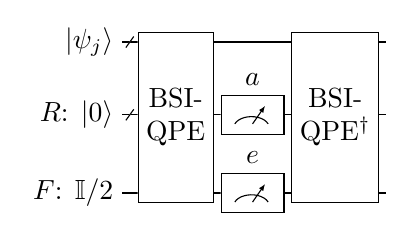
\begin{tikzpicture}
\begin{yquant*}
% init {$\eta$ ancillas} (a);
qubit {$\ket{\psi_j}$} system;
qubit {$R$: $\ket{0}$} a;
qubit {$F$: $\mathbb{I}/2$} f;

slash system;
slash a;
hspace {0.1cm} -;

box {BSI-\\QPE} (a,system,f);

["$a$",type=qubit]
measure a;

["$e$",type=qubit]
measure f;

box {BSI-\\QPE$^{\dagger}$} (a,system,f);
\end{yquant*}
\end{tikzpicture}

\caption{Quantum circuit for implementing projective measurement $E_{ae}$.}
\label{fig:Ecircuit}
\end{figure}
This measurement gives us $(-1)^ea$, which approximates the energy of the initial state. Because $E_{ae}$ is implemented as a projective measurement, its inverse BSI-QPE does not in general disentangle the work register. 
% The post-measurement registers $R, F$ are retained and reused in all subsequent $P_s^{ae}$ and $Q_s^{ae}$ measurements in the same update.
\subsection{Update}
\label{section:update}
After measuring the initial energy we must apply an update to our state. In quantum metropolis this update comes in the form of a unitary operator $C$ chosen from some set $\mathcal{C}$ according to some probability measure $d\mu(C)$. It is essential for the purposes of detailed balance that the probability of choosing $C \in \mathcal{C}$ is equal to the probability of choosing $C^{\dagger} \in \mathcal{C}$ (which is alternatively expressed as $d\mu(C) = d\mu(C^{\dagger})$).
\subsection{Accept or Reject}
\label{section:acceptprob}
After applying our unitary update $C$ we must decide whether to accept or reject this update. To ensure the probability of acceptance is approximately $\tilde{f}_{E_aE_b}$, we use a combination of phase estimation, controlled rotations and single-qubit measurement (illustrated in Fig.~\ref{fig:Qcircuit}). First we apply phase estimation to the same registers $R, F$ used by $E_{ae}$. On the joint BSI-QPE space this operation is
\begin{equation}
  \sum_{j,b,p}G_j^{bp}\otimes\ket{b}\bra{p}\otimes\ket{\psi_j}\bra{\psi_j}
\end{equation}
Then, using the known initial energy estimate results $a$ and $e$, we perform a $W_{abde}$ rotation on $M$, which was initialized to $\ket{0}$ at the beginning of the update, controlled by $b$ from $R$ and $d$ from $F$:
\begin{equation}
    W_{abde} = \begin{pmatrix}
        \sqrt{1 - f_{abde}} & \sqrt{f_{abde}}\\
       \sqrt{f_{abde}} & -\sqrt{1 - f_{abde}}
    \end{pmatrix}
\end{equation}
Therefore, upon measuring this ancilla qubit the probability of measuring $s=1$ is given by $f_{abde}$, which we choose to approximate $\tilde f_{E_aE_b}$. This alone is insufficient to prove that quantum Metropolis converges to a Gibbs state, but it highlights the similarity with classical Metropolis. In Section~\ref{section:why} we analyse convergence rigorously.

If we measure $s=0$ (reject), then we proceed by applying $W_{abde}^{\dagger}$ ($=W_{abde}$) again after the measurement before applying inverse phase estimation and $C^{\dagger}$, to make the whole sequence ($Q_s^{ae}$) a projective binary measurement:
\begin{multline} 
    Q_s^{ae} = \sum_{j,p,q,b,d}  C^{\dagger}\ket{\psi_j}\bra{\psi_j}C \otimes \ket{q}\bra{p} \otimes\\ G_j^{bq\dagger}\ket{d}\bra{d}G_j^{bp}\otimes R^{abde}_s
\end{multline}
where $R^{abde}_s = W_{abde}\ket{s}\bra{s}W_{abde}$. If instead we measure $s=1$ (accept) we simply measure the energy register and then apply inverse BSI-QPE. We represent this accept process as $L^{ade}_b$ as defined in Fig.~\ref{fig:LQ_circuit} and gives the following operator:
\begin{multline}
    L^{ade}_b =\sum_{j,p,q}\ket{\psi_j}\bra{\psi_j}C \otimes \ket{q}\bra{p} \otimes\\ G^{bq\dagger}_j \ket{d}\bra{d}G^{bp}_j \otimes \ket{1}\bra{1}W_{abde}
\end{multline}

The $R,F$ registers in the first $Q_s^{ae}$ measurement are the same registers used in $E_{ae}$, not separately initialized registers. Every later $P_s^{ae}$ and $Q_s^{ae}$ measurement in the update reuses these registers without resetting them. The acceptance-rotation qubit $M$ is initialized to $\ket{0}$ once and is similarly reused in every $Q_s^{ae}$. This common-register structure is shown in Fig.~\ref{fig:fullcircuit} and is required for the Marriott--Watrous rewinding argument below.
\begin{figure}
\begin{tikzpicture}
\begin{yquant*}
% init {$\eta$ ancillas} (a);
qubit {$\ket{\psi_j}$} system;
qubit {$R, F$} a;
qubit {$M:\ket{0}$} f;

slash system;
slash a;
hspace {0.1cm} -;
box {$C$} (system);
box {BSI-\\QPE} (a,system);
[multictrl]
box {$W_{abde}$} (f) ~ a;



["$s$",type=qubit]
measure f;
% text {$\ket{b}$} (a);


[multictrl]
box {$W_{abde}$} (f) ~ a;

box {BSI-\\QPE$^{\dagger}$} (a,system);
box {$C^{\dagger}$} (system);
\end{yquant*}
\end{tikzpicture}

\caption{Quantum circuit for implementing projective measurement $Q_s^{ae}$. The BSI-QPE registers $R, F$ are the same registers used by $E_{ae}$ and $P_s^{ae}$, while the rotation qubit $M$ is reused in every $Q_s^{ae}$ without being reset. It is necessary to apply $W_{abde}$ before and after the measurement to make the whole measurement projective (as $W_{abde}^{\dagger}=W_{abde}$). The slashed control denotes multiplexed control \cite{low2024trading}.}
\label{fig:Qcircuit}
\end{figure}

\begin{figure}
\begin{tikzpicture}
\begin{yquant*}
% init {$\eta$ ancillas} (a);
qubit {$\ket{\psi_j}$} system;
qubit {$R,F$} a;
qubit {$M$} f;

slash system;
slash a;
hspace {0.1cm} -;
box {$C$} (system);
box {BSI-\\QPE} (a,system);
[multictrl]
box {$W_{abde}$} (f) ~ a;



["$s=1$",type=qubit]
measure f;
["$b\>\>d$",type=qubit]
measure a;
% text {$\ket{b}\bra{b}$} (a);
box {BSI-\\QPE$^{\dagger}$} (a,system);
\end{yquant*}
\end{tikzpicture}

\caption{Quantum circuit for implementing accept process $L_b^{ade}$.}
\label{fig:LQ_circuit}
\end{figure}
\subsection{Rejection process}
Upon rejection in the classical algorithm we can simply revert back to an earlier copy we made of the initial state or we may be able to reverse the update applied. However, in the quantum setting the no-cloning principle rules out the former and the irreversibility of measurement rules out the latter. Therefore, we need a new technique to return to our initial state.

We use an iterative sequence of binary projective measurements similar to the QMA verification amplification of Marriott and Watrous \cite{MarriottWatrous}. The first measurement $Q_s^{ae}$ has already been introduced, whilst the second $P_s^{ae}$ simply reports whether the state has returned to the initial energy:


\begin{equation}
    P^{ae}_1 = \sum_{j,p,q} \left( \ket{\psi_j}\bra{\psi_j} \otimes \ket{q}\bra{p} \otimes G_j^{aq\dagger}\ket{e}\bra{e}G_j^{ap} \right)
\end{equation}
\begin{multline}
    P^{ae}_0 = \sum_{j,p,q} \sum_{b}\bigg( \ket{\psi_j}\bra{\psi_j} \otimes \ket{q}\bra{p} \otimes \\G_j^{bq\dagger}(\mathbb{I} - \delta_{ab}\ket{e}\bra{e})G_j^{bp}  \bigg)
\end{multline}
This measurement is conducted as demonstrated by Fig.~\ref{fig:Pcircuit}. The register on which $P_s^{ae}$ acts is the same persistent register $R$ used by $E_{ae}$ and $Q_s^{ae}$, as shown in Fig.~\ref{fig:fullcircuit}; $P_s^{ae}$ acts trivially on the rotation qubit $M$.
\begin{figure}
\begin{tikzpicture}
\begin{yquant*}
% init {$\eta$ ancillas} (a);
qubit {$\ket{\psi_j}$} system;
qubit {$R,F$} a;
qubit {$\ket{0}$} f;

slash system;
slash a;
hspace {0.1cm} -;
box {BSI-QPE} (a,system);

[multictrl]
box { $X$} f ~ a;

["$s$",type=qubit]
measure f;


box {BSI-QPE$^{\dagger}$} (a,system);
\end{yquant*}
\end{tikzpicture}

\caption{Quantum circuit for implementing projective measurement $P_s^{ae}$. The displayed target qubit is only a pointer used to record the binary outcome and need not persist between measurements. The controlled $X$ gate is triggered only by the state $\ket{a}\ket{e}$ of the persistent register $R$.}
\label{fig:Pcircuit}
\end{figure}
\begin{figure}
    \centering
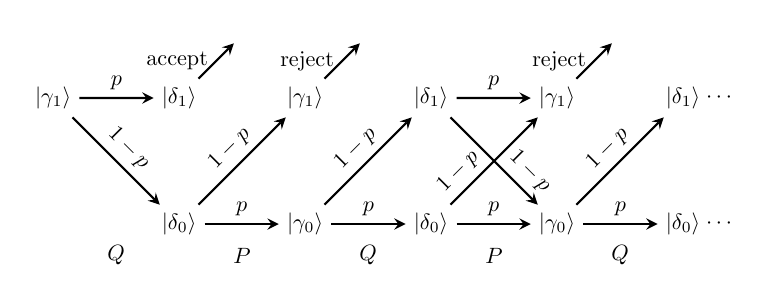
\begin{tikzpicture}[node distance=2cm, >=stealth, thick, scale=0.8, transform shape]
    \node (g-1t) at (0,2) {$|\gamma_1\rangle$};
    \node (s0t)  at (2,2) {$|\delta_1\rangle$};
    \node (s0)  at (2,0) {$|\delta_0\rangle$};
    \node (g0)  at (4,0) {$|\gamma_0\rangle$};
    \node (s1)  at (6,0) {$|\delta_0\rangle$};
    \node (g1)  at (8,0) {$|\gamma_0\rangle$};
    \node (s2)  at (10,0) {$|\delta_0\rangle$};
    \node (...1) at (10.6,0) {$\cdots$};
    \node (...2) at (10.6,2) {$\cdots$};
    
    \node (a) at (3,3) {};
    \node (r1) at (5,3) {};
    \node (r2) at (9,3) {};
    
    \node (g1t) at (4,2) {$|\gamma_1\rangle$};
    \node (s1t) at (6,2) {$|\delta_1\rangle$};
    \node (g2t) at (8,2) {$|\gamma_1\rangle$};
    \node (s2t) at (10,2) {$|\delta_1\rangle$};
    
    % Transitions
    \draw[->] (s0) -- node[above] {$p$} (g0);
    \draw[->] (g0) -- node[above] {$p$} (s1);
    \draw[->] (s1) -- node[above] {$p$} (g1);
    \draw[->] (g1) -- node[above] {$p$} (s2);
    
    \draw[->] (s0) -- node[above,sloped] {$1-p$} (g1t);
    \draw[->] (g0) -- node[above ,sloped] {$1-p$} (s1t);
    \draw[->] (s1) -- node[above left,sloped] {$1-p$} (g2t);
    \draw[->] (s1t) -- node[above] {$p$} (g2t);
    \draw[->] (g-1t) -- node[above] {$p$} (s0t);
    
    \draw[->] (s1t) -- node[above right,sloped] {$1-p$} (g1);
    \draw[->] (g1) -- node[above ,sloped] {$1-p$} (s2t);
    \draw[->] (g-1t) -- node[above ,sloped] {$1-p$} (s0);

    \draw[->] (s0t) -- node[left] {accept} (a);
    \draw[->] (g1t) -- node[left] {reject} (r1);
    \draw[->] (g2t) -- node[left] {reject} (r2);

    % Labels
    \node at (1,-0.5) {$Q$};
    \node at (3,-0.5) {$P$};
    \node at (5,-0.5) {$Q$};
    \node at (7,-0.5) {$P$};
    \node at (9,-0.5) {$Q$};
\end{tikzpicture}
    \caption{Markov chain showing the transition probability between the 4 states of a single invariant subspace $\lambda$ (with $p = p^{ae\lambda}$) upon each projective measurement. The full rejection process is a mixture of such chains weighted by $|c^{aej}_{\lambda}|^2$.}
    \label{fig:transitions}
\end{figure}
\begin{figure*}
    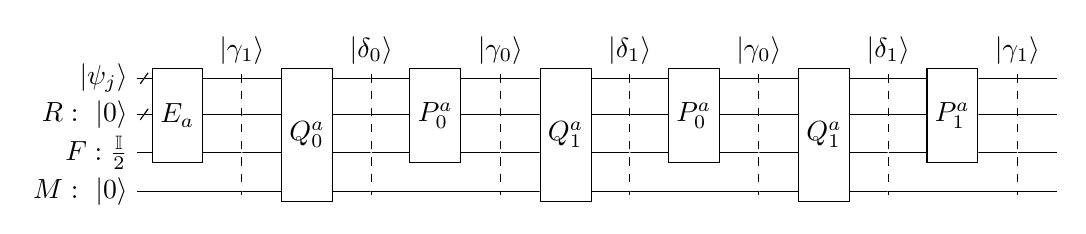
\begin{tikzpicture}
\begin{yquant*}
qubit {$\ket{\psi_j}$}  s;
qubit {$R:\ \ket{0}$} anc;
qubit {$F: \frac{\mathbb{I}}{2}$} f;
qubit {$M:\ \ket{0}$} m;
slash s;
slash anc;
hspace {0.1cm} -;
box {$E_a$} (s,anc,f);
["$\ket{\gamma_1}$"]
barrier (-);
box {$Q^a_0$} (s,anc,f, m);
["$\ket{\delta_0}$"]
barrier (-);
box {$P^a_0$} (s,anc,f);
["$\ket{\gamma_0}$"]
barrier (-);
box {$Q^a_1$} (s,anc,f, m);
["$\ket{\delta_1}$"]
barrier (-);
box {$P^a_0$} (s,anc,f);
["$\ket{\gamma_0}$"]
barrier (-);
box {$Q^a_1$} (s,anc,f, m);
["$\ket{\delta_1}$"]
barrier (-);
box {$P^a_1$} (s,anc,f);
["$\ket{\gamma_1}$"]
barrier (-);
\end{yquant*}
\end{tikzpicture}
\caption{A successfully completed rejection procedure. The same BSI-QPE registers $R, F$ is reused by $E_{ae}$ and every $P_s^{ae}$ and $Q_s^{ae}$; the qubit $M$ is reused by every $Q_s^{ae}$. This circuit corresponds to a term in $\mathcal{B}(2)[\rho]$ for $\{s_n\}=\{1,1\}$ and, within a single invariant subspace $\lambda$ (see Section~\ref{section:rejection}), occurs with probability $(1-p^{aej}_{\lambda})^4(p^{aej}_{\lambda})^2$. The state labels at the barriers denote the corresponding states of each invariant subspace.}
\label{fig:fullcircuit}
\end{figure*}

The iterative process proceeds as follows after measuring $s=0$ (reject) from the initial $Q_s^{ae}$ measurement: 
\begin{enumerate}
    \item Measure $P_s^{ae}$
        \begin{enumerate}
            \item If $s=1$ \textbf{terminate} as the state has returned to the approximate energy of the initial state.
            \item If $s=0$ continue.
        \end{enumerate}
    \item Measure $Q_s^{ae}$
    \item Repeat up to a maximum of $n^*$ iterations
\end{enumerate}
The two measurements $P^{ae}_s$ and $Q^{ae}_s$ do not scatter the state over the whole Hilbert space. They confine it to a family of mutually orthogonal \emph{two-dimensional} subspaces, and within any one of them the state simply ping-pongs between two pairs of vectors, $\ket{\gamma_0},\ket{\gamma_1}$ and $\ket{\delta_0},\ket{\delta_1}$, according to the four-state Markov chain of Fig.~\ref{fig:transitions}. Reaching $\ket{\gamma_1}$ means the rewind has succeeded and the state has returned to its original energy. Because the chain is this simple, the probability that $n^*$ attempts all fail can be read off directly, which is what Eq.~\eqref{eq:probabilty_of_rejection} does. 

To see this let us consider the action of the rejection process on each eigenvector $\ket{\psi_j}$ of $H$. To handle the mixed initial state of $F$, purify $\frac{\mathbb{I}}{2}$ as $\ket{\Phi}_{FF'}=\frac{1}{\sqrt{2}}\sum_f\ket{f}_F\ket{f}_{F'}$, where the reference $F'$ is never acted upon. Conditioned on the outcome $(a,e)$, the corresponding pure post-measurement state is
\begin{equation}
    \frac{(E_{ae}\otimes\mathbb I_{F'})\ket{\psi_j}\ket{0}_R\ket{\Phi}_{FF'}\ket{0}_M}
    {\|(E_{ae}\otimes\mathbb I_{F'})\ket{\psi_j}\ket{0}_R\ket{\Phi}_{FF'}\ket{0}_M\|}
    = \sum_{\lambda} c_{\lambda}^{aej}\ket{\gamma_1^{ae \lambda}}.
\end{equation}
Tracing out $F'$ recovers the physical evolution from $\frac{\mathbb{I}}{2}$. Because $P_1^{ae}E_{ae}=E_{ae}$, this state is a $+1$ eigenstate of $P_1^{ae}$ (with all projectors implicitly extended by $\mathbb I_{F'}$). Furthermore, $P_1^{ae}$ commutes with $P^{ae}_1Q^{ae}_0P^{ae}_1$, so the two operators are jointly diagonalizable and the expansion above may be taken in their joint eigenstates. The untouched reference is absorbed into the degeneracy label $\lambda$.
Writing the eigenvalue of $\ket{\gamma^{ae\lambda}_1}$ as $1-p^{ae\lambda}$, we have: \begin{align}1-p^{ae\lambda}&=\bra{\gamma^{ae\lambda}_1}P^{ae}_1Q^{ae}_0P^{ae}_1\ket{\gamma^{ae\lambda}_1} \\&=\|Q^{ae}_0P^{ae}_1\ket{\gamma^{ae\lambda}_1}\|^2\\ &= 1-\|Q^{ae}_1\ket{\gamma^{ae\lambda}_1}\|^2
\end{align}
so $p^{ae\lambda} = \|Q^{ae}_1\ket{\gamma^{ae\lambda}_1}\|^2$, and the probability of accepting the update is given by the mixture $p_{aej} = \sum_{\lambda}|c^{aej}_{\lambda}|^2p^{ae\lambda}$. Therefore, for each $\lambda$ with $p^{ae\lambda} \in (0,1)$ we can define the following 2D invariant subspace (we have suppressed the $ae\lambda$ labels for the remainder of this section for clarity, writing $\ket{\gamma_1} = \ket{\gamma^{ae\lambda}_1}$ and $p = p^{ae\lambda}$):
\begin{align}
    \ket{\delta_0} &= \frac{Q^{ae}_0P^{ae}_1\ket{\gamma_1}}{\sqrt{1-p}} &\ket{\delta_1} &= \frac{Q^{ae}_1P^{ae}_1\ket{\gamma_1}}{\sqrt{p}} \\
    \ket{\gamma_0} &= \frac{P^{ae}_0Q^{ae}_0\ket{\delta_0}}{\sqrt{p}} &\ket{\gamma_1} &= \frac{P^{ae}_1Q^{ae}_0\ket{\delta_0}}{\sqrt{1-p}}
\end{align}
From these definitions the following relations can be deduced:
\begin{align}
\begin{split}
\label{eq:deltagamma0}
    P^{ae}_1 \ket{\gamma_1} &= (Q^{ae}_0+Q^{ae}_1)P^{ae}_1 \ket{\gamma_1}\\
    &= Q^{ae}_0P^{ae}_1 \ket{\gamma_1}+Q^{ae}_1P^{ae}_1 \ket{\gamma_1}\\
    &= \sqrt{1-p} \ket{\delta_0} + \sqrt{p}\ket{\delta_1}\\
    Q^{ae}_0\ket{\delta_0} &= \sqrt{p} \ket{\gamma_0} + \sqrt{1-p} \ket{\gamma_1}
\end{split}
\end{align}
As $P^{ae}_1 \ket{\gamma_1} = \ket{\gamma_1}$ and $Q^{ae}_0\ket{\delta_0} = \ket{\delta_0}$ we can simplify the above and then through substitution deduce the remaining relations:
\begin{align}
\begin{split}
\label{eq:deltagamma1}
        \ket{\delta_1} &= -\sqrt{1-p} \ket{\gamma_0} + \sqrt{p} \ket{\gamma_1}\\
    \ket{\gamma_0} &= \sqrt{p} \ket{\delta_0} - \sqrt{1-p}\ket{\delta_1}
\end{split}
\end{align}
Therefore it is clear that each measurement transitions the state from one of $\ket{\delta_i}$ to one of $\ket{\gamma_i}$ or vice versa, whilst remaining within the same 2D invariant subspace. As the subspaces corresponding to different $\lambda$ are mutually orthogonal (which follows from the orthogonality of the $\ket{\gamma^{ae\lambda}_1}$ together with the relations above) and each is preserved by both measurements, the subspaces do not mix at any point during the rejection process. The probability of these transitions are trivially deduced from \eqref{eq:deltagamma0} and \eqref{eq:deltagamma1}, and can be seen in Fig.~\ref{fig:transitions}.


From this we can calculate the probability of attempting to reject and then failing the rejection process within a single invariant subspace to be $p(1-p)(p^2 +(1-p)^2)^{n^*}$. As the subspaces do not mix, the overall failure probability $p_a^{fail}$ is the corresponding mixture over subspaces (reinstating the suppressed labels):
\begin{equation}
   p_{aej}^{fail} =  \sum_{\lambda}|c^{aej}_{\lambda}|^2p^{ae\lambda}(1-p^{ae\lambda})((p^{ae\lambda})^2 +(1-p^{ae\lambda})^2)^{n^*}
\end{equation}
For all $p \in [0,1]$ we have: 
\begin{equation}
    p(1-p)(p^2 +(1-p)^2)^{n^*} \leq \frac{1}{2(n^*+1)} \left(\frac{n^*}{n^*+1}\right)^{n^*}
\end{equation}
Therefore, as $\sum_{\lambda}|c^{aej}_{\lambda}|^2=1$ we have:
\begin{equation}
    \label{eq:probabilty_of_rejection}
   p_{aej}^{fail} \leq \frac{1}{2(n^*+1)} \left(\frac{n^*}{n^*+1}\right)^{n^*} \leq \frac{1}{2n^*}
\end{equation}
If the rejection process fails then the whole algorithm fails irrecoverably and must be reset to the original initial state.

We have chosen to present the rewinding mechanism through this lens of projective measurements and invariant subspaces in an attempt to make the procedure more intuitive. We refer the reader to the treatment via Jordan's Lemma in the original Quantum Metropolis paper \cite{Temme_2011} for an alternative approach to reach the same conclusions.
\label{section:rejection}

\section{Why it works}
\label{section:why}
The classical Metropolis-Hastings algorithm works by constructing a Markov Chain through proposing and accepting/rejecting moves with probabilities determined by the energy difference between the initial and modified states. The transition matrix of this Markov chain is in detailed balance with respect to the Gibbs state, implying that the Gibbs state is a fixed point of the Markov chain. As Markov chain is also ergodic, it is known that it must have a single unique fixed point and converge towards it. Therefore, the Markov chain converges to the Gibbs state.

In the quantum Metropolis algorithm we similarly construct a quantum Markov chain by proposing and accepting or rejecting moves based on energy differences. Because the energy differences cannot be resolved exactly, we cannot prove exact detailed balance and instead use a notion of approximate quantum detailed balance (Definition~\ref{def:approxdb}) that incorporates additive errors from the nonzero, exponentially suppressed tails of BSI-QPE. We use this theorem to establish that the Gibbs state is approximately invariant. Further choosing the update set $\{C\}$ to be universal ensures ergodicity and hence the uniqueness of the fixed point \cite{Temme_2011}. The closeness of the actual fixed point to this approximately invariant point additionally depends on the mixing properties of the channel. We formalise these statements into the following main result of the paper. Informally, it says: \emph{one round of the algorithm moves the Gibbs state only a little, and the two ways it can move are both controllable --- by adding ancilla qubits, and by allowing more rewinding attempts.} Formally:

\begin{theorem}
\label{theorem:main}
Let $\mathcal{E}$ be one update round of the quantum Metropolis algorithm of Section~\ref{section:algorithm}, implemented with $\eta$ ancillas, evolution time $t = \frac{1}{16\|H\|}$, rewinding cap $n^*$, an update measure satisfying $d\mu(C)=d\mu(C^{\dagger})$, and window functions satisfying the conditions of Appendix~\ref{section:appendix} with truncation bandwidth $\mu = \Omega(\frac{1}{\nu}\log n^*)$, $\mu < \min(\frac{N}{96\pi}, \frac{\frac{N}{8}}{4n^*+6}, \frac{Nt}{384\pi\beta(4n^*+6)})$. Then
\begin{equation}
   \|\mathcal{E}[\sigma_G] - \sigma_G\|_* = O\left(\max\left( n^{*\frac{7}{2}}\sqrt{\frac{\beta\|H\| }{2^{\eta}}}\mu^{\frac{3}{2}},\frac{1}{n^*}\right)\right).
\label{eq:theoremmain}
\end{equation}
If, in addition, $\mathcal{E}^{\ell}$ is strictly trace-norm contracting with factor $k<1$ for some integer $\ell\geq1$, then $\mathcal{E}$ has a unique fixed point $\sigma^*$, is approached exponentially fast, and $\|\sigma^*-\sigma_G\|_* \leq \frac{\ell}{1-k}\|\mathcal{E}[\sigma_G] - \sigma_G\|_*$ (Theorem~\ref{theorem:error_bound}). If moreover $\frac{\ell}{1-k}\leq\tau_0$ with $\tau_0$ independent of $\eta$, $n^*$ and the window parameters, then $\sigma_G$ is prepared to any trace-norm accuracy at polynomial cost (Corollary~\ref{corollary:polycost}).
\end{theorem}

The two terms in Eq.~\eqref{eq:theoremmain} have quite different origins, and it is worth separating them before the proof. The first, $n^{*\frac{7}{2}}\sqrt{\beta\|H\|2^{-\eta}}\mu^{\frac{3}{2}}$, is the residual \emph{bias} left by an imperfect energy estimate: the acceptance probability is computed from a readout that is only accurate to within the bandwidth $\mu$, so detailed balance holds only up to a multiplicative error, and every extra rewinding attempt gives that error another chance to act. It shrinks exponentially in the number of ancilla qubits $\eta$. The second, $1/n^*$, is the probability that the rewind never terminates and the whole run must be discarded (Eq.~\eqref{eq:probabilty_of_rejection}); it shrinks as the cap $n^*$ is raised.

The proof of this theorem occupies the remainder of this section and is broken down into a number of steps. First, in Section~\ref{section:detailedbalancedef} we define our approximate detailed balance criteria which allow us to consider each branch of the original $\mathcal{E}$ CP-map separately. We then proceed in Section~\ref{section:proofbranchwisebalance} to prove the acceptance and rejection branches of our update step satisfy our branch-wise approximate detailed balance criteria. Finally, in Section~\ref{sec:combine} use Lemma~\ref{theorem:quantumapproximatedeatildedbalance} to combine these error terms to demonstrate that the Gibbs state is approximately stationary. We go further and show that by taking certain assumptions we can show the Gibbs state is close to the fixed point of the map, and that the map converges exponentially quickly towards this fixed point.
\subsection{Approximate Quantum Detailed Balance}
\label{section:detailedbalancedef}
In the classical setting, detailed balance can be verified by comparing each transition with its reverse, weighted by the Gibbs probabilities. Our attempts to replicate this methodology in the quantum setting are frustrated by two obstacles. First, due to inexact quantum phase estimation, we cannot exactly resolve the energies of our states and hence cannot implement the exact transition amplitudes that would lead to quantum detailed balance. Second, some branches of the weighted adjoint map agree closely not with the corresponding branch of the original map, but with a differently labelled one. In this section we therefore present a formulation of approximate quantum detailed balance that is verified branch by branch, allows branches to be paired with differently labelled partners, and accommodates the additive errors introduced by the truncation step.

For any completely positive map $\mathcal{M}$ with Kraus decomposition $\mathcal{M}[\rho] = \sum_{j} A_{j}\rho A^{\dagger}_{j}$ and any density matrix $\sigma$, we define
\begin{align}
    \mathcal{M}_{\sigma}[\rho] &= \sum_{j} A_{j}\sigma^{\frac{1}{2}}\rho\,\sigma^{\frac{1}{2}} A^{\dagger}_{j} = \mathcal{M}\big[\sigma^{\frac{1}{2}}\rho\,\sigma^{\frac{1}{2}}\big],\\
    \mathcal{M}^{\dagger}[\rho] &= \sum_j A^{\dagger}_j \rho A_j,\\
    \mathcal{M}^*_{\sigma}[\rho] &= \sum_{j} \sigma^{\frac{1}{2}}A^{\dagger}_{j}\rho A_{j}\sigma^{\frac{1}{2}} = \sigma^{\frac{1}{2}}\mathcal{M}^{\dagger}[\rho]\,\sigma^{\frac{1}{2}}.
\end{align}

\begin{definition}[Approximate quantum detailed balance]
\label{def:approxdb}
A completely positive map $\mathcal{M}$ satisfies $\epsilon$-approximate quantum
detailed balance with respect to $\sigma$ if, for every operator $X$,
\begin{equation}
    \|\mathcal{M}^*_{\sigma}[X] - \mathcal{M}_{\sigma}[X]\|_* \leq \epsilon\|X\|.
\end{equation}
\end{definition}

Our strategy is to establish the $X=\mathbb{I}$ instance of Definition~\ref{def:approxdb}, which is all Lemma~\ref{theorem:quantumapproximatedeatildedbalance} requires, for each acceptance and rejection branch of $\mathcal{E}$ separately. Lemma~\ref{lemma:1} compares components paired by a relabelling $c\mapsto c'$. For each input basis state, its hypothesis requires the corresponding weighted outputs to differ only by a small diagonal rescaling; its conclusion converts these multiplicative discrepancies $\epsilon_{m}$ into a trace-norm bound. The lemma is stated for two maps $\mathcal{M}$ and $\mathcal{M}'$ because, in the rejection step, we can establish this criterion only after slightly modifying the acceptance rotations in the weighted adjoint map. We bound the error introduced by this modification separately.

\begin{lemma}[Branch-wise Approximate Detailed Balance Criterion]
\label{lemma:1}
Let $\mathcal{M}$ and $\mathcal{M'}$ be completely positive maps on $d$-dimensional density matrices admitting the same decomposition $\mathcal{M} = \sum_{c\in\mathcal{X}} \mathcal{M}_c$, $\mathcal{M'} = \sum_{c\in\mathcal{X}} \mathcal{M'}_c$ into completely positive maps $\mathcal{M}_c$ and $\mathcal{M}'_c$, and let $\sigma = \sum_j \sigma_j \ket{\psi_j}\bra{\psi_j}$ be a density matrix diagonal in the orthonormal basis $\{\ket{\psi_j}\}$. Suppose there exists a bijection $c \mapsto c'$ of $\mathcal{X}$ such that, for every $j,k,c,l,m$,
\begin{multline}
    \bra{\psi_m}\mathcal{M}'^*_{c'\sigma}[\ket{\psi_j}\bra{\psi_k}]\ket{\psi_l}
    =\\(1+u^{c}_{jm})(1+ u^{c}_{kl})
    \bra{\psi_m}\mathcal{M}_{c\sigma}[\ket{\psi_j}\bra{\psi_k}]\ket{\psi_l}
    \label{eq:approximate_quantum_detailed_balance_condition}
\end{multline}
where the $u^{c}_{jl}$ are real and satisfy $|u^{c}_{jl}| \leq \epsilon_m$. Then, for every operator $X$,
 \begin{equation}
    \|\mathcal{M}'^*_{\sigma}[X]-\mathcal{M}_{\sigma}[X] \|_* \leq (2\epsilon_m+\epsilon_m^2)\|\mathcal{M}[\sigma]\|_*\|X\| \label{eq:lemma2output}
\end{equation}
where $\|\cdot\|_*$ is trace-norm.
\end{lemma}

\begin{proof}
 By definition $\mathcal{M}[\sigma]=\mathcal{M}_{\sigma}[\mathbb{I}]$. By linearity and the bijectivity of $c \mapsto c'$:
    \begin{equation}
        \mathcal{M}'^*_{\sigma}[X] = \sum_{c}\mathcal{M}'^*_{c\sigma}[X] = \sum_{c}\mathcal{M}'^*_{c'\sigma}[X]
    \end{equation}
    Define $M^{jc} = \mathcal{M}_{c\sigma}[\ket{\psi_j}\bra{\psi_j}]$ and $D^{jc}=\sum_l(1+u_{jl}^{c})\ket{\psi_l}\bra{\psi_l}$, let $\mathcal{M}_{c\sigma}[\rho]=\sum_i K^c_i\rho K^{c\dagger}_i$ be a Kraus decomposition, and let $\tilde K^c_i=\sum_j D^{jc}K^c_i\ket{\psi_j}\bra{\psi_j}$. Equation~\eqref{eq:approximate_quantum_detailed_balance_condition} is then, by linearity, the operator identity
    \begin{equation}
        \mathcal{M}'^*_{c'\sigma}[X]=\sum_i\tilde K^c_iX\tilde K^{c\dagger}_i
    \end{equation}
    Moreover, $\mathcal{M}_{\sigma}[X] = \sum_{i,c}K^c_iXK^{c\dagger}_i$, so we have:
    \begin{multline}
        \|\mathcal{M}'^*_{\sigma}[X]-\mathcal{M}_\sigma[X]\|_* \leq \\\sum_{i,c}\Big\|\left(\tilde K^c_iX\tilde K^{c\dagger}_i-K^c_iXK^{c\dagger}_i\right)\Big\|_*
    \end{multline}
    Writing $W^c_i=\tilde K^c_i-K^c_i$, we have:
    \begin{multline}
        \tilde K^c_iX\tilde K^{c\dagger}_i-K^c_iXK^{c\dagger}_i = W^c_iXK^{c\dagger}_i + K^c_iXW^{c\dagger}_i \\+ W^c_iXW^{c\dagger}_i
    \end{multline}
    By the generalised H\"older's inequality for Schatten norms we have:
    \begin{equation}
        \Big\|W^c_iXK^{c\dagger}_i\Big\|_* \leq \|W^c_i\|_2\|X\| \|K^{c\dagger}_i\|_2
    \end{equation}
    Further by Cauchy-Schwarz:
    \begin{equation}
        \sum_i\Big\|W^c_iXK^{c\dagger}_i\Big\|_* \leq \|X\| \sqrt{\sum_i \|W^c_i \|^2_2}\sqrt{\sum_i \|K_i^{c\dagger}\|^2_2}
    \end{equation}
    and similarly for the remaining terms. We have 
    
    \begin{align}
        \sum_i \|K^{c\dagger}_i\|^2_2&=\sum_i\operatorname{Tr}[K^{c\dagger}_iK^{c}_i]=\operatorname{Tr}[\mathcal{M}_{c\sigma}[\mathbb{I}]]\\
        &=\sum_j \operatorname{Tr}[M^{jc}]
    \end{align} and similarly $\sum_i \|W^c_i\|^2_2=\sum_j \operatorname{Tr}[V^{jc}M^{jc}V^{jc}]$ where $V^{jc} = D^{jc}-\mathbb{I}$, which satisfies $\|V^{jc}\|\leq\epsilon_m$. Further, as $M^{jc}$ is positive semi-definite:
    \begin{equation}
       \operatorname{Tr}[V^{jc}M^{jc}V^{jc}] \leq \|V^{jc}\|^2\, \operatorname{Tr}[M^{jc}] \leq \epsilon_m^2\, \operatorname{Tr}[M^{jc}]
    \end{equation}
    Therefore,
    \begin{equation}
        \|\mathcal{M}'^*_{\sigma}[X]-\mathcal{M}_\sigma[X]\|_* 
        \leq (2\epsilon_m+\epsilon_m^2)\|X\|\sum_{j,c}\operatorname{Tr}[M^{jc}] 
    \end{equation}
    Finally:
    \begin{equation}
        \sum_{j,c}\operatorname{Tr}[M^{jc}] = \operatorname{Tr}[\mathcal{M}_{\sigma}[\mathbb{I}]] = \operatorname{Tr}[\mathcal{M}[\sigma]] = \|\mathcal{M}[\sigma]\|_*
    \end{equation}
\end{proof}

We use Lemma~\ref{lemma:1} to show that our band-limited maps satisfy the branch-wise approximate detailed balance
criterion for the acceptance branch $\tilde{\mathcal{A}}$ and every rejection branch $\tilde{B}(n)$. We then add the additive error ($\epsilon_a$) between the original map and the band-limited map to show approximate quantum detailed balance for the acceptance and rejection branches. Finally, we combine these using Lemma~\ref{theorem:quantumapproximatedeatildedbalance} to show the Gibbs state is approximately stationary.
\begin{lemma}[Approximate detailed balance implies approximate stationarity]
\label{theorem:quantumapproximatedeatildedbalance}
Let $\mathcal{E} = \sum_j \mathcal{M}_j$ be a completely positive trace-preserving map on $d$-dimensional density matrices, with each $\mathcal{M}_j$ completely positive, and let $\sigma$ be a density matrix. If each $\mathcal{M}_j$ satisfies $\epsilon^j$-approximate quantum detailed balance with respect to $\sigma$ (Definition~\ref{def:approxdb}), or merely its $X=\mathbb{I}$ instance, then
\begin{equation}
     \|\mathcal{E}[\sigma]-\sigma\|_* \leq \sum_j\min\left(\epsilon^j, 2\|\mathcal{M}_j[\sigma]\|_*\right)
\end{equation}
\end{lemma}
\begin{proof}
    By the triangle inequality we have:
    \begin{equation}
        \|\mathcal{E}^*_{\sigma}[\mathbb{I}]-\mathcal{E}[\sigma]\|_* \leq \sum_j \|\mathcal{M}^*_{j\sigma}[\mathbb{I}]-\mathcal{M}_{j}[\sigma]\|_*
    \end{equation}
    As $\mathcal{E}$ is trace-preserving, we know that:
    \begin{equation}
        \mathcal{E}^*_{\sigma}[\mathbb{I}] = \sum_{j} \sigma^{\frac{1}{2}}A^{\dagger}_{j} A_{j}\sigma^{\frac{1}{2}} = \sigma
    \end{equation}
    Therefore,
    \begin{equation}
        \|\sigma - \mathcal{E}[\sigma]\|_* \leq \sum_j \|\mathcal{M}^*_{j\sigma}[\mathbb{I}]-\mathcal{M}_{j}[\sigma]\|_*
    \end{equation}
    By assumption (with $X=\mathbb{I}$, $\|\mathbb{I}\|=1$) we have
    \begin{equation}
        \|\mathcal{M}^*_{j\sigma}[\mathbb{I}]-\mathcal{M}_{j}[\sigma]\|_* \leq \epsilon^j
    \end{equation}
    Further, as both
$\mathcal{M}_{j,\sigma}^{*}[\mathbb{I}]$ and
$\mathcal{M}_j[\sigma]$ are positive semidefinite:
    \begin{align}
        \|\mathcal{M}^*_{j\sigma}[\mathbb{I}]\|_* &= Tr\left[\sum_l \sigma^{\frac{1}{2}} K_{jl}^{\dagger} \mathbb{I} K_{jl} \sigma^{\frac{1}{2}}\right]\\
        &= Tr\left[\sum_l K_{jl}\sigma K_{jl}^{\dagger}\right]\\
        &= \|\mathcal{M}_{j}[\sigma]\|_*
    \end{align}
    Therefore,
    \begin{equation}
         \|\mathcal{M}^*_{j\sigma}[\mathbb{I}]-\mathcal{M}_{j}[\sigma]\|_* \leq 2\|\mathcal{M}_{j}[\sigma]\|_*
    \end{equation}
    Hence,
    \begin{equation}
        \|\sigma-\mathcal{E}[\sigma]\|_* \leq \sum_j \min \left(\epsilon^j, 2\|\mathcal{M}_{j}[\sigma]\|_*\right)
    \end{equation}
\end{proof}

% \begin{widetext}
\subsection{Proof of Theorem~\ref{theorem:main}}
\label{section:proofmain}
We must first express $\mathcal{E}$ as a completely positive trace preserving map:
\begin{equation}
    \mathcal{E}[\rho] = \mathcal{A}[\rho] + \sum_{n=0}^{n^*} \mathcal{B}(n)[\rho] + \mathcal{C}[\rho]
\end{equation}
where $\mathcal{A}$ corresponds to acceptance, $\mathcal{B}(n)$ to successful rejection after $n$ iterations and $\mathcal{C}$ to failing to reject after $n^*$ iterations. Let $\Omega_{RFM} =\ket{0}\bra{0}_R\otimes \frac{\mathbb{I}_F}{2}\otimes\ket{0}\bra{0}_M$ denote the initial state of the persistent ancillas. All occurrences of $E_{ae}$, $P_s^{ae}$, $Q_s^{ae}$ and $L_b^{ade}$ below act on this common ancillary space, with identities on any register on which a given operator acts trivially. Then
\begin{multline}
    \mathcal{A}[\rho] = \int  Tr_{RFM}\bigg[\sum_{a,b,d,e}L_b^{ade} E_{ae} \\( \rho\otimes \Omega_{RFM}) 
     E_{ae}L^{ade\dagger}_b\bigg]d\mu(C)
\end{multline}
\begin{multline}
    \mathcal{B}(n)[\rho] = \int Tr_{RFM}\bigg[\sum_{a,e,\{s\}}P^{ae}_1Q^{ae}_{s_n}\ldots P^{ae}_0Q^{ae}_{s_1}P^{ae}_0Q^{ae}_0E_{ae}\\ ( \rho\otimes \Omega_{RFM})E_{ae}Q^{ae}_0P^{ae}_0Q^{ae}_{s_1}P^{ae}_0\ldots Q^{ae}_{s_n}P^{ae}_1\bigg]d\mu(C)
\end{multline}
\begin{multline}
    \mathcal{C}[\rho] = \rho_0 \int Tr\bigg[\sum_{a,e,\{s\}}P^{ae}_0Q^{ae}_{s_{n^*}}\ldots P^{ae}_0Q^{ae}_{s_1}P^{ae}_0Q^{ae}_0E_{ae}\\ ( \rho\otimes \Omega_{RFM})\\E_{ae}Q^{ae}_0P^{ae}_0Q^{ae}_{s_1}P^{ae}_0\ldots Q^{ae}_{s_{n^*}}P^{ae}_0\bigg]d\mu(C) 
\end{multline}
where $\rho_0$ is the initial state the overall Metropolis algorithm was started from. 
\subsubsection{Approximate quantum detailed balance of $\mathcal{A}$ and $\mathcal{B}$}
\label{section:proofbranchwisebalance}
We demonstrate that $\mathcal{A}$ and $\mathcal{B}$ are in approximate detailed balance by proving \eqref{eq:approximate_quantum_detailed_balance_condition} holds for each of them. We achieve this via the same 4 step proof applied to each map. Here we give a high-level overview of the proof steps, with the proofs themselves laid out in Appendices~\ref{appendix:Aproof} and \ref{appendix:Bproof}:
\begin{enumerate}
    \item \textbf{Truncate.} We replace $\hat \alpha$, $\hat \beta$ by their band-limited versions $\tilde \alpha$, $\tilde \beta$ as in Lemma~\ref{lemma:0}. Then, we use Lemma~\ref{lemma:3} to bound the diamond-norm difference between the original $E^{ae}$, $P_s^{ae}$, $Q_s^{ae}$ measurements and their band-limited replacements. Using Lemma~\ref{lemma:composition} we combine these bounds on the error of each measurement into a diamond-norm bound on the difference between the band-limited map ($\tilde{\mathcal{A}}$, $\tilde{\mathcal{B}}$) and the original ($\mathcal{A}$, $\mathcal{B}$):
        \begin{equation}
    \begin{aligned}
    \|\mathcal{A}_{\sigma_G}[\mathbb{I}] - \tilde{\mathcal{A}}_{\sigma_G}[\mathbb{I}]\|_*  &\leq 24e\epsilon_{\Delta}\\
    \|\mathcal{A}^*_{\sigma_G}[\mathbb{I}] - \tilde{\mathcal{A}}^*_{\sigma_G}[\mathbb{I}]\|_* &\leq 24e\epsilon_{\Delta}
    \end{aligned}
    \label{eq:suma1}
\end{equation}
    \begin{equation}
    \begin{aligned}
    \|\mathcal{B}_{\sigma_G}(n)[\mathbb{I}] - \tilde{\mathcal{B}}_{\sigma_G}(n)[\mathbb{I}]\|_* &\leq 24e(2n+3)\epsilon_{\Delta}
    \\ \|\mathcal{B}^*_{\sigma_G}(n)[\mathbb{I}] - \tilde{\mathcal{B}}^*_{\sigma_G}(n)[\mathbb{I}]\|_* &\leq 24e(2n+3)\epsilon_{\Delta}
    \end{aligned}
    \label{eq:sumb1}
\end{equation}
    \item \textbf{Reverse Histories.} By relabeling the indices corresponding to the measurement outcomes we are able to (approximately) relate a branch of the adjoint map with one of the original map up to the Boltzmann factors. A branch of the adjoint map describes the round run backwards, and the relabelling is nothing more than reading the measurement record from the end to the beginning. In the acceptance branch this requires that the move distribution weights $C$ and $C^{\dagger}$ equally ($d\mu(C) = d\mu(C^{\dagger})$). For the rejection branch we do not relate the branches of the adjoint map directly to those of the original ($\mathcal{B}$) but instead relate them to a slightly perturbed approximation ($\mathcal{T}$) of the original map.
    
    \item \textbf{Support.} Band-limiting means that only a narrow set of measurement outcomes contribute. By considering the restricted support of the band-limited operations we are able to find the subset of possible measurement outcomes when acting upon a given input state.
    \item \textbf{Reweight}. Using the restricted support of the band-limited BSI-QPE we finish relating the adjoint map with the original map by exchanging the Boltzmann factors up to a multiplicative error:
    \begin{multline}
  \bra{\psi_m}\tilde{\mathcal{A}}^*_{b+N-z,a+N-z,e,d,N-z,\sigma_G}[\ket{\psi_j}\bra{\psi_k}]\ket{\psi_l} 
   =\\(1+u_{jm}^{abdez})(1+u_{kl}^{abdez})\bra{\psi_m}\tilde{\mathcal{A}}_{abdez,\sigma_G}[\ket{\psi_j}\bra{\psi_k}]\ket{\psi_l}
   \label{eq:Aconditioneq}
\end{multline}
\begin{multline}
    \bra{\psi_m}\tilde{\mathcal{T}}^*_{N -z,\sigma_G}(n)[\ket{\psi_j}\bra{\psi_k}]\ket{\psi_l}\\
    =(1+v_{kl})(1+v_{jm})\bra{\psi_m}\tilde{\mathcal{B}}_{z,\sigma_G}(n)[\ket{\psi_j}\bra{\psi_k}]\ket{\psi_l}
    \label{eq:Bconditioneq}
\end{multline}
    where $|u_{jr}^{abde}| \leq \epsilon_{\mathcal{A}} = O(\frac{\beta \mu}{Nt})$ and $|v_{jr}| \leq \epsilon_{\mathcal{B}} = O(\frac{n\beta \mu}{Nt})$. For the rejection branch we additionally must demonstrate the perturbed map we introduced in \textbf{Reverse Histories} is indeed close to the original map:
\begin{multline}
    \|\tilde{\mathcal{T}}(n) - \tilde{\mathcal{B}}(n)\|_{\diamond} \leq 36e(n+1)\sqrt{\beta\frac{6\pi}{Nt}}((4n+6)\mu)^{\frac{3}{2}}+\\72e(n+1)(4n+6)\mu\epsilon_{\Delta}
    \label{eq:Wdrifterrormain}
\end{multline}
\end{enumerate}
By applying Lemma~\ref{lemma:1} to \eqref{eq:Aconditioneq} and \eqref{eq:Bconditioneq} we are able to see that:
\begin{equation}
    \|\tilde{\mathcal{A}}^*_{\sigma_G}[\mathbb{I}] - \tilde{\mathcal{A}}_{\sigma_G}[\mathbb{I}]\|_* \leq (2\epsilon_{\mathcal{A}}+ \epsilon_{\mathcal{A}}^2)\|\tilde{\mathcal{A}}_{\sigma_G}[\mathbb{I}]\|_*
    \label{eq:Aoutput}
\end{equation}
\begin{equation}
    \|\tilde{\mathcal{T}}^*_{\sigma_G}(n)[\mathbb{I}] - \tilde{\mathcal{B}}_{\sigma_G}(n)[\mathbb{I}]\|_* \leq (2\epsilon_{\mathcal{B}} + \epsilon_{\mathcal{B}}^2)\|\tilde{\mathcal{B}}_{\sigma_G}(n)[\mathbb{I}]\|_*
    \label{eq:Boutput}
\end{equation}
Hence, combining these with \eqref{eq:suma1}, \eqref{eq:sumb1} and \eqref{eq:Wdrifterrormain} we get:
\begin{equation}
    \|\mathcal{A}^*_{\sigma_G}[\mathbb{I}] - \mathcal{A}_{\sigma_G}[\mathbb{I}]\|_* = O\!\left(\frac{\beta\mu}{Nt}\right)\|\mathcal{A}_{\sigma_G}[\mathbb{I}]\|_* + O\!\left(\epsilon_{\Delta}\right)
\end{equation}
\begin{multline}
    \|\mathcal{B}^*_{\sigma_G}(n)[\mathbb{I}] - \mathcal{B}_{\sigma_G}(n)[\mathbb{I}]\|_* = O\left(\frac{(n+2)\beta\mu}{Nt} \right)\|\mathcal{B}_{\sigma_G}(n)[\mathbb{I}]\|_* +\\O\left(\max\left((n+2)^2\mu\epsilon_{\Delta},(n+2)^{\frac{5}{2}}\sqrt{\frac{\beta }{Nt}}\mu^{\frac{3}{2}}\right)\right) 
\end{multline}
Thus, we demonstrate the $X=\mathbb{I}$ instance of approximate quantum detailed balance for $\mathcal{A}$ and $\mathcal{B}$, which suffices for Lemma~\ref{theorem:quantumapproximatedeatildedbalance}.
\subsubsection{Combining error contributions}
\label{sec:combine}
Using Lemma~\ref{theorem:quantumapproximatedeatildedbalance} we can combine these results, taking for each map the $\epsilon^j$ established above. Table~\ref{tab:contributions} highlights the origin of all the error terms.
\begin{table*}
\begin{tabular}{llll}
\hline\hline
Contribution & Bound & Established in \\
\hline
$\mathcal{A}$: truncation & $O(\epsilon_{\Delta})$ &
Equation~\eqref{eq:AAtildeclose2} \\
$\mathcal{A}$: reweighting &  $O(\frac{\beta\mu}{Nt})\|\mathcal{A}[\sigma_G]\|_*$ & Equation~\eqref{eq:Aoutput} \\
$\mathcal{B}(n)$: truncation  & $O((2n+3)\epsilon_{\Delta})$ & Equation~\eqref{eq:Bsrelation} \\
$\mathcal{B}(n)$: reweighting & $O(\frac{(n+2)\beta\mu}{Nt})\|\mathcal{B}(n)[\sigma_G]\|_*$ &  Equation~\eqref{eq:Boutput}\\
$\mathcal{B}(n)$: $W$-drift  & $O\left(\max\left((n+2)^2\mu\epsilon_{\Delta},(n+2)^{\frac{5}{2}}\sqrt{\frac{\beta }{Nt}}\mu^{\frac{3}{2}}\right)\right) $ & Equation~\eqref{eq:Wdrifterror}\\
$\mathcal{C}$: failure mass & $2\|\mathcal{C}[\sigma_G]\|_* \leq \frac{1}{n^*}$ &  Eq.~\eqref{eq:probabilty_of_rejection} \\
\hline\hline
\end{tabular}
\caption{\label{tab:contributions} Origins of error terms contributing to Eq.~\eqref{eq:combinedtotalerror}}
\end{table*}


From $\mathcal{A}$, as $\|\mathcal{A}[\sigma_G]\|_* \leq 1$, the contribution to the total error is given by $O(\max(\frac{8\pi}{Nt}\beta\mu,\epsilon_{\Delta}))$. From $\sum_n\mathcal{B}(n)$ the contribution to the total error is given by:
\begin{multline}
    O\!\bigg(\max\!\bigg(\sum_{n=0}^{n^*}\|\mathcal B(n)[\sigma_G]\|_* (n+2)\frac{8\pi}{Nt}\beta \mu,\\
    \sum_{n=0}^{n^*}(n+2)^2\mu\epsilon_{\Delta}, \sum_{n=0}^{n^*}(n+2)^{\frac{5}{2}}\sqrt{\frac{\beta }{Nt}}\mu^{\frac{3}{2}}\bigg)\bigg)
\end{multline}
By following a similar logic to the derivation of Eq.~\eqref{eq:probabilty_of_rejection}, we have $\|\mathcal B(n)[\sigma_G]\|_* = O(n^{-2})$ for $n\geq1$. Therefore, the total contribution from $\mathcal{B}$ is $O(\!\max(\frac{8\pi}{Nt}\beta \mu \log n^*,n^{*3}\mu\epsilon_{\Delta},n^{*\frac{7}{2}}\sqrt{\frac{\beta }{Nt}}\mu^{\frac{3}{2}}))$. From $\mathcal{C}$ the contribution is simply $2\|\mathcal{C}[\sigma_G]\|_* = O(\frac{1}{n^*})$. Therefore,
 \begin{multline}
   \epsilon_c = \|\mathcal{E}[\sigma_G] - \sigma_G\|_* = O\bigg(\max\bigg( \frac{8\pi}{Nt}\beta\mu \log n^* ,\frac{1}{n^*},\\ n^{*3}\mu\epsilon_{\Delta},n^{*\frac{7}{2}}\sqrt{\frac{\beta }{Nt}}\mu^{\frac{3}{2}}\bigg)\bigg)
   \label{eq:combinedtotalerror}
\end{multline}
with $\epsilon_{\Delta}=O(\frac{1}{\nu}e^{-\nu\mu})$. We can choose $\mu = \Omega(\frac{1}{\nu}\log n^*)$ so that the error is dominated by:
 \begin{multline}
   \epsilon_c = \|\mathcal{E}[\sigma_G] - \sigma_G\|_* =\\ O\left(\max\left( n^{*\frac{7}{2}}\sqrt{\frac{\beta }{Nt}}\mu^{\frac{3}{2}} ,\frac{1}{n^*}\right)\right)
    \label{eq:error_bound}
\end{multline}
This completes the proof of the first part of Theorem~\ref{theorem:main}. We can consider $\mu$ to be the width of the effective energy bins needed to make our QPE protocol exact, and hence $c=\log\mu$ is the number of additional ancilla qubits required by BSI-QPE to compensate for the inexactness of QPE. Thus $c=\Omega(\log(\frac{1}{\nu}\log n^*))$.
%  \begin{equation}
%    \epsilon_c = \|\mathcal{E}[\sigma_G] - \sigma_G\|_* = O(\max(\epsilon_r,n^*\epsilon_{\Delta},2^{-\eta}\beta\mu\|H\|,2^{-\eta}\mu\|H\|))
%     \label{eq:error_bound}
% \end{equation}
% \end{widetext}

Approximate stationarity of $\mathcal{E}$ with respect to $\sigma_G$ shown by Lemma~\ref{theorem:quantumapproximatedeatildedbalance} is not by itself enough to ensure that the fixed point of $\mathcal{E}$ is close to $\sigma_G$; this depends on the mixing properties of the channel. One sufficient, but not necessary, condition is that $\mathcal{E}$ is strictly trace-norm contracting after some number $\ell$ of rounds:
 \begin{theorem}
     If a completely positive trace preserving (CPTP) map $\mathcal{E}$ satisfies:
     \begin{equation}
         \|\mathcal{E}[\sigma_G] - \sigma_G\|_* \leq \epsilon
     \end{equation}
     and, for some integer $\ell\geq1$,
 \begin{equation}
     \|\mathcal{E}^{\ell}[\rho-\sigma]\|_* \leq k\|\rho-\sigma\|_*
     \label{eq:contraction}
 \end{equation}
for $k \in [0,1)$ and all states $\rho, \sigma$. Then, we have that $\mathcal{E}$ converges to a unique fixed point $\sigma^*$ such that:
 \begin{equation}
     \| \sigma^* -\sigma_G\|_* \leq \frac{\ell\epsilon}{1-k},
     \qquad
     \|\mathcal{E}^n[\rho] -\sigma^*\|_* \leq 2k^{\lfloor n/\ell\rfloor}
 \end{equation}
 for every state $\rho$ and integer $n\geq0$.
 \label{theorem:error_bound}
 \end{theorem}
 \begin{proof}
Because $\mathcal{E}^{\ell}$ is strictly contracting and the density matrices equipped with the trace norm form a complete metric space, Banach's fixed-point theorem implies that $\mathcal{E}^{\ell}$ has a unique fixed point $\sigma^*$ \cite{Mart_nez_Pe_a_2023,Raginsky_2002}. As $\mathcal{E}^{\ell}[\mathcal{E}[\sigma^*]]=\mathcal{E}[\sigma^*]$, the state $\mathcal{E}[\sigma^*]$ is also fixed by $\mathcal{E}^{\ell}$, so $\mathcal{E}[\sigma^*]=\sigma^*$. Every fixed point of $\mathcal{E}$ is fixed by $\mathcal{E}^{\ell}$, so $\sigma^*$ is the unique fixed point of $\mathcal{E}$. Writing $\mathcal{E}^{\ell}[\sigma_G]-\sigma_G$ as a telescoping sum gives:
\begin{equation}
    \mathcal{E}^{\ell}[\sigma_G]-\sigma_G=\sum_{i=0}^{\ell-1}\mathcal{E}^{i}\big[\mathcal{E}[\sigma_G]-\sigma_G\big]
\end{equation}
Since CPTP maps do not increase the trace norm, each term has trace norm at most $\epsilon$, so
\begin{equation}
   \|\mathcal{E}^{\ell}[\sigma_G]-\sigma_G\|_*\leq\ell\epsilon
\end{equation}
Therefore, as $\mathcal{E}^{\ell}[\sigma^*]=\sigma^*$ we have:
\begin{align}
 \|\sigma^*-\sigma_G\|_*
 &\leq \|\mathcal{E}^{\ell}[\sigma^*]-\mathcal{E}^{\ell}[\sigma_G]\|_*+\|\mathcal{E}^{\ell}[\sigma_G]-\sigma_G\|_*\\
 &\leq k\|\sigma^*-\sigma_G\|_*+\ell\epsilon,
\end{align}
which gives $\|\sigma^*-\sigma_G\|_*\leq\ell\epsilon/(1-k)$. Moreover, repeated application of \eqref{eq:contraction} shows the map converges to this fixed point exponentially fast:
\begin{equation}
     \|\mathcal{E}^n[\rho] -\sigma^*\|_* \leq k^{\lfloor n/\ell\rfloor}\| \rho - \sigma^*\|_*
\end{equation}
 \end{proof}
 
Combining Theorem~\ref{theorem:error_bound} with Eq.~\eqref{eq:error_bound}, the quantum Metropolis algorithm converges exponentially fast to a unique fixed point $\sigma^*$ whose distance from the Gibbs state is bounded by
\begin{equation}
    \|\sigma^*-\sigma_G\|_* =
    O\left(\frac{\ell\max\left( n^{*\frac{7}{2}}\sqrt{\frac{\beta\|H\| }{N}}\mu^{\frac{3}{2}},\frac{1}{n^*}\right)}{1-k}\right)
\end{equation}
This establishes the second part of Theorem~\ref{theorem:main}.
 
As for classical Markov chain Monte Carlo and Lindbladian Gibbs samplers, the cost of preparing $\sigma_G$ necessarily depends on the mixing time of the chain, which cannot be bounded in general without collapsing QMA into BQP. Rapid mixing alone, however, says nothing about \emph{which} state $\sigma^*$ the chain converges to. The content of Theorem~\ref{theorem:main} is that this state $\sigma^*$ is close to $\sigma_G$, and the following corollary shows that making it $\epsilon'$-close requires only polynomial resources whenever the mixing time is bounded uniformly in the algorithm's precision parameters.

For a channel $\mathcal{E}$ we define its mixing time
\begin{multline}
    t_{\mathrm{mix}}(\mathcal{E})=\min\Big\{n\geq1:\ \\\|\mathcal{E}^n[\rho]-\mathcal{E}^n[\sigma]\|_*\leq\tfrac12\ \text{for all states }\rho,\sigma\Big\}.
\end{multline}

\begin{corollary}[Efficient Gibbs state preparation]
\label{corollary:polycost}
Suppose that every channel $\mathcal{E}$ in Theorem~\ref{theorem:main} has $t_{\mathrm{mix}}(\mathcal{E})\leq\tau_{\mathrm{mix}}$, where $\tau_{\mathrm{mix}}$ is independent of $\eta$, $n^*$ and the window parameters. Then for every $0<\epsilon'<1$ the Quantum Metropolis algorithm prepares $\sigma_G$ to trace-norm accuracy $O(\epsilon')$ from any initial state, $\|\mathcal{E}^T[\rho]-\sigma_G\|_*=O(\epsilon')$, using:
\begin{enumerate}
    \item[(i)] $T=\tau_{\mathrm{mix}}\big\lceil\log_4\frac{4}{\epsilon'}\big\rceil$ update rounds;
    \item[(ii)] an energy register of only $\eta=O\big(\log\frac{(1+\beta\|H\|)\tau_{\mathrm{mix}}}{\epsilon'}\big)$ ancilla qubits;
    \item[(iii)] at most $4n^*+6$ applications of BSI-QPE or its inverse per round, with rewinding cap $n^*=O(\tau_{\mathrm{mix}}/\epsilon')$ with total Hamiltonian simulation time polynomial in $\tau_{\mathrm{mix}}, \|H\|, \beta$ and  $\frac{1}{\epsilon'}$.
\end{enumerate}
\end{corollary}
\begin{proof}
Let $X$ be a nonzero traceless Hermitian operator. Splitting its spectral decomposition into positive and negative eigenvalues gives $X=X_+-X_-$, where $X_+,X_-\geq0$. Since $\operatorname{Tr}X=0$,
\begin{equation}
    \operatorname{Tr}X_+
    =\operatorname{Tr}X_-
    =\frac{\|X\|_*}{2}.
\end{equation}
Thus $\rho_X=2X_+/\|X\|_*$ and $\sigma_X=2X_-/\|X\|_*$ are states, and the definition of mixing time implies
\begin{equation}
\begin{aligned}
    \|\mathcal{E}^{\tau_{\mathrm{mix}}}[X]\|_*
    &=\frac{\|X\|_*}{2}
      \|\mathcal{E}^{\tau_{\mathrm{mix}}}[\rho_X]
       -\mathcal{E}^{\tau_{\mathrm{mix}}}[\sigma_X]\|_*\\
    &\leq \frac14\|X\|_*.
\end{aligned}
\label{eq:Xcontracting}
\end{equation}
Hence Theorem~\ref{theorem:error_bound} applies with $\ell=\tau_{\mathrm{mix}}$ and $k=\tfrac14$, giving a unique fixed point $\sigma^*$ satisfying
\begin{equation}
    \|\sigma^*-\sigma_G\|_*
    \leq \frac{4\tau_{\mathrm{mix}}}{3}
      \|\mathcal{E}[\sigma_G]-\sigma_G\|_*.
      \label{eq:taumixerrorinequality}
\end{equation}
Choose $n^*=\Theta(\tau_{\mathrm{mix}}/\epsilon')$, $\mu=\lceil(10\ln n^*+1)^3\rceil$, and window parameters conservatively chosen (Appendix~\ref{section:appendix}) as $r=b=\lceil\mu^{\frac{2}{3}}\rceil$ so $\nu = \frac{1}{2\lceil\mu^{\frac{2}{3}}\rceil}$ and hence $\nu\mu\geq 5\ln n^*$, $\mu=\Theta(\log^3 n^*)$ and
\begin{equation}
    2^\eta = \Theta\left(\frac{\tau_{\mathrm{mix}}^2(1+\beta\|H\|)\,
            n^{*7}\mu^3}{\epsilon'^2}\right),
\end{equation}
with $\eta$ also chosen large enough to satisfy the bandwidth conditions of Theorem~\ref{theorem:main}. Then $\epsilon_\Delta=O(\nu^{-1}e^{-\nu\mu})=O(\mu^{\frac{2}{3}}n^{*-5})$ by Appendix~\ref{section:appendix}, so $n^{*3}\mu\epsilon_\Delta=O(\log^5 n^*/n^{*2})$ is dominated in \eqref{eq:combinedtotalerror}. Consequently, by \eqref{eq:error_bound} and \eqref{eq:taumixerrorinequality} we have
\begin{equation}
    \|\mathcal{E}[\sigma_G]-\sigma_G\|_* = O\left(\frac{\epsilon'}{\tau_{\mathrm{mix}}}\right),
    \|\sigma^*-\sigma_G\|_*= O\left(\epsilon'\right).
\end{equation}
establishing (ii) and (iii).

Finally, let $T=\tau_{\mathrm{mix}}\lceil\log_4(4/\epsilon')\rceil$. Hence by repeated application of \eqref{eq:Xcontracting} we have
\begin{equation}
    \|\mathcal{E}^T[\rho]-\sigma^*\|_*
    \leq 4^{-\lceil\log_4(4/\epsilon')\rceil}\|\rho-\sigma^*\|_*
    \leq  \frac{\epsilon'}{2}.
\end{equation}
Combining the mixing and stationary-state errors yields
\begin{equation}
    \|\mathcal{E}^T[\rho]-\sigma_G\|_* = O(\epsilon')
\end{equation}
which proves (i).
\end{proof}

Corollary~\ref{corollary:polycost} shows that, provided the mixing time is bounded uniformly in the algorithm's precision parameters, the Quantum Metropolis algorithm with BSI-QPE is an efficient Gibbs sampler: the number of rounds is $O(\tau_{\mathrm{mix}}\log\frac{1}{\epsilon'})$, as for a classical Markov chain with mixing time $\tau_{\mathrm{mix}}$, and the energy register needs only logarithmically many ancillas. Its purpose is to establish polynomial cost, not to give a competitive resource estimate. 

\section{Discussion}
\label{section:discussion}
The Quantum Metropolis algorithm was set aside as it depended on a phase
estimation primitive that was subsequently proved impossible. The no-go theorem \cite{chen2023quantumthermalstatepreparation} forbids a boosted phase estimation protocol that shifted the energy register in a definite direction, but it says nothing about one that shifts in both directions at once. BSI-QPE does exactly that, recording which direction was taken in a single additional qubit, which turns out to be sufficient. Moreover, BSI-QPE has exponentially suppressed tails rather than the zero tails assumed by the no-go theorem. The no-go theorem is not contradicted, rather the protocol it rules out is stronger than the algorithm actually requires. Hence the rewinding route of \cite{Temme_2011} is again available, alongside weak measurement \cite{jiang2024quantummetropolissamplingweak}, Lindbladian samplers and exactly detailed-balanced discrete-time constructions \cite{gilyen2024quantum}; how their costs and mixing times compare remains open.

We have shown that the Gibbs state $\sigma_G$ is an approximate fixed point of the Quantum Metropolis algorithm (which operates as a Quantum Markov chain) . Much as with classical Markov chains the rate of convergence to its fixed point is related to the spectral gap ($\Delta$) of the map. For exact quantum detailed balance it is known \cite{temme2010chi} that the trace-norm distance from the fixed point is bounded by $\sqrt{\chi^2_{\frac{1}{2}}(\rho_0,\sigma^*)} (1-\Delta)^\kappa$ for $\kappa$ consecutive applications of the map (where $\chi^2_{\frac{1}{2}}(\rho_0,\sigma^*)$ may scale exponentially in system size). Assuming we can extend this bound to approximate quantum detailed balance, we require $O(\frac{1}{\Delta}\log \frac{1}{\epsilon})$ update steps to produce a state with trace-norm distance $\epsilon$ from the fixed point. Hence, determining the scaling of convergence time with system size requires understanding the scaling of the spectral gap.

Determining the scaling of spectral gap with system size is a hard problem. For arbitrary Hamiltonians the inverse spectral gap cannot be proven to scale polynomially at all temperatures without collapsing QMA into BQP \cite{oliveira2008complexityquantumspinsystems, Aharonov_2009, Schuch_2009}, and it is a challenging problem to prove favourable scaling for realistic Hamiltonians. However, the classical setting suffers an analogous obstruction: finding ground states of Ising spin glasses is NP-complete \cite{Barahona:1982zdv} and rigorous rapid-mixing proofs exist only in restricted regimes \cite{Martinelli1999}. This has not prevented classical Metropolis-Hastings from practically succeeding for a great many complex systems of real physical interest \cite{thijssen2007computational}. We expect that in a similar fashion the practical achievements of the Quantum Metropolis algorithm will far outstrip what can be proven about it. 
 
For any system that thermalises it is expected that the Quantum Metropolis algorithm will quickly converge as the moves can mimic thermalisation. However, the true power of the quantum metropolis algorithm comes not from its potential to imitate physical thermalisation, but its ability to perform non-physical moves. In classical monte carlo it has been demonstrated \cite{blote2002cluster,todo2019parallel} that performing non-physical moves (loop/cluster algorithms) can speed up convergence by as much as 8 orders of magnitude, and comparable order-of-magnitude speed-ups may be available in the quantum setting. Support for non-physical moves, both non-local and adaptive, is therefore a major strength of the Quantum Metropolis algorithm. It has recently been shown that Lindbladian samplers can also host non-local moves \cite{chen2025efficient} so which framework is the better home for such moves remains an open question. Adaptive moves are a different matter: because each round of our algorithm measures energy estimates and an acceptance outcome, it yields a classical record that Lindbladian samplers do not provide without additional measurement. This record can be used to tune the move distribution or sampling weights during burn-in before freezing it, and to estimate energy histograms at no extra cost. In classical Monte Carlo, this strategy is standard and in some systems it has reduced convergence times from exponential to polynomial in system size \cite{berg1992multicanonical} with orders of magnitude speed-ups demonstrated on practical system sizes. As in classical adaptive MCMC, adaptation that continues indefinitely does not preserve the stationary state in general.

A quadratic speedup \cite{yung2012quantum} of the original Quantum Metropolis algorithm can be achieved via the use of a Szegedy-type quantum walk \cite{szegedy2004quantum}. Our modified Quantum Metropolis algorithm should be compatible with this approach and could, in principle, benefit from a similar speedup. This remains intriguing direction for future work, particularly in light of the unresolved question concerning the robustness of the speedup in the presence of imperfect phase estimation. 

Throughout our work, we have assumed perfect quantum time evolution, however, in practice there will always be some operator norm error $\epsilon^T_t$ in implementing time evolution. Future work may focus on extending our framework to explicitly include such imperfections and to characterise the robustness of our results under hardware noise models.

\begin{acknowledgements}
FV acknowledges funding from the UKRI grant EP/Z003342/1, BOFGOA
(Grant No. BOF23/GOA/021) and IBOF (Grant No.~IBOF23/064).
\end{acknowledgements}

\bibliography{references}
\appendix
\onecolumngrid    
\section{Proving Approximate Quantum Detailed Balance of acceptance branch}
\label{appendix:Aproof}
In this section we prove that:
\begin{equation}
    \|\mathcal{A}^*_{\sigma_G}[\mathbb{I}] - \mathcal{A}[\sigma_G]\|_* = O\!\left(\frac{\beta\mu}{Nt}\right)\|\mathcal{A}[\sigma_G]\|_* + O\!\left(\epsilon_{\Delta}\right)
\end{equation}
\textbf{Truncate.} We begin with $\mathcal{A}$ and perform a truncation to $\tilde{\mathcal{A}}$ by substituting $\tilde \alpha, \tilde \beta$ for $\hat \alpha, \hat \beta$. Under this substitution $G^{pq}_j$ becomes $\tilde G^{pq}_j$ such that $\|\tilde G^{pq}_j\| =0$ for all $|p-q\pm\frac{N}{2\pi}E_jt|_{N} > \mu$.  By Lemma~\ref{lemma:0} this produces a modified operator $\widetilde{\text{BSI-QPE}}$ such that $\|\widetilde{\text{BSI-QPE}}- \text{BSI-QPE}\| \leq 2\epsilon_{\Delta}$. In Appendix~\ref{section:appendixTrunc} we prove the following Lemma that relates an operator norm bound approximation of a Kraus operator to a diamond-norm bound in the approximation of the CP-map.
\begin{lemma}
\label{lemma:3}
Let $\{D_s\}_{s\in S}$ be mutually orthogonal projectors satisfying $\sum_{s\in S} D_s \leq \mathbb{I}$. Given unitaries $U$ and $V$, define the measurement $K_s = U^{\dagger}D_s V$ and CP map $\mathcal{K}[\rho] = \sum_{s \in S} K_s\rho K_s^{\dagger}$. Further, given operators $\tilde U, \tilde V$, define approximate measurement operators $\tilde K_s = \tilde U^{\dagger}D_s \tilde V$ and the approximate map $\tilde{\mathcal{K}}[\rho] = \sum_{s \in S} \tilde K_s\rho \tilde K_s^{\dagger}$. If $\|U-\tilde U\| \leq \epsilon<\frac14$ and $\|V-\tilde V\| \leq \epsilon<\frac14$, then 
\begin{equation}
    \|\mathcal{K} - \tilde{\mathcal{K}}\|_{\diamond} \leq 6\epsilon
\end{equation}
\end{lemma}
We can see that $\mathfrak{E}[\rho] =  E \rho E$, $\mathcal{P}_S[\rho] = \sum_{s\in S} P_s \rho P_s$, $\mathcal{Q}_S[\rho] = \sum_{s\in S} Q_s \rho Q_s$ and $\mathcal{L}[\rho] = \sum_{bd} L_{bd} \rho L^{\dagger}_{bd}$ are all CP maps of the form described in Lemma~\ref{lemma:3}. Here we have dropped the $ae$ superscript from $E$, $P_s$, $Q_s$ and $L_{bd}$ by postponing the corresponding classical conditioning until the end of the circuit: the outcomes are stored in additional pointer registers, and the later operations are controlled on those registers. This is only a proof technique and does not alter the persistent registers $R, F$ used by $E$, $P$, $L$ and $Q$. As $E$ and $P_s$ can be written as $\text{BSI-QPE}^{\dagger}\cdot D_s\cdot\text{BSI-QPE}$, $Q = C^{\dagger}\cdot\text{BSI-QPE}^{\dagger}\cdot W\cdot D_s\cdot W\cdot \text{BSI-QPE}\cdot C$ and $L = \text{BSI-QPE}^{\dagger}\cdot D_s\cdot W\cdot \text{BSI-QPE}\cdot C$ we can use the operator norm bound $\|\widetilde{\text{BSI-QPE}}- \text{BSI-QPE}\| \leq 2\epsilon_{\Delta}$ to see that:
\begin{equation}
    \|\mathfrak{E} - \tilde{\mathfrak{E}}\|_{\diamond} \leq 12\epsilon_{\Delta} \qquad\|\mathcal{P}_S - \tilde{\mathcal{P}}_S\|_{\diamond} \leq 12\epsilon_{\Delta} \qquad\|\mathcal{Q}_S - \tilde{\mathcal{Q}}_S\|_{\diamond} \leq 12\epsilon_{\Delta} \qquad\|\mathcal{L} - \tilde{\mathcal{L}}\|_{\diamond} \leq 12\epsilon_{\Delta}
    \label{eq:bound_on_component_maps}
\end{equation}
We can combine these bounds using the following Lemma which we also prove in Appendix~\ref{section:appendixTrunc}.
\begin{lemma}
\label{lemma:composition}
Let $\mathcal{M}_1, \ldots, \mathcal{M}_k$ be completely positive trace-non-increasing maps and let $\tilde{\mathcal{M}}_1, \ldots, \tilde{\mathcal{M}}_k$ be completely positive maps with $\|\mathcal{M}_i - \tilde{\mathcal{M}}_i\|_{\diamond} \leq \varepsilon$ for all $i$. Then
\begin{equation}
    \|\mathcal{M}_k \circ \cdots \circ \mathcal{M}_1 - \tilde{\mathcal{M}}_k \circ \cdots \circ \tilde{\mathcal{M}}_1\|_{\diamond} \leq (1+\varepsilon)^k - 1 \leq e k \varepsilon,
\end{equation}
the last inequality holding whenever $k\varepsilon \leq 1$. More generally, if instead $\|\mathcal{M}_i\|_{\diamond}, \|\tilde{\mathcal{M}}_i\|_{\diamond} \leq c$ for some $c \geq 1$ and $\|\mathcal{M}_i - \tilde{\mathcal{M}}_i\|_{\diamond} \leq \varepsilon_i$, without assuming the $\mathcal{M}_i$ are trace-non-increasing, then
\begin{equation}
    \|\mathcal{M}_k \circ \cdots \circ \mathcal{M}_1 - \tilde{\mathcal{M}}_k \circ \cdots \circ \tilde{\mathcal{M}}_1\|_{\diamond} \leq c^{k-1}\sum_{i=1}^{k}\varepsilon_i .
\end{equation}
\end{lemma}
We can write $\mathcal{A}[\rho] = \mathcal{L} \circ \mathcal{E}[\rho]$, and hence by Lemma~\ref{lemma:composition} and \eqref{eq:bound_on_component_maps} we have:
\begin{equation}
    \|\mathcal{A} - \tilde{\mathcal{A}}\|_{\diamond} \leq 24e \epsilon_{\Delta}
\end{equation}
By the generalised H\"older's inequality of Schatten norms ($\|ABC\|_s \leq \|A\|_p\|B\|_q\|C\|_r$ for $\frac{1}{s} = \frac{1}{p}+ \frac{1}{q} + \frac{1}{r}$) we have:
\begin{align}
    \|\mathcal{A}^*_{\sigma_G}[\mathbb{I}] - \tilde{\mathcal{A}}^*_{\sigma_G}[\mathbb{I}]\|_* &\leq \|\sigma_G^{\frac{1}{2}}\|_2\|\mathcal{A}^{\dagger}[\mathbb{I}] - \tilde{\mathcal{A}}^{\dagger}[\mathbb{I}]\|_{\infty} \|\sigma_G^{\frac{1}{2}}\|_2\\
    &\leq \operatorname{Tr}[\sigma_G]\|\mathcal{A}^{\dagger}[\mathbb{I}] - \tilde{\mathcal{A}}^{\dagger}[\mathbb{I}]\|
\end{align}
as $\mathcal{M}^*_{\sigma}[\mathbb{I}] = \sigma^{\frac{1}{2}}\mathcal{M}^{\dagger}[\mathbb{I}]\sigma^{\frac{1}{2}}$, $\operatorname{Tr}[\sigma] = \|\sigma^{\frac{1}{2}}\|_2^2$ and $\|\cdot\|_{\infty}= \|\cdot\|$. Further, by the duality between the trace and operator norms: 
\begin{align}
    \|\mathcal{A}^{\dagger}[\mathbb{I}]- \tilde{\mathcal{A}}^{\dagger}[\mathbb{I}]\| &= \sup_{\|X\|_* \leq 1} |\operatorname{Tr}[X^{\dagger}(\mathcal{A}^{\dagger}[\mathbb{I}]- \tilde{\mathcal{A}}^{\dagger}[\mathbb{I}]) ]|\\
    &= \sup_{\|X\|_* \leq 1}|\operatorname{Tr}[\mathcal{A}[X]- \tilde{\mathcal{A}}[X] ]|\\
    &\leq \|\mathcal{A}- \tilde{\mathcal{A}}\|_{\diamond}
\end{align}
Hence,
\begin{equation}
    \|\mathcal{A}^*_{\sigma_G}[\mathbb{I}] - \tilde{\mathcal{A}}^*_{\sigma_G}[\mathbb{I}]\|_* \leq \operatorname{Tr}[\sigma_G]\,\|\mathcal{A}- \tilde{\mathcal{A}}\|_{\diamond} \leq 24e\epsilon_{\Delta}
    \label{eq:AAtildeclose1}
\end{equation}
and directly:
\begin{equation}
    \|\mathcal{A}[\sigma_G] - \tilde{\mathcal{A}}[\sigma_G]\|_* \leq \|\mathcal{A}-\tilde{\mathcal{A}}\|_{\diamond} \leq 24e\epsilon_{\Delta}
    \label{eq:AAtildeclose2}
\end{equation}
As $\sigma_G = \frac{1}{Z}\sum_j e^{-\beta E_j} \ket{\psi_j}\bra{\psi_j}$ where $\ket{\psi_j}$ are the eigenstates of $H$ with eigenvalues $E_j$. We can expand $\tilde{\mathcal{A}}_{\sigma_G}$ as:
    \begin{equation}
    \tilde{\mathcal{A}}_{\sigma_G}[\rho] = \int Tr_{RFM}\!\left[\sum_{a,b,d,e}\textcolor{blue}{\tilde L^{ade}_b} \textcolor{red}{\tilde E_{ae}} \sigma_G^{\frac{1}{2}} (\rho\otimes \ket{0}\bra{0}_R \otimes \frac{\mathbb{I}_F}{2}\otimes \ket{0}\bra{0}_M) \sigma_G^{\frac{1}{2}}\textcolor{red}{\tilde E_{ae}}\textcolor{blue}{\tilde L^{ade\dagger}_b}\right] d\mu(C)
\end{equation}
\begin{multline}
    \bra{\psi_m}\tilde{\mathcal{A}}_{\sigma_G}[\ket{\psi_j}\bra{\psi_k}]\ket{\psi_l}=\frac{1}{2Z} \sum_{abde} e^{-\frac{\beta}{2}(E_j+E_k)}\textcolor{blue}{f_{abde}} \int \textcolor{blue}{\braket{\psi_m|C|\psi_j}\braket{\psi_k|C^{\dagger}|\psi_l}} d\mu(C)\\\sum_{p_1zq_1 q_2}Tr\left[\textcolor{blue}{\tilde G^{bz\dagger}_m\ket{d}\bra{d}\tilde G^{bp_1}_m} \textcolor{red}{\tilde G_j^{ap_1\dagger}\ket{e}\bra{e}\tilde G_j^{a0}\tilde G_k^{a0\dagger}\ket{e}\bra{e}\tilde G_k^{aq_1}} \textcolor{blue}{\tilde G^{bq_1\dagger}_l\ket{d}\bra{d}\tilde G^{bq_2}_l} \delta_{zq_2}\right]
    \label{eq:Arho}
\end{multline}
Similarly, using $Tr[X\mathcal{M}^*_{\sigma}[\rho]] = Tr[\mathcal{M}_{\sigma}[X]\rho]$, (i.e. exchanging the roles of $\ket{\psi_l}\bra{\psi_m}$ and $\ket{\psi_j}\bra{\psi_k}$ above)
\begin{multline}
   \bra{\psi_m}\tilde{\mathcal{A}}^*_{\sigma_G}[\ket{\psi_j}\bra{\psi_k}]\ket{\psi_l} =\frac{1}{2Z} \sum_{abde} e^{-\frac{\beta}{2}(E_l+E_m)}f_{abde} \int \braket{\psi_k|C|\psi_l}\braket{\psi_m|C^{\dagger}|\psi_j} d\mu(C)\\\sum_{p_1z q_1 q_2} Tr\left[\tilde G^{bz\dagger}_k\ket{d}\bra{d}\tilde G^{bp_1}_k\tilde G_l^{ap_1\dagger}\ket{e}\bra{e}\tilde G_l^{a0}\tilde G_m^{a0\dagger}\ket{e}\bra{e}\tilde G_m^{aq_1}\tilde G^{bq_1\dagger}_j\ket{d}\bra{d}\tilde G^{bq_2}_j  \delta_{zq_2}\right]
    \label{eq:A*rho}
\end{multline}
% We have:
% \begin{equation}
%     \tilde G^{bp\dagger}_{j}\ket{0}\bra{0} \tilde G^{bq}_{j} = \begin{pmatrix}
%         (-1)^{p+q}\tilde \alpha^*(p-b+\frac{N}{2\pi}E_{j}t)\tilde  \alpha(q-b+\frac{N}{2\pi}E_{j}t) &(-1)^{b+p}\tilde  \alpha^*(p-b+\frac{N}{2\pi}E_{j}t)\tilde  \beta(q-b+\frac{N}{2\pi}E_{j}t)  \\(-1)^{b+q}\tilde  \beta^*(p-b+\frac{N}{2\pi}E_{j}t)\tilde  \alpha(q-b+\frac{N}{2\pi}E_{j}t) & \tilde  \beta^*(p-b+\frac{N}{2\pi}E_{j}t)\tilde  \beta(q-b+\frac{N}{2\pi}E_{j}t)
%     \end{pmatrix}
% \end{equation} 
% \begin{equation}
%     \tilde G^{bp\dagger}_{j}\ket{1}\bra{1} \tilde G^{bq}_{j} = \begin{pmatrix}
%         \tilde \beta^*(p-b-\frac{N}{2\pi}E_{j}t)\tilde  \beta(q-b-\frac{N}{2\pi}E_{j}t) &  -(-1)^{b+q}\tilde  \beta^*(p-b-\frac{N}{2\pi}E_{j}t)\tilde \alpha(q-b-\frac{N}{2\pi}E_{j}t) \\
%         -(-1)^{b+p}\tilde  \alpha^*(p-b-\frac{N}{2\pi}E_{j}t)\tilde  \beta(q-b-\frac{N}{2\pi}E_{j}t) & (-1)^{p+q}\tilde  \alpha^*(p-b-\frac{N}{2\pi}E_{j}t)\tilde \alpha(q-b-\frac{N}{2\pi}E_{j}t)
%     \end{pmatrix}
% \end{equation} 

\textbf{Reverse Histories.} The adjoint map is given by running the round backwards. Therefore, we can attempt to relate a branch of the adjoint map to a different branch  of the original map by reversing the measurement outcomes. This succeeds up to the Boltzmann factor, which we invert in the \textbf{Reweight} step using \eqref{eq:fabtofba}. We begin by decomposing the adjoint map into branches:
\begin{equation}
    \tilde{\mathcal{A}}^*_{\sigma_G}[\rho] =  \sum_{abdez}\tilde{\mathcal{A}}^*_{abdez,\sigma_G}[\rho]
\end{equation}
where 
\begin{multline}
  \tilde{\mathcal{A}}^*_{abdez,\sigma_G}[\rho] = \frac{1}{2Z} \sum_{jklm}  e^{-\frac{\beta}{2}(E_l+E_m)}{f_{abde}} {\ket{\psi_m}}{\bra{\psi_j}}\rho{\ket{\psi_k}}{\bra{\psi_l}} \int {\braket{\psi_k|C|\psi_l}\braket{\psi_m|C^{\dagger}|\psi_j}} d\mu(C)\\\sum_{p_1q_1}Tr\left[ {\tilde G^{bz\dagger}_k\ket{d}\bra{d}\tilde G^{bp_1}_k} {\tilde G_l^{ap_1\dagger}\ket{e}\bra{e}\tilde G_l^{a0}\tilde G_m^{a0\dagger}\ket{e}\bra{e}\tilde G_m^{aq_1}} {\tilde G^{bq_1\dagger}_j\ket{d}\bra{d}\tilde G^{bz}_j } \right]
\end{multline}
By performing the following ordered relabelling:
\begin{equation}
    a \rightarrow b+z \qquad b\rightarrow a+z \qquad p_1 \rightarrow q_1+ z \qquad q_1 \rightarrow p_1 + z \qquad e \leftrightarrow d \qquad z \rightarrow N-z
\end{equation}
Due to the shift-invariance of $G^{pq}_j = G^{p+z,q+z}_j$ we get:
\begin{multline}
  \tilde{\mathcal{A}}^*_{b+N-z,a+N-z,e,d,N-z,\sigma_G}[\rho] = \frac{1}{2Z} \sum_{jklm}  e^{-\frac{\beta}{2}(E_l+E_m)}{f_{b+N-z,a+N-z,e,d}} {\ket{\psi_m}}{\bra{\psi_j}}\rho{\ket{\psi_k}}{\bra{\psi_l}} \\\int {\braket{\psi_k|C|\psi_l}\braket{\psi_m|C^{\dagger}|\psi_j}} d\mu(C)\sum_{p_1q_1} Tr\left[{\tilde G^{a0\dagger}_k\ket{e}\bra{e}\tilde G^{aq_1}_k} {\tilde G_l^{bq_1\dagger}\ket{d}\bra{d}\tilde G_l^{b,z}\tilde G_m^{b, z\dagger}\ket{d}\bra{d}\tilde G_m^{bp_1}} {\tilde G^{ap_1\dagger}_j\ket{e}\bra{e}\tilde G^{a0}_j } \right]
\end{multline}
These substitutions reverse the history of the measurement outcomes. So the initial energy estimate $(-1)^ea$ and the final energy estimate $(-1)^db$ are exchanged. We further require that $d\mu(C) = d\mu(C^{\dagger})$ so:
\begin{equation}
    \int  \bra{\psi_k}C\ket{\psi_{l}}\bra{\psi_m}C^{\dagger} \ket{\psi_j} d\mu(C) = \int  \bra{\psi_k}C^{\dagger}\ket{\psi_{l}}\bra{\psi_m}C \ket{\psi_j} d\mu(C)
\end{equation}
which gives:
\begin{multline}
 \bra{\psi_m}\tilde{\mathcal{A}}^*_{b+N-z,a+N-z,e,d,N-z,\sigma_G}[\ket{\psi_j}\bra{\psi_k}]\ket{\psi_l}  = \frac{1}{2Z} e^{-\frac{\beta}{2}(E_l+E_m)}{f_{b+N-z,a+N-z,e,d}} \\\int {\braket{\psi_k|C^{\dagger}|\psi_l}\braket{\psi_m|C|\psi_j}} d\mu(C)\sum_{p_1q_1} Tr\left[ {\tilde G_m^{b, z\dagger}\ket{d}\bra{d}\tilde G_m^{bp_1}} {\tilde G^{ap_1\dagger}_j\ket{e}\bra{e}\tilde G^{a0}_j } \tilde G^{a0\dagger}_k\ket{e}\bra{e}\tilde G^{aq_1}_k \tilde G_l^{bq_1\dagger}\ket{d}\bra{d}\tilde G_l^{b,z}\right]
 \label{eq:endofhistorya}
\end{multline}
The RHS is now a branch of the original map up to the Boltzmann factor, which we deal with once we have identified its support.\\
\textbf{Support.} Band-limiting means that only a narrow set of measurement outcomes contribute, and identifying this set is what allows us to reweight the Boltzmann factors. Due to the restricted support of $\tilde \alpha$ and $\tilde \beta$ we have that $\|\tilde G^{bp\dagger}_{j}\ket{d}\bra{d}\tilde G^{bq}_{j}\| = 0$ for $|p-q|_{N} > 2\mu$. Further, we have $\|\tilde G^{ab \dagger}_j \ket{e}\| = 0$ if $|a-b-(-1)^e\frac{N}{2\pi}E_{j}t|_{N} > \mu$. Hence, we can restrict the summations in Eq.~\eqref{eq:endofhistorya}  to the set $a,b,d,e,p_1,q_1,z \in \chi_{jklm}$ of summation indices satisfying
\begin{equation}
\begin{aligned}
    |a-(-1)^e\frac{N}{2\pi}E_jt|_{N} &\leq \mu  &|a-(-1)^e\frac{N}{2\pi}E_kt|_{N} &\leq \mu\\
       |b-z-(-1)^{d}\frac{N}{2\pi}E_mt|_{N}& \leq \mu&|b-z-(-1)^{d}\frac{N}{2\pi}E_lt|_{N} &\leq \mu \\
    |p_1|_{N}&\leq 2\mu&  |q_1|_{N}&\leq 2\mu \\
    |z-p_1|_{N}&\leq 2\mu&  |z-q_1|_{N}&\leq 2\mu \\
\end{aligned}
\label{eq:conds}
\end{equation}
Applying the modular triangle inequality separately along the two paths gives the following necessary conditions, which define a superset $\chi_{jklm}'\supset\chi_{jklm}$:
\begin{equation}
\label{eq:condJ}
\begin{aligned}
    \left|(-1)^db -(-1)^ea-\frac{Nt}{2\pi}(E_m-E_j)\right|_{N}&\leq 6\mu,\\
    \left|(-1)^db -(-1)^ea-\frac{Nt}{2\pi}(E_l-E_k)\right|_{N}&\leq 6\mu,
\end{aligned}
\end{equation}
As $|E_j| \leq \|H\|$, if we choose $t = \frac{1}{16\|H\|}$ and $\mu < \frac{N}{96\pi}$ so that $E_j$ satisfies $-\frac{1}{8t} + 3\frac{2\pi}{Nt}\mu < E_j < \frac{1}{8t} - 3\frac{2\pi}{Nt}\mu$, then we have that $-\frac{N}{4}+6\mu < \frac{Nt}{2\pi}(E_i -E_j) < \frac{N}{4}-6\mu$ for all $i$ and $j$. Hence, using \eqref{eq:conds} we can restrict the ranges of $(-1)^db-(-1)^ea$ found within $\chi'$ to $kN - \frac{N}{4}< (-1)^db-(-1)^ea < kN + \frac{N}{4}$.
We define $\kappa_{abde}$ to be the principal representative of $(-1)^db-(-1)^ea$ modulo $N$ lying in $[-\frac{N}{2},\frac{N}{2})$, 
\begin{equation}
    \kappa_{abde} = (-1)^db-(-1)^ea-kN \text{ for } kN - \frac{N}{2}< (-1)^db-(-1)^ea < kN + \frac{N}{2}
    \label{eq:kappadef}
\end{equation}
and hence we have $-\frac{N}{4}<\kappa_{abde} < \frac{N}{4}$ and $-\frac{N}{4}+6\mu < \frac{Nt}{2\pi}(E_i -E_j) < \frac{N}{4}-6\mu$ for all $i$ and $j$ so we can rewrite \eqref{eq:condJ} without the modular norm as:
\begin{equation}
    \begin{aligned}
    \left|\kappa_{abde}-\frac{Nt}{2\pi}(E_m-E_j)\right|&\leq 6\mu,\\
    \left|\kappa_{abde}-\frac{Nt}{2\pi}(E_l-E_k)\right|&\leq 6\mu,
\end{aligned}
\label{eq:kappaclose}
\end{equation}
Further, if we consider:
\begin{align}
    \left|\kappa_{b+N-z,a+N-z,ed} - \kappa_{baed}\right|_{N} &= |(N-z)((-1)^d-(-1)^e)|_{N}\\
    &\leq 2|z|_{N}
\end{align}
As $-\frac{N}{4}<\kappa_{baed} < \frac{N}{4}$ for all $b,a,e,d$ on support of $\chi'_{jklm}$ we can drop the modular norm and as $|z|_{N} \leq 4\mu$ we have:
\begin{equation}
    \left|\kappa_{b+N-z,a+N-z,ed} - \kappa_{baed}\right| \leq 8\mu
    \label{eq:kappap2identity}
\end{equation}
We choose $f_{abde}$ to be defined as:
\begin{equation}
    f_{abde} = \min(1,e^{-\beta\frac{2\pi}{Nt}\kappa_{abde}})
\end{equation}
Using \eqref{eq:kappaclose}, \eqref{eq:kappap2identity} and $\kappa_{baed}
= -\kappa_{abde}$ we can see that for $a,b,d,e,p_1,q_1,z \in \chi_{jklm}'$:
\begin{equation}
    \begin{aligned}
    e^{-\frac{\beta}{2}E_m}\sqrt{f_{b+N-z,a+N-z,e,d}} &= e^{-\frac{\beta}{2}E_m}\min(1,e^{-\frac{\beta}{2}(\frac{2\pi}{Nt}\kappa_{baed}+ 8\xi'^{m,abdez}_j)})\\
    &= e^{-\frac{\beta}{2}E_m}\min(1,e^{-\frac{\beta}{2}(E_j-E_m + 6\xi^{m,abde}_j+ 8\xi'^{m,abdez}_j)})\\
    &= \min\!\left(e^{-\frac{\beta}{2}E_m}, e^{-\frac{\beta}{2}(E_j + 6\xi^{m,abde}_j+ 8\xi'^{m,abdez}_j)}\right)\\
    &= e^{-\frac{\beta}{2}(E_j+ 6\xi^{m,abde}_j+ 8\xi'^{m,abdez}_j)} \min(e^{-\frac{\beta}{2}(E_m-E_j-6\xi^{m,abde}_j- 8\xi'^{m,abdez}_j)},1)\\
     &= e^{-\frac{\beta}{2}(E_j+ 6\xi^{m,abde}_j+ 8\xi'^{m,abdez}_j)} \min(e^{-\frac{\beta}{2}(\frac{2\pi}{Nt}\kappa_{abde}- 8\xi'^{m,abdez}_j)},1)\\
    &= e^{-\frac{\beta}{2}E_j}\sqrt{f_{abde}}(1+u^{abdez}_{jm})
\end{aligned}
\end{equation}
where the last equality is by the continuity of $\min(1,e^{-\frac{\beta}{2}\frac{2\pi}{Nt}x})$ with $|\xi^{m,abde}_j|,|\xi'^{m,abde}_j| \leq \frac{2\pi}{Nt}\mu$
and $|u^{abde}_{jm}| = O(\frac{\beta \mu}{Nt})$. We can similarly see:
\begin{equation}
\begin{aligned}
e^{-\frac{\beta}{2}(E_l+E_m)}f_{b+N-z,a+N-z,e,d}
&=(1+u_{jm}^{abdez})(1+u_{kl}^{abdez})e^{-\frac{\beta}{2}(E_j+E_k)}f_{abde}.
\end{aligned}
\label{eq:fabtofba}
\end{equation}
\textbf{Reweight.} As the RHS of \eqref{eq:endofhistorya} is only non-zero for $a,b,d,e,p_1,q_1,z \in \chi_{jklm} \subset \chi_{jklm}'$, we can apply \eqref{eq:fabtofba} to \eqref{eq:endofhistorya} to get:
\begin{multline}
\bra{\psi_m}\tilde{\mathcal{A}}^*_{b+N-z,a+N-z,e,d,N-z,\sigma_G}[\ket{\psi_j}\bra{\psi_k}]\ket{\psi_l} 
   = \frac{(1+u_{jm}^{abdez})(1+u_{kl}^{abdez})}{2Z}   e^{-\frac{\beta}{2}(E_j+E_k)}{f_{abde}}  \\\int {\braket{\psi_k|C^{\dagger}|\psi_l}\braket{\psi_m|C|\psi_j}} d\mu(C)\sum_{p_1q_1}Tr\left[ {\tilde G_m^{b, z\dagger}\ket{d}\bra{d}\tilde G_m^{bp_1}} {\tilde G^{ap_1\dagger}_j\ket{e}\bra{e}\tilde G^{a0}_j } \tilde G^{a0\dagger}_k\ket{e}\bra{e}\tilde G^{aq_1}_k \tilde G_l^{bq_1\dagger}\ket{d}\bra{d}\tilde G_l^{b,z}\right]
\end{multline}
Therefore, we have the exact relation
\begin{equation}
  \bra{\psi_m}\tilde{\mathcal{A}}^*_{b+N-z,a+N-z,e,d,N-z,\sigma_G}[\ket{\psi_j}\bra{\psi_k}]\ket{\psi_l} 
   =(1+u_{jm}^{abdez})(1+u_{kl}^{abdez})\bra{\psi_m}\tilde{\mathcal{A}}_{abdez,\sigma_G}[\ket{\psi_j}\bra{\psi_k}]\ket{\psi_l}.
\end{equation}
As $|u_{jr}^{abde}| \leq \epsilon_{\mathcal{A}} = O(\frac{\beta \mu}{Nt})$ by Lemma~\ref{lemma:1}  we have:
\begin{equation}
    \|\tilde{\mathcal{A}}^*_{\sigma_G}[\mathbb{I}] - \tilde{\mathcal{A}}[\sigma_G]\|_* \leq (2\epsilon_{\mathcal{A}}+ \epsilon_{\mathcal{A}}^2)\|\tilde{\mathcal{A}}[\sigma_G]\|_*
    \label{eq:Aoutput}
\end{equation}
Therefore, combining \eqref{eq:AAtildeclose1}, \eqref{eq:AAtildeclose2} and \eqref{eq:Aoutput} via the triangle inequality, we find $\mathcal{A}$ satisfies the hypothesis of Lemma~\ref{theorem:quantumapproximatedeatildedbalance} as:
\begin{equation}
    \|\mathcal{A}^*_{\sigma_G}[\mathbb{I}] - \mathcal{A}[\sigma_G]\|_* = O\!\left(\frac{\beta\mu}{Nt}\right)\|\mathcal{A}[\sigma_G]\|_* + O\!\left(\epsilon_{\Delta}\right)
\end{equation}
\section{Proving Approximate Quantum Detailed Balance of rejection branch}
\label{appendix:Bproof}
In this section we will prove that:
\begin{equation}
    \|\mathcal{B}^*_{\sigma_G}(n)[\mathbb{I}] - \mathcal{B}(n)[\sigma_G]\|_* = O\left(\frac{(n+2)\beta\mu}{Nt} \right)\|\mathcal{B}(n)[\sigma_G]\|_* +O\left(\max\left((n+2)^2\mu\epsilon_{\Delta},(n+2)^{\frac{5}{2}}\sqrt{\frac{\beta }{Nt}}\mu^{\frac{3}{2}}\right)\right) 
\end{equation}
 First, we will redefine $\mathcal{B}(n)$ so our later history reversal argument will work. For $n\geq 1$, let $\mathcal{B}^{(s_0)}(n)$ denote
the map obtained by replacing the first $Q^{ae}_0$ by
$Q^{ae}_{s_0}$. We have $E_{ae}=P^{ae}_1E_{ae}$ and
\begin{equation*}
    P^{ae}_0Q^{ae}_1P^{ae}_1
    =P^{ae}_0(\mathbb I-Q^{ae}_0)P^{ae}_1
    =-P^{ae}_0Q^{ae}_0P^{ae}_1.
\end{equation*}
Hence the two Kraus operators differ only by a sign, so $\mathcal{B}^{(0)}(n)=\mathcal{B}^{(1)}(n)=\mathcal{B}(n)$. So we can redefine the map
\begin{equation*}
    \mathcal{B}(n)=\begin{cases}\mathcal{B}^{(0)}(0)  &  \text{ for } n =0
    \\\frac{1}{2}\sum_{s_0=0}^1 \mathcal{B}^{(s_0)}(n) &  \text{ for }n\geq 1 \end{cases}
\end{equation*}
\textbf{Truncate.} For either $s_0\in\{0,1\}$, we have
compositions
\begin{equation}
    \mathcal{B}^{(s_0)}(n) = \mathcal{P}_{\{1\}}\circ\mathcal{Q}_{\{0,1\}}\circ\mathcal{P}_{\{0\}}\circ\cdots\circ\mathcal{Q}_{\{0,1\}}\circ\mathcal{P}_{\{0\}}\circ\mathcal{Q}_{\{s_0\}}\circ\mathfrak{E}
\end{equation}
Hence, by Lemma~\ref{lemma:3}, Lemma~\ref{lemma:composition} and averaging over $s_0$ we have:
\begin{equation}
    \|\mathcal B(n)-\tilde{\mathcal B}(n)\|_\diamond\leq 24e(2n+3)\epsilon_{\Delta}.
\end{equation}
when $12(2n+3)\epsilon_{\Delta} \leq 1$. For this to hold for all $n \leq n^*$ we must have $\mu = \Omega(\frac{1}{\nu}\log n^*)$. Therefore, following the same argument as for $\mathcal{A}$:
\begin{equation}
    \|\mathcal{B}(n)[\sigma_G] - \tilde{\mathcal{B}}(n)[\sigma_G]\|_* \leq 24e(2n+3)\epsilon_{\Delta},
    \qquad \|\mathcal{B}^*_{\sigma_G}(n)[\mathbb{I}] - \tilde{\mathcal{B}}^*_{\sigma_G}(n)[\mathbb{I}]\|_* \leq 24e(2n+3)\epsilon_{\Delta}.
    \label{eq:Bsrelation}
\end{equation}
We can expand $\tilde{\mathcal{B}}_{\sigma_G}(n)$ as:
% \begin{multline}
%     \tilde{\mathcal{B}}_{\sigma_G}(n)[\rho] = \frac12\int Tr_{RFM}\bigg[ \sum_{a,e,s_0,\ldots,s_n}\tilde P^{ae}_1\tilde Q^{ae}_{s_n}\tilde P^{ae}_0\ldots \tilde Q^{ae}_{s_1}\tilde P^{ae}_0\tilde Q^{ae}_{s_0}\tilde E_{ae} \\\sigma_G^{\frac{1}{2}}(\rho\otimes \ket{0}\bra{0}_R\otimes \frac{\mathbb{I}_F}{2}\otimes \ket{0}\bra{0}_M)\sigma_G^{\frac{1}{2}}  \tilde E_{ae}\tilde Q^{ae}_{s_0}\tilde P^{ae}_0\tilde Q^{ae}_{s_1}\ldots\tilde P^{ae}_0\tilde Q^{ae}_{s_n}\tilde P^{ae}_1\bigg]d\mu(C).
% \end{multline}
% Therefore:
\begin{multline}
    \bra{\psi_m}\tilde{\mathcal{B}}_{\sigma_G}(n)[\ket{\psi_j}\bra{\psi_k}]\ket{\psi_l} = \frac{e^{-\frac{\beta}{2}(E_j+E_k)}}{2Z}\int Tr\bigg[ \sum_{a,e,s_0,\ldots,s_n}(\ket{\psi_l}\bra{\psi_m}\otimes \mathbb{I}_{RM})\tilde P^{ae}_1\tilde Q^{ae}_{s_n}\tilde P^{ae}_0\ldots\tilde Q^{ae}_{s_1}\tilde P^{ae}_0\tilde Q^{ae}_{s_0}\tilde E_{ae} \\(\ket{\psi_j}\bra{\psi_k}\otimes \ket{0}\bra{0}_R\otimes \frac{\mathbb{I}_F}{2}\otimes \ket{0}\bra{0}_M)  \tilde E_{ae}\tilde Q^{ae}_{s_0}\tilde P^{ae}_0\tilde Q^{ae}_{s_1}\ldots\tilde P^{ae}_0\tilde Q^{ae}_{s_n}\tilde P^{ae}_1\bigg]d\mu(C).
\end{multline}
Equivalently, using $Tr[X\mathcal{M}^*_{\sigma}[\rho]] = Tr[\mathcal{M}_{\sigma}[X]\rho]$, (i.e. exchanging the roles of $\ket{\psi_l}\bra{\psi_m}$ and $\ket{\psi_j}\bra{\psi_k}$ above):
\begin{multline}
       \bra{\psi_m}\tilde{\mathcal{B}}^*_{\sigma_G}(n)[\ket{\psi_j}\bra{\psi_k}]\ket{\psi_l} = \frac{e^{-\frac{\beta}{2}(E_l+E_m)}}{2Z}\int Tr\bigg[ \sum_{a,e,s_0,\ldots,s_n}(\ket{\psi_j}\bra{\psi_k}\otimes \mathbb{I}_{RM})\textcolor{red}{\tilde P^{ae}_1}\textcolor{blue}{\tilde Q^{ae}_{s_n}}\textcolor{red}{\tilde P^{ae}_0}\ldots\textcolor{blue}{\tilde Q^{ae}_{s_1}}\textcolor{red}{\tilde P^{ae}_0}\textcolor{blue}{\tilde Q^{ae}_{s_0}}\textcolor{red}{\tilde E_{ae}} \\(\ket{\psi_l}\bra{\psi_m}\otimes \ket{0}\bra{0}_R\otimes \frac{\mathbb{I}_F}{2}\otimes \ket{0}\bra{0}_M)  \textcolor{red}{\tilde E_{ae}}\textcolor{blue}{\tilde Q^{ae}_{s_0}}\textcolor{red}{\tilde P^{ae}_0}\textcolor{blue}{\tilde Q^{ae}_{s_1}}\ldots\textcolor{red}{\tilde P^{ae}_0}\textcolor{blue}{\tilde Q^{ae}_{s_n}}\textcolor{red}{\tilde P^{ae}_1}\bigg]d\mu(C)
    \label{eq:Bstarexpanded}
\end{multline}
We can expand the operators in these expressions to get:
\begin{multline}
    \bra{\psi_m}\tilde{\mathcal{B}}_{\sigma_G}(n)[\ket{\psi_j}\bra{\psi_k}]\ket{\psi_l} = \frac{e^{-\frac{\beta}{2}(E_j+E_k)}}{2Z}\\\sum_{a,e,\{b\},\{c\},\{d\},\{d'\},\{f\},\{r\},z} \bar g^{ae}(\{b\},\{c\},\{d\},\{d'\}) D^{ae,z}_{jklm}(\{b\},\{c\},\{d\},\{d'\},\{f\},\{r\})I_{jklm}(\{f\},\{r\})
    \label{eq:def}
\end{multline}
\begin{multline}
    \bra{\psi_m}\tilde{\mathcal{B}}^*_{\sigma_G}(n)[\ket{\psi_j}\bra{\psi_k}]\ket{\psi_l} = \frac{e^{-\frac{\beta}{2}(E_l+E_m)}}{2Z}\\\sum_{a,e,\{b\},\{c\},\{d\},\{d'\},\{f\},\{r\},z} \bar g^{ae}(\{b\},\{c\},\{d\},\{d'\}) D^{ae,z}_{lmjk}(\{b\},\{c\},\{d\},\{d'\},\{f\},\{r\})I_{lmjk}(\{f\},\{r\})
    \label{eq:B*def}
\end{multline}
where the contribution from the $F$ qubit is given by:
\begin{multline}
    D^{ae,z}_{lmjk}(\{b\},\{c\},\{d\},\{d'\},\{f\},\{r\}) = 
    \sum_{\{p\},\{q\}}
Tr\bigg[\textcolor{red}{\tilde G^{az\dagger}_m\ket{e}\bra{e}\tilde G^{aq_1}_m}\textcolor{blue}{\tilde G^{c_1q_1\dagger}_{r_1}\ket{d'_1}\bra{d'_1}\tilde G^{c_1q_2}_{r_1}}\textcolor{red}{\tilde G^{c_2q_2\dagger}_{r_2}(\mathbb{I} - \delta_{ac_2}\ket{e}\bra{e})\tilde G^{c_2q_3}_{r_2}}\\\textcolor{blue}{\tilde G^{c_3q_3\dagger}_{r_3}\ket{d'_2}\bra{d'_2}\tilde G^{c_3q_4}_{r_3}\ldots
\tilde G^{c_{2n+1}q_{2n+1}\dagger}_{r_{2n+1}}\ket{d'_{n+1}}\bra{d'_{n+1}}\tilde G^{c_{2n+1}q_{2n+2}}_{r_{2n+1}}}\textcolor{red}{\tilde G^{aq_{2n+2}\dagger}_j\ket{e}\bra{e}\tilde G^{a0}_j}\\ \textcolor{red}{\tilde G^{a0\dagger}_k\ket{e}\bra{e}\tilde G^{ap_{2n+2}}_k}\textcolor{blue}{\tilde G^{b_{2n+1}p_{2n+2}\dagger}_{f_{2n+1}}\ket{d_{n+1}}\bra{d_{n+1}}\tilde G^{b_{2n+1}p_{2n+1}}_{f_{2n+1}}\ldots \tilde G^{b_3p_4\dagger}_{f_3}\ket{d_2}\bra{d_2}\tilde G^{b_3p_3}_{f_3}}\\\textcolor{red}{\tilde G^{b_2p_3\dagger}_{f_2}(\mathbb{I} - \delta_{ab_2}\ket{e}\bra{e})\tilde G^{b_2p_2}_{f_2}}\textcolor{blue}{\tilde G^{b_1p_2\dagger}_{f_1}\ket{d_1}\bra{d_1}\tilde G^{b_1p_1}_{f_1}}\textcolor{red}{\tilde G^{ap_1\dagger}_l\ket{e}\bra{e}\tilde G^{az}_l}\bigg]
\end{multline}
and the system register gives:
\begin{multline}
I_{lmjk}(\{f\},\{r\})=\int \textcolor{blue}{\bra{\psi_m}C^{\dagger}\ket{\psi_{r_1}}\bra{\psi_{r_1}}C\ket{\psi_{r_2}}\bra{\psi_{r_2}}C^{\dagger}\ket{\psi_{r_3}}\bra{\psi_{r_3}}C\ldots \bra{\psi_{r_{2n}}}C^{\dagger}\ket{\psi_{r_{2n+1}}}\bra{\psi_{r_{2n+1}}}C\ket{\psi_{j}}}\\\textcolor{blue}{
\bra{\psi_{k}}C^{\dagger}\ket{\psi_{f_{2n+1}}}\bra{\psi_{f_{2n+1}}}C\ket{\psi_{f_{2n}}}\ldots C^{\dagger}\ket{\psi_{f_3}}\bra{\psi_{f_3}}C\ket{\psi_{f_2}}\bra{\psi_{f_2}}C^{\dagger}\ket{\psi_{f_1}}\bra{\psi_{f_1}}C\ket{\psi_l}}d\mu(C)
\end{multline}
and the $M$ qubit gives:
\begin{equation}
       \bar g^{ae}(\{b\},\{c\},\{d\},\{d'\}) = \begin{cases} \textcolor{blue}{\bra{0}R_{0}^{ac_1d'_1e}R_{0}^{ab_1d_1e}\ket{0}}& \text{ for } n = 0\\
       \textcolor{blue}{\frac12\sum_{s_0,\ldots,s_n}
       \bra{0}R_{s_0}^{ab_{2n+1}d_{n+1}e}R_{s_1}^{ab_{2n-1}d_ne}\ldots
       R_{s_n}^{ab_{1}d_{1}e} R_{s_n}^{ac_{1}d'_{1}e}\ldots
       R_{s_1}^{ac_{2n-1}d'_ne}R_{s_0}^{ac_{2n+1}d'_{n+1}e}\ket{0}} & \text{ for } n \geq 1
       \end{cases}
       \label{eq:gbar-definition}
\end{equation}
\textbf{Reverse Histories.} We define $\tilde{\mathcal{B}}^*_{z,\sigma_G}(n)$ to be the term of \eqref{eq:B*def} with fixed final register value $z$, so that $\tilde{\mathcal{B}}^*_{\sigma_G}(n) = \sum_z \tilde{\mathcal{B}}^*_{z,\sigma_G}(n)$, and define $\tilde{\mathcal{B}}_{z,\sigma_G}(n)$ from \eqref{eq:def} in the same way. By applying the following ordered relabelling to $\tilde{\mathcal{B}}^*_{z,\sigma_G}(n)$:
\begin{align}
    a &\rightarrow a+ z &\qquad b_i &\rightarrow c_{2n+2-i} + z\qquad& c_i &\rightarrow b_{2n+2-i} + z  \qquad p_i \rightarrow q_{2n+3-i}+z \qquad q_i \rightarrow p_{2n+3-i} +z\\   d_i &\leftrightarrow d'_{n+2-i} &\qquad f_i &\leftrightarrow r_{2n+2-i} &\qquad z &\rightarrow N -z
\end{align}
We can see:
\begin{equation*}
   D^{a+N-z,e,N-z}_{lmjk}(\{c+N-z\}^R,\{b+N-z\}^R,\{d'\}^R,\{d\}^R,\{r\}^R,\{f\}^R) =  D^{ae,z}_{jklm}(\{b\},\{c\},\{d\},\{d'\},\{f\},\{r\})
\end{equation*}
\begin{equation*}
    I_{lmjk}(\{r\}^R,\{f\}^R) = I_{jklm}(\{f\},\{r\})
\end{equation*}
where $\{\cdot\}^R$ denotes reversal.
Relabelling the summed paths therefore gives
\begin{multline}
     \bra{\psi_m}\tilde{\mathcal{B}}^*_{N-z,\sigma_G}(n)[\ket{\psi_j}\bra{\psi_k}]\ket{\psi_l} = \frac{e^{-\frac{\beta}{2}(E_l+E_m)}}{2Z}\sum_{\substack{a,e,\{b\},\{c\},\\\{d\},\{d'\},\{f\},\{r\}}} \bar g^{a+N -z,e}(\{c+N -z\}^R,\{b+N -z\}^R,\{d'\}^R,\{d\}^R) 
     \\D^{ae,z}_{jklm}(\{b\},\{c\},\{d\},\{d'\},\{f\},\{r\})I_{jklm}(\{f\},\{r\}).
     \label{eq:relabelline}
\end{multline}
In Appendix~\ref{section:appendixTrunc} we prove the following lemma which will enable us to reverse the histories:
\begin{lemma}
\label{lemma:summed-history-reversal}
For $n\geq1$, let $\{x_i\}_{i=1}^{n+1}$ and $\{y_i\}_{i=1}^{n+1}$ denote
the compound labels
\begin{equation*}
    y_i=(b_{2n+3-2i},d_{n+2-i}),\qquad x_i=(c_{2n+3-2i},d'_{n+2-i}),
\end{equation*}
with $a,e$ fixed.  Choose $\theta_x\in[0,\pi/2]$ so that
\begin{equation*}
    W_x=W_{bd}=\begin{pmatrix}
                \sqrt{1 - f_{abde}} & \sqrt{f_{abde}}\\
       \sqrt{f_{abde}} & -\sqrt{1 - f_{abde}}
    \end{pmatrix}= \begin{pmatrix}\cos\theta_x&\sin\theta_x\\
    \sin\theta_x&-\cos\theta_x\end{pmatrix},
\end{equation*}
and set $\Delta_i=\theta_{y_i}-\theta_{x_i}$.  Then
\begin{equation}
    \bar g^{ae}(\{b\},\{c\},\{d\},\{d'\})
    =\frac12\cos\Delta_1\cos\Delta_{n+1}
      \prod_{i=1}^{n}\cos(\Delta_i-\Delta_{i+1}).
\end{equation}
Consequently,
\begin{equation}
    \bar g^{ae}(\{b\},\{c\},\{d\},\{d'\})
    =\bar g^{ae}(\{c\}^R,\{b\}^R,\{d'\}^R,\{d\}^R).
    \label{eq:PRR}
\end{equation}
\end{lemma}
Hence, by Lemma~\ref{lemma:summed-history-reversal} we can exchange $\{b\}^R \leftrightarrow \{c\}$ and $\{d\}^R \leftrightarrow \{d'\}$ within $g$ for $n\geq 1$, and as $R_0^{abde}$ is real and hermitian we can exchange $b \leftrightarrow c$ and $d \leftrightarrow d'$ when $n=0$:
\begin{multline}
         \bra{\psi_m}\tilde{\mathcal{B}}^*_{N-z,\sigma_G}(n)[\ket{\psi_j}\bra{\psi_k}]\ket{\psi_l} = \frac{e^{-\frac{\beta}{2}(E_l+E_m)}}{2Z}\\\sum_{\substack{a,e,\{b\},\{c\},\\\{d\},\{d'\},\{f\},\{r\}}} \bar g^{a+N -z,e}(\{b+N -z\},\{c+N -z\},\{d\},\{d'\}) 
         \\D^{ae,z}_{jklm}(\{b\},\{c\},\{d\},\{d'\},\{f\},\{r\})I_{jklm}(\{f\},\{r\}).  
    \label{eq:relabelline-first}
\end{multline}
Let us consider the CP-maps $\tilde{\mathcal{T}}^*_{N-z}(n)$ which is given by $\tilde{\mathcal{B}}^*_{N-z}(n)$ with every $W_{abde}$ replaced with $W_{a+z,b+z,de}$. Then we have:
\begin{multline}
         \bra{\psi_m}\tilde{\mathcal{T}}^*_{N -z,\sigma_G}(n)[\ket{\psi_j}\bra{\psi_k}]\ket{\psi_l} = \frac{e^{-\frac{\beta}{2}(E_l+E_m)}}{2Z}\\\sum_{a,e,\{b\},\{c\},\{d\},\{d'\},\{f\},\{r\}} \bar g^{a,e}(\{b\},\{c\},\{d\},\{d'\}) D^{ae,z}_{jklm}(\{b\},\{c\},\{d\},\{d'\},\{f\},\{r\})I_{jklm}(\{f\},\{r\}).
     \label{eq:relabelline-symmetrized}
\end{multline}

\textbf{Support.} We now consider the support of \eqref{eq:relabelline-symmetrized}. The restricted support of $\tilde\alpha$ and $\tilde\beta$ implies
$\|\tilde G^{bp\dagger}_{j}(\mathbb{I} - \delta_{ab}\ket{e}\bra{e})\tilde G^{bq}_{j}\| = 0$ and
$\|\tilde G^{bp\dagger}_{j}\ket{d}\bra{d}\tilde G^{bq}_{j}\| = 0$
for $|p-q|_{N} > 2\mu$, while
$\|\tilde G^{ap \dagger}_j \ket{e}\| = 0$ if
$|a-p-(-1)^e\frac{Nt}{2\pi}E_j|_{N}>\mu$.  Thus a nonzero
term must obey
\begin{equation}
\begin{aligned}
    |a-z-(-1)^e\tfrac{Nt}{2\pi}E_j|_{N} &\leq \mu
    &|a-z-(-1)^e\tfrac{Nt}{2\pi}E_k|_{N} &\leq \mu\\
    |c_{2i-1}-q_{2i-1}-(-1)^{d'_i}\tfrac{Nt}{2\pi}E_{r_{2i-1}}|_{N} &\leq \mu
    &|b_{2i-1}-p_{2i-1}-(-1)^{d_i}\tfrac{Nt}{2\pi}E_{f_{2i-1}}|_{N} &\leq \mu,
    \quad 1\leq i\leq n+1,\\
    |a-(-1)^{e}\tfrac{Nt}{2\pi}E_m|_{N} &\leq \mu
    &|a-(-1)^{e}\tfrac{Nt}{2\pi}E_l|_{N}& \leq \mu.\\
        |q_{2n+2}|_{N} &\leq 2\mu & |p_{2n+2}|_{N} &\leq 2\mu\\
    |q_{i+1}-q_i|_{N} &\leq 2\mu
    &|p_{i+1}-p_i|_{N} &\leq 2\mu,\quad 1\leq i\leq2n+1,\\
    |z-q_1|_{N} &\leq 2\mu & |z-p_1|_{N} &\leq 2\mu
\end{aligned}
\label{eq:conjE}
\end{equation}
Following either chain from $p_1$ or $q_1$ gives
\begin{equation}
    |p_i|_{N},|q_i|_{N} \leq (4n+4)\mu < (4n+6)\mu,
    \qquad 1\leq i\leq 2n+2. \qquad |z|_{N} \leq (4n+6)\mu
    \label{eq:pqbounds}
\end{equation}
Further, using the definition of $\kappa_{abde}$ \eqref{eq:kappadef} and \eqref{eq:conjE} we have:
\begin{align}
    \left|\kappa_{ab_{2i-1}d_i e}-\left(\tfrac{Nt}{2\pi}(E_{f_{2i-1}}-E_j)+(-1)^{d_i}p_{2i-1}\right)\right|_{N}&\leq 2\mu,\\
    \left|\kappa_{ac_{2i-1}d'_i e}-\left(\tfrac{Nt}{2\pi}(E_{r_{2i-1}}-E_k)+(-1)^{d'_i}q_{2i-1}\right)\right|_{N}&\leq 2\mu,
    \qquad 1\leq i\leq n+1.
    \label{eq:kappaebounds}
\end{align}
Since $|E_i|\leq\|H\|$ and $t=\frac{1}{16\|H\|}$, every scaled energy difference $\frac{Nt}{2\pi}(E_i - E_j)$ has absolute value at most $N/(16\pi)<\frac{N}{4}$. This taken together with \eqref{eq:pqbounds}-\eqref{eq:kappaebounds} gives:
\begin{equation}
    |\kappa_{ab_{2i-1}d_i e}|,|\kappa_{ac_{2i-1}d'_i e}| < \frac{N}{4}+(4n+6)\mu,
    \qquad 1\leq i\leq n+1.
    \label{eq:Qkappabound}
\end{equation}
These are the $\kappa$ values used in $\tilde{\mathcal{T}}^*_{N-z}(n)$. Applying the same argument directly to \eqref{eq:B*def} gives the same bound for the $\kappa_{abde}$ used in $\tilde{\mathcal{B}}^*_z(n)$. By considering the ends of the chains in \eqref{eq:conjE} and using \eqref{eq:pqbounds} we have:
\begin{equation}
\begin{aligned}
    \left|\frac{Nt}{2\pi}(E_m-E_j)\right|_{N}&\leq(4n+8)\mu,\\
    \left|\frac{Nt}{2\pi}(E_l-E_k)\right|_{N}&\leq(4n+8)\mu.
\end{aligned}
\end{equation}
Again since $|\frac{Nt}{2\pi}(E_i - E_j)| \leq \frac{N}{4}$ both modular norms may be replaced by ordinary absolute values:
\begin{equation}
\label{eq:energiessame}
\begin{aligned}
    \left|\frac{Nt}{2\pi}(E_m-E_j)\right|&\leq(4n+8)\mu,\\
    \left|\frac{Nt}{2\pi}(E_l-E_k)\right|&\leq(4n+8)\mu.
\end{aligned}
\end{equation}
Therefore,
\begin{equation}
\begin{aligned}
    \bra{\psi_m}\tilde{\mathcal{T}}^*_{N -z,\sigma_G}(n)[\ket{\psi_j}\bra{\psi_k}]\ket{\psi_l}=0\quad\text{unless}\quad
    \left|\frac{Nt}{2\pi}(E_m-E_j)\right|&\leq(4n+8)\mu,\\
    \left|\frac{Nt}{2\pi}(E_l-E_k)\right|&\leq(4n+8)\mu.
    \label{eq:Bsupport}
\end{aligned}
\end{equation}
\textbf{Reweight.} For $n\geq1$, define on this support (assuming $\mu \leq \frac{Nt}{(n^*+2)\beta}$):
\begin{equation*}
    v_{jm}:=e^{-\frac{\beta}{2}(E_m-E_j)}-1=O(\frac{(n+2)\beta \mu}{Nt}).
\end{equation*}
with $v_{jm}=0$ outside of this support.
Using $e^{-\frac{\beta}{2}(E_l+E_m)}=(1+v_{kl})(1+v_{jm})e^{-\frac{\beta}{2}(E_j+E_k)}$, we can rewrite \eqref{eq:relabelline-symmetrized} exactly as:
\begin{multline}
    \bra{\psi_m}\tilde{\mathcal{T}}^*_{N -z,\sigma_G}(n)[\ket{\psi_j}\bra{\psi_k}]\ket{\psi_l} =  \frac{(1+v_{kl})(1+v_{jm})e^{-\frac{\beta}{2}(E_j+E_k)}}{2Z}\\\sum_{a,e,\{b\},\{c\},\{d\},\{d'\},\{f\},\{r\}} \bar g^{a,e}(\{b\},\{c\},\{d\},\{d'\}) D^{ae,z}_{jklm}(\{b\},\{c\},\{d\},\{d'\},\{f\},\{r\})I_{jklm}(\{f\},\{r\}).
\end{multline}
and hence:
\begin{equation}
    \bra{\psi_m}\tilde{\mathcal{T}}^*_{N -z,\sigma_G}(n)[\ket{\psi_j}\bra{\psi_k}]\ket{\psi_l}
    =(1+v_{kl})(1+v_{jm})\bra{\psi_m}\tilde{\mathcal{B}}_{z,\sigma_G}(n)[\ket{\psi_j}\bra{\psi_k}]\ket{\psi_l}.
\end{equation}
As $|v_{jr}| \leq \epsilon_{\mathcal{B}} = O(\frac{n\beta \mu}{Nt})$ by Lemma~\ref{lemma:1}:
\begin{equation}
    \|\tilde{\mathcal{T}}^*_{\sigma_G}(n)[\mathbb{I}] - \tilde{\mathcal{B}}(n)[\sigma_G]\|_* \leq (2\epsilon_{\mathcal{B}} + \epsilon_{\mathcal{B}}^2)\|\tilde{\mathcal{B}}(n)[\sigma_G]\|_*
    \label{eq:Boutput}
\end{equation}
It remains to compare $\tilde{\mathcal{T}}^*_{\sigma_G}(n)[\mathbb{I}]$ and $\tilde{\mathcal{B}}^*_{\sigma_G}(n)[\mathbb{I}]$. Let $\tilde{\mathcal{T}}_z(n)$ denote $\tilde{\mathcal{B}}_z(n)$ with every $W_{abde}$ replaced by $W_{a-z,b-z,de}$, so that $\tilde{\mathcal{T}}^*_z(n)$ is its adjoint, and let $\tilde{\mathcal{T}}(n)=\sum_z\tilde{\mathcal{T}}_z(n)$. Exactly as in \eqref{eq:AAtildeclose1},
\begin{equation}
    \|\tilde{\mathcal{T}}^*_{\sigma_G}(n)[\mathbb{I}]-\tilde{\mathcal{B}}^*_{\sigma_G}(n)[\mathbb{I}]\|_*\leq Tr[\sigma_G]\,\|\tilde{\mathcal{T}}^{\dagger}(n)[\mathbb{I}]-\tilde{\mathcal{B}}^{\dagger}(n)[\mathbb{I}]\|\leq\|\tilde{\mathcal{T}}(n)-\tilde{\mathcal{B}}(n)\|_{\diamond},
    \label{eq:TBduality}
\end{equation}
so it suffices to compare the forward maps $\tilde{\mathcal{T}}(n)$ and $\tilde{\mathcal{B}}(n)$ in diamond norm. In order to use Lemma~\ref{lemma:3}, we must bound the difference in operator norm between $W_{abde}$ and $W_{a-z,b-z,de}$ for all $a,b,d,e$ and $|z|_{N} \leq (4n+6)\mu$. Therefore, we must appropriately deal with the modular cut in $\kappa_{abde}$. Due to the restricted support of $\tilde{\mathcal{T}}^*(n)$ and $\tilde{\mathcal{B}}^*(n)$ they only contain $W_{abde}$ and $W_{a-z,b-z,de}$ with $a,b,d,e, z$ such that $|\kappa_{abde}|,|\kappa_{a-z,b-z,de}| < \frac{N}{4}+(4n+6)\mu$. Therefore, we are free to modify $f$ outside of this region with no physical consequence, so we can replace $f$ by the continuous $N$-periodic extension $F$:
\begin{equation}
    F(\kappa) = \begin{cases}1& \text{ for }  -\frac{N}{2} \leq \kappa <  - \frac{3N}{8}\\
        \min(1,e^{-\beta \frac{2\pi}{Nt} \kappa}) & \text{ for } |\kappa|\leq \frac{3N}{8}\\
        e^{-\beta\frac{3\pi}{4t}} + \frac{1- e^{-\beta\frac{3\pi}{4t}}}{\frac{N}{8}}(\kappa -  \frac{3N}{8}) & \text{ for }  \frac{3N}{8} < \kappa <  \frac{N}{2}
    \end{cases}
\end{equation}
assuming $(4n+6)\mu < \frac{N}{8}$. Let $W^F_{abde}$ denote $W_{abde}$ with $f_{abde}$ replaced by $F(\kappa_{abde})$ which leaves $\tilde{\mathcal{B}}_z(n)$ and $\tilde{\mathcal{T}}_z(n)$ exactly unchanged. We use $W^F$ throughout the comparison below, and need the following lemma proved in Appendix~\ref{section:appendixTrunc}:
\begin{lemma}[$W$-drift]
\label{lemma:wdrift}
For all $a,b,d,e$ and all $|z|_{N} \leq (4n+6)\mu$,
\begin{equation}
    \|W^F_{a-z,b-z,de} - W^F_{abde}\| \leq 2\sqrt{\beta\frac{6\pi}{Nt}}\sqrt{(4n+6)\mu}.
\end{equation}
\end{lemma}
We define $\tilde Q_{s,z}$ as $\tilde Q_s$ with $W^F_{abde}$ substituted by $W^F_{a-z,b-z,de}$, and use $W^F$ in $\tilde Q_s$, $Q_s$ and $Q_{s,z}$. Therefore, by Lemma~\ref{lemma:3} we have:
\begin{equation}
    \|\tilde{\mathcal{Q}}_{S,z} - \tilde{\mathcal{Q}}_S\|_{\diamond}\leq \|\tilde{\mathcal{Q}}_{S,z} - \mathcal{Q}_{S,z}\|_{\diamond} +  \|\mathcal{Q}_{S,z} - \mathcal{Q}_S\|_{\diamond}+ \|\mathcal{Q}_{S} - \tilde{\mathcal{Q}}_S\|_{\diamond}\leq 12\sqrt{\beta\frac{6\pi}{Nt}}\sqrt{(4n+6)\mu}+24\epsilon_{\Delta}
\end{equation}
when $2\sqrt{\beta\frac{6\pi}{Nt}}\sqrt{(4n+6)\mu} \leq \frac{1}{4}$. Each stage of $\tilde{\mathcal{T}}_z(n)$ and $\tilde{\mathcal{B}}_z(n)$ has Kraus operators $\tilde U^\dagger D_s\tilde V$ with $\|\tilde U\|,\|\tilde V\|\leq1+2\epsilon_\Delta$ by Lemma~\ref{lemma:0} and each of the $2n+3$ stages has diamond norm at most $c=(1+2\epsilon_\Delta)^4$ and only the $n+1$ $Q$ stages differ. Hence, by the general form of Lemma~\ref{lemma:composition} with $k=2n+3$ and $c^{2n+2}\leq e^{2/3}<e$ under $12(2n+3)\epsilon_\Delta\leq1$, we can see that:
\begin{equation}
    \|\tilde{\mathcal{T}}_z(n) - \tilde{\mathcal{B}}_z(n)\|_{\diamond} \leq e(n+1)\left(12\sqrt{\beta\frac{6\pi}{Nt}}\sqrt{(4n+6)\mu}+24\epsilon_{\Delta}\right)
\end{equation}
Only $z$ with $|z|_{N} \leq (4n+6)\mu$ contribute, and there are at most $2(4n+6)\mu+1\leq 3(4n+6)\mu$ of these (as $\mu\geq1$), so
\begin{equation}
    \|\tilde{\mathcal{T}}(n) - \tilde{\mathcal{B}}(n)\|_{\diamond} \leq 36e(n+1)\sqrt{\beta\frac{6\pi}{Nt}}((4n+6)\mu)^{\frac{3}{2}}+72e(n+1)(4n+6)\mu\epsilon_{\Delta}
    \label{eq:Wdrifterror}
\end{equation}
Therefore, combining this with \eqref{eq:TBduality}, \eqref{eq:Boutput} and \eqref{eq:Bsrelation} via the triangle inequality, and using $\|\tilde{\mathcal{B}}(n)[\sigma_G]\|_*\leq\|\mathcal{B}(n)[\sigma_G]\|_*+24e(2n+3)\epsilon_{\Delta}$ from \eqref{eq:Bsrelation}, $\mathcal{B}(n)$ satisfies the hypothesis of Lemma~\ref{theorem:quantumapproximatedeatildedbalance} as:
\begin{equation}
    \|\mathcal{B}^*_{\sigma_G}(n)[\mathbb{I}] - \mathcal{B}(n)[\sigma_G]\|_* = O\left(\frac{(n+2)\beta\mu}{Nt} \right)\|\mathcal{B}(n)[\sigma_G]\|_* +O\left(\max\left((n+2)^2\mu\epsilon_{\Delta},(n+2)^{\frac{5}{2}}\sqrt{\frac{\beta }{Nt}}\mu^{\frac{3}{2}}\right)\right) 
\end{equation}
\section{Window functions}
\label{section:appendix}
There are many potential pairs of window functions that could be chosen for use in BSI-QPE. All these pairs of functions $\alpha(x), \beta(x)$ must satisfy the following characteristics for all $x \in \mathbb{R}$:
\begin{enumerate}
    \item $\alpha(x)^2+\beta(x)^2 =1$
    \item $\alpha(x+N) = \alpha(x)$ and $\beta(x+N) = \beta(x)$
    \item $\sum_{|k|_{N}\geq\mu}|\hat \alpha(k)|, \sum_{|k|_{N}\geq\mu}|\hat \beta(k)| \leq \epsilon_\Delta$
\end{enumerate}
In this work we have chosen the example of $\alpha(x) = \text{sech}( r\cos^{2b} \frac{\pi x}{N})$ and $\beta(x) = \text{tanh}(r \cos^{2b} \frac{\pi x}{N})$ for $b \in \mathbb{Z}_{>0}$ and $r \in \mathbb{R}^+$. These satisfy characteristics 1 and 2 directly. Below we demonstrate analytically and numerically that they satisfy characteristic 3 with $\epsilon_{\Delta}$ decaying exponentially with $\mu$.

\begin{lemma}
    For every positive integer $b$ and $0 < r \leq \pi2^{b-1}$ we have that $\alpha(x)= \text{sech}( r\cos^{2b} \frac{\pi x}{N})$ and $\beta(x) = \text{tanh}(r \cos^{2b} \frac{\pi x}{N})$ are analytic and satisfy $|\alpha(x)|, |\beta(x)| \leq 2$ in the closed strip $| \operatorname{Im} z| \leq \frac{N\nu}{2\pi}$ for all $0 < \nu \leq \frac{1}{2b}$. 
    \label{lemma:appendixc}
\end{lemma}
\begin{proof}
    Let $u + iv = \frac{\pi z}{N}$, $\zeta = \cos (u+iv)$ and $w = r \zeta^{2b}$. Let us consider the imaginary part of $\zeta$:
    \begin{equation}
        |\operatorname{Im} \zeta |  = | \sin u \sinh v | \leq \sinh |v|  \leq \sinh \frac{1}{4b}
    \end{equation}
    If we bound $|\zeta|$ away from $0$ then this translates into a upper bound on the smallest angle $\phi$ between $\zeta$ and the real axis. Therefore, we consider the region $| \zeta | > \frac{1}{\sqrt{3}}$ and hence in this region:
    \begin{equation}
       \sin \phi  \leq \sqrt{3}\sinh \frac{1}{4b} \leq \frac{\sqrt{3}}{b} \sinh\frac{1}{4} < \frac{1}{2b} \leq \sin \frac{\pi}{6b}
    \end{equation}
    Since $2b$ is an even integer, raising $\zeta$ to this power maps either direction of the real axis to the positive real axis, and hence $|\arg w|\le2b\phi\le \frac{\pi}{3}$. Next, we consider the region $|\zeta| \leq \frac{1}{\sqrt{3}}$ where we have that:
    \begin{equation}
        |w| \leq r 3^{-b}\leq \frac{\pi}{2}\left(\frac{2}{3}\right)^b \leq \frac{\pi}{3}
    \end{equation}
    as $r \leq \pi2^{b-1}$. Therefore, the image of $| \operatorname{Im} \frac{\pi z}{N}| \leq \frac{1}{4b}$ is contained within $\{ |w| \leq \frac{\pi}{3}\} \cup \{|\arg w| \leq \frac{\pi}{3}\}$. So, we simply need to bound $|\operatorname{sech} w|$ and $|\operatorname{tanh} w|$ in this region. We write $w = s + it$, and use the identities
    \begin{equation}
        |\operatorname{sech} w|^2 = \frac{1}{\sinh^2 s + \cos^2 t} \quad |\operatorname{tanh} w|^2 = \frac{\sinh^2 s + \sin^2 t}{\sinh^2 s + \cos^2 t}
    \end{equation}
    For $|t| \leq \frac{\pi}{3}$, we have $\cos^2 t \geq \frac{1}{4}$, $\sin^2 t \leq \frac{3}{4}$ and hence $|\operatorname{sech} w| \leq 2$ and $|\operatorname{tanh} w| \leq \sqrt{3}$. If instead $|t| > \frac{\pi}{3}$ then we must have $|\arg w| \leq \frac{\pi}{3}$ so we have $|t| \leq \sqrt{3}s$ and hence $s \geq \frac{|t|}{\sqrt{3}} \geq \frac{\pi}{3\sqrt{3}}$. As $|\operatorname{sech} w| \leq \frac{1}{\sinh s} \leq \operatorname{csch} \frac{\pi}{3\sqrt{3}} < 2$ and $|\tanh w|^2 \leq \frac{\sinh^2 s +1}{\sinh^2 s} = \operatorname{coth}^2 s \leq \operatorname{coth}^2 \frac{\pi}{3\sqrt{3}} < 4$. In both cases, $\cosh w$ is nonzero across the whole strip, so since $w(z)=r\cos^{2b}(\pi z/N)$ is entire both $\alpha$ and $\beta$ are analytic in the closed strip.
\end{proof}


% Both $\text{sech } z$ and $\text{tanh } z$ are analytic everywhere on the complex plane except at isolated poles where $\cosh z = 0$. These poles occur at $z = i(\frac{\pi}{2} + k \pi)$ for all $k \in \mathbb{Z}$. Therefore, as cosine is analytic we have that $\alpha$ and $\beta$ are analytic everywhere except for poles where $r \cos^{2b}\frac{\pi x}{N} = i(\frac{\pi}{2} + k \pi)$ for all $k \in \mathbb{Z}$, equivalently $\cos \frac{\pi x}{N} = (\frac{\pi}{2r}|1+2k|)^{\frac{1}{2b}} e^{\frac{i\pi(\operatorname{sgn}(2k+1)+4l)}{4b}}$  for all $k \in \mathbb{Z}$ and all $l \in \{0,\ldots,2b-1\}$. Therefore, the poles of $\alpha$ and $\beta$ lie at $\pm\frac{N}{\pi}\arccos ((\frac{\pi}{2r}|1+2k|)^{\frac{1}{2b}}e^{\frac{i\pi(\operatorname{sgn}(2k+1)+4l)}{4b}}) + 2N k'$ for $k, k' \in \mathbb{Z}$ and $l \in \{0,\ldots,2b-1\}$. We have that \cite[\href{http://dlmf.nist.gov/4.23.E35}{4.23.35}]{NIST:DLMF}:
% \begin{equation}
%     |\operatorname{Im}(\arccos z)| = \text{arccosh }{\kappa}
% \end{equation}
% where $z=x+iy$ and
% \begin{equation}
%     \kappa = \frac{\sqrt{(x+1)^2 + y^2} + \sqrt{(x-1)^2+y^2}}{2}.
% \end{equation}
% The poles of $\alpha$ and $\beta$ corresponding to $k$ have the following $\kappa$:
% \begin{align}
%     \kappa_{kl} &= \frac{\sqrt{A_k^2 + 2A_k\cos \frac{\pi(\operatorname{sgn}(2k+1)+4l)}{4b}+1} +\sqrt{A_k^2 - 2A_k\cos \frac{\pi(\operatorname{sgn}(2k+1)+4l)}{4b}+1}}{2}\\
%     &= \sqrt{\frac{A_k^2+1 + \sqrt{(A_k^2-1)^2+4A_k^2\sin^2\frac{\pi(\operatorname{sgn}(2k+1)+4l)}{4b}}}{2}}
%     \label{eq:kappa}
% \end{align}
% where $A_k = (\frac{\pi}{2r}|1+2k|)^{\frac{1}{2b}}$.  As Eq~\eqref{eq:kappa} and $\text{arcosh } \kappa$ are both monotonically increasing for $A_k, \kappa>0$, we can lower bound the distance from the real line of all the poles in $\alpha$ and $\beta$ by $\text{arcosh } \kappa_{0l}$. By choosing $b$ such that $A_0 > \frac{1}{\sqrt{2}}$ then we have $\kappa_{0l} > 1 + \frac{1}{6}\sin^2\frac{\pi(1+4l)}{4b} \geq 1 + \frac{1}{6}\sin^2\frac{\pi}{4b}$. As $\text{arcosh } (1+x) > x$ in the range $0<x<1$, we have $\text{arcosh } \kappa_{0l} > \frac{1}{6}\sin^2\frac{\pi}{4b}$. Therefore, all the poles of $\alpha(\frac{N}{\pi}x)$ and $\beta(\frac{N}{\pi}x)$ are at least $\frac{1}{6}\sin^2\frac{\pi}{4b}$ from the real line. Hence the poles of $\alpha(x)$ and $\beta(x)$ are at least $\frac{N}{6\pi}\sin^2\frac{\pi}{4b}$ from the real line, and hence $\alpha$ and $\beta$ are analytic in some strip $S =\{z \in \mathbb{C}: |\text{Im } z| \leq \frac{N\nu}{2\pi}\}$ with $\nu \geq \frac{1}{3}\sin^2\frac{\pi}{4b}$. As can be seen from Fig.~\ref{fig:scalingmu} in practice $\nu$ greatly exceeds this bound.

Therefore, as $\alpha$ and $\beta$ are $N$-periodic, real, analytic in the strip $S =\{z \in \mathbb{C}: |\text{Im } z| \leq \frac{N\nu}{2\pi}\}$ and $|\alpha(z)|, |\beta(z)| \leq M$ in $S$, with $M = 2$, we have that \cite{trefethen2014exponentially}:
\begin{equation}
\label{eq:conv1}
    \left|\hat\alpha(k) - \frac{1}{N}\int_{-\frac{N}{2}}^{\frac{N}{2}}\alpha(x+\frac{N}{2})e^{\frac{2\pi i}{N}kx} dx\right| \leq \frac{2 Me^{\nu |k|}}{e^{N\nu}-1} = O(e^{-\frac{N\nu}{2}})
\end{equation}
\begin{equation}
\label{eq:conv2}
    \left|\hat\beta(k) - \frac{1}{N}\int_{-\frac{N}{2}}^{\frac{N}{2}}\beta(x)e^{\frac{2\pi i}{N}kx} dx\right| \leq  \frac{2 Me^{\nu |k|}}{e^{N\nu}-1} = O(e^{-\frac{N\nu}{2}})
\end{equation}
for integer $|k| \leq \frac{N}{2}$. Thus the discrete Fourier transforms of $\alpha$ and $\beta$ converge doubly exponentially in $\eta$ to the corresponding continuous Fourier coefficients. Further, as $\alpha$ and $\beta$ are analytic in the strip $S$, we can deform the integration contour:
\begin{align}
    \left|\int_{-\frac{N}{2}}^{\frac{N}{2}}\beta(x)e^{\frac{2\pi i}{N}kx} dx\right| &=\left| \int_{-\frac{N}{2}\pm i\frac{N\nu}{2\pi}}^{\frac{N}{2}\pm i\frac{N\nu}{2\pi}}\beta(x)e^{\frac{2\pi i}{N}kx} dx\right|\\
    &\leq NMe^{-\nu|k|}
    \label{eq:tails}
\end{align}
where the contributions from the vertical sides cancel as $\alpha$ and $\beta$ are $N$-periodic. Combining this decay of the continuous Fourier coefficients with Eqs.~\eqref{eq:conv1} and~\eqref{eq:conv2} gives, uniformly for modes away from the Nyquist boundary,
\begin{equation}
\label{eq:exactdecay}
    |\hat \alpha(k)|, |\hat \beta(k)| = O\!\left(M e^{-\nu|k|}
    +M e^{-\nu(N-|k|)}\right),
    \qquad \nu = \frac{1}{2b}, \qquad M=2.
\end{equation}
Consequently, for $\mu\ll N$ the second term is negligible and characteristic 3 is satisfied with $\epsilon_{\Delta}=O(e^{-\nu\mu})$.
\subsection{Non-integer energies}
If $\frac{N}{2\pi}E_it$ is not an integer, then the discrete Fourier transform is sampled off-grid. This can be reinterpreted as the on-grid Fourier transform of a modified function:
\begin{align}
    \hat \beta(k -\frac{N}{2\pi}E_it) &= \frac{1}{N} \sum_{x=-\frac{N}{2}}^{\frac{N}{2}-1} \beta(x) e^{-iE_it x}e^{\frac{2\pi i}{N} kx}\\
    &= \frac{1}{N} \sum_{x=-\frac{N}{2}}^{\frac{N}{2}-1} \tilde\beta(x)e^{\frac{2\pi i}{N} kx}\\
    &= \hat{\tilde\beta}(k)
\end{align}
The modified function $\tilde\beta(x)$ is neither real nor $N$-periodic. We therefore cannot apply Eqs.~\eqref{eq:conv1} and~\eqref{eq:conv2} directly to prove convergence of the discrete Fourier transform to the continuous Fourier transform, nor can we use Eq.~\eqref{eq:tails} without accounting for the vertical sides of the contour.

Instead we can use Theorem 5.1 from \cite{javed2014trapezoidal} to bound the midpoint-rule error for a function with continuous first derivative on the boundary of the region $R = \{z \in \mathbb{C}: |\operatorname{Im} z| \leq  \frac{N\nu}{2\pi}, -\frac{N}{2}-\frac{1}{2}\leq\operatorname{Re} z \leq \frac{N}{2}-\frac{1}{2}\}$ and analytic in its interior. We slightly modify the error term in this theorem by inserting $\tilde \beta(k+N)- \tilde \beta(k)= (e^{-iE_i tN}-1)\tilde \beta(k)$ at equation (4.9) in their proof, which allows the midpoint analogue of equation (4.12) to be bounded directly by $\frac{2\epsilon_b}{N\pi}$ rather than having to deal with derivatives:
\begin{equation}
    \left| \hat \beta\!\left(k-\frac{N}{2\pi}E_it\right) - \frac{1}{N} \int_{-\frac{N}{2}-\frac{1}{2}}^{\frac{N}{2}-\frac{1}{2}}\tilde\beta(x)e^{\frac{2\pi i}{N}xk}\,dx \right| \leq \frac{2 Me^{\nu|k-\frac{N}{2\pi}E_i t|_{N}}}{e^{N\nu}-1} + \frac{2\epsilon_{b}}{\pi\cdot N}
    \label{eq:noninteger1}
\end{equation}
where $|\beta(\pm\frac{N}{2}-\frac{1}{2}+iy)| \leq \epsilon_{b}$ for all $-\frac{N\nu}{2\pi}<y<\frac{N\nu}{2\pi}$. Therefore, the convergence of the discrete Fourier transform to the continuous Fourier transform is only guaranteed to be exponential in $\eta$ rather than doubly exponential.

Now we can again consider the deformation of the integrals of the continuous Fourier transform; however, we can no longer assume cancellation of the vertical sides of the integral:
\begin{multline}
     \left|\int_{-\frac{N}{2}-\frac{1}{2}}^{\frac{N}{2}-\frac{1}{2}}\tilde\beta(x)e^{\frac{2\pi i}{N}xk}\right| \leq \left|\int_{-\frac{N}{2}-\frac{1}{2}}^{-\frac{N}{2}-\frac{1}{2}\pm i\frac{N\nu}{2\pi}}\tilde\beta(x)e^{\frac{2\pi i}{N}xk}\right|+\left|\int_{-\frac{N}{2}-\frac{1}{2}\pm i\frac{N\nu}{2\pi}}^{\frac{N}{2}-\frac{1}{2}\pm i\frac{N\nu}{2\pi}}\tilde\beta(x)e^{\frac{2\pi i}{N}xk}\right|+\\\left|\int_{\frac{N}{2}-\frac{1}{2}\pm i \frac{N\nu}{2\pi}}^{\frac{N}{2}-\frac{1}{2}}\tilde\beta(x)e^{\frac{2\pi i}{N}xk}\right|
\end{multline}
Therefore,
\begin{equation}
    \left|\frac{1}{N}\int_{-\frac{N}{2}-\frac{1}{2}}^{\frac{N}{2}-\frac{1}{2}}\tilde\beta(x)e^{\frac{2\pi i}{N}xk}\right| \leq Me^{-\nu|k-\frac{N}{2\pi}E_i t|_{N}} + \frac{\epsilon_b}{\pi|k-\frac{N}{2\pi}E_i t|_{N}}
    \label{eq:noninteger3}
\end{equation}
where $|\beta(\pm\frac{N}{2}-\frac{1}{2}+iy)| \leq\epsilon_b$ for all $-\frac{N\nu}{2\pi}<y<\frac{N\nu}{2\pi}$. From this we can clearly see we need to have $\epsilon_b \ll 1$ or the decay will be dominated by the $\frac{1}{k}$ term. This is the reason why we must take the discrete fourier transform of $\alpha$ with the period shifted over by half as we must have both $\alpha, \beta \ll 1$ at the boundary of the discrete fourier transform. For
\begin{equation}
\beta(x)=\tanh\!\left(r\cos^{2b}\frac{\pi x}{N}\right),
\label{eq:betadefinitionvertical}
\end{equation}
one has the exact identity
\begin{equation}
\left|
\cos\frac{\pi\left(\pm\frac{N}{2}-\frac12+iy\right)}{N}
\right|^2
=
\sin^2\frac{\pi}{2N}
+\sinh^2\frac{\pi y}{N}.
\label{eq:verticalcosineidentity}
\end{equation}
Let us choose $\nu \leq \frac{1}{2}$ such that $\sinh \frac{\nu}{2} \leq \nu$ then since $|y|\leq\frac{N\nu}{2\pi}$ and $\sin x\leq x$ we have:
\begin{equation}
\left|
\cos\frac{\pi\left(\pm\frac{N}{2}-\frac12+iy\right)}{N}
\right|^2
\leq
\left(\frac{\pi}{2N}\right)^2+\nu^2.
\label{eq:verticalcosinebound}
\end{equation}
Therefore, using $|\tanh z|\leq2|z|$ for $|z|\leq\frac12$,
\begin{equation}
\left|\beta\left(\pm\frac{N}{2}-\frac12+iy\right)\right|
\leq
2r\left(
\left(\frac{\pi}{2N}\right)^2+\nu^2
\right)^{b},
\label{eq:verticalbetabound}
\end{equation}
provided $r\left(
\left(\frac{\pi}{2N}\right)^2+\nu^2
\right)^{b}\leq\frac12$ for all $-\frac{N\nu}{2\pi}<y<\frac{N\nu}{2\pi}$.
For $\alpha$ we use the shifted window $\alpha(x+\frac{N}{2})$. Hence,
\begin{equation}
    \left|\alpha(\pm\frac{N}{2}-\frac12+iy+\frac{N}{2})\right| = \left|\operatorname{sech}\!\left(
r\cos^{2b}\left(\frac{\pi}{2N} +\frac{i\pi y}{N}\right)
\right)\right|
\end{equation}
We have:
\begin{align}
   \cos\left(\frac{\pi}{2N} +\frac{i \pi y}{N}\right) &= \cos \frac{\pi}{2N} \cosh \frac{ \pi y}{N} -i \sin \frac{\pi}{2N} \sinh \frac{ \pi y}{N} \\
   &= \sqrt{\cos^2 \frac{\pi}{2N} \cosh^2 \frac{ \pi y}{N}+\sin^2 \frac{\pi}{2N} \sinh^2 \frac{ \pi y}{N} }e^{-i\theta}
\end{align}
where $\theta = \arctan \tan \frac{\pi}{2N} \tanh \frac{ \pi y}{N} $. As $\tan x \leq 2x$ for $ 0\leq x \leq 1$ and $\tanh x \leq x$, we have:
\begin{equation}
    |\theta| \leq \tan \frac{\pi}{2N} \tanh \left|\frac{ \pi y}{N}\right| \leq \frac{\pi}{N}\left|\frac{ \pi y}{N}\right|\leq \frac{\nu\pi}{2N}
\end{equation}
Hence, for $\eta \geq 3$,
\begin{align}
   \operatorname{Re} \left[\cos^{2b}\left(\frac{\pi}{2N} +\frac{i \pi y}{N}\right) \right] &= \left(\cos^2 \frac{\pi}{2N} \cosh^2 \frac{ \pi y}{N}+\sin^2 \frac{\pi}{2N} \sinh^2 \frac{ \pi y}{N} \right)^{b} \cos (2b \theta) \\
   &\geq \cos^{2b} \frac{\pi}{2N} \cos (2b\theta)\\
   & \geq \left(1-\frac{\pi^2}{8N^2}\right)^{2b} \cos (2b\theta)\\
   & \geq \left(1-2b\frac{\pi^2}{4N^2}\right)\cos (2b\theta)
\end{align}
If $b \leq \frac{N}{2}$ then $|2b\theta| \leq \frac{b\nu \pi}{N} \leq \frac{\pi}{4}$ and $2b\frac{\pi^2}{4N^2} \leq \frac{\pi^2}{4N}$, and hence $\cos (2b \theta) \geq \cos \frac{\pi}{4} > \frac{\sqrt{2}}{2}$ and $ 1-2b\frac{\pi^2}{4N^2}\geq 1-\frac{\pi^2}{4N}$. Hence:
\begin{equation}
    \operatorname{Re} \left[\cos^{2b}\left(\frac{\pi}{2N} +\frac{i \pi y}{N}\right) \right] \geq \frac{\sqrt{2}}{2}\left(1-\frac{\pi^2}{4N}\right)
\end{equation}
As $|\operatorname{sech} w| \leq \operatorname{csch}(\operatorname{Re} w)$, we have:
\begin{align}
    \left|\alpha(\pm\frac{N}{2}-\frac12+iy+\frac{N}{2})\right| &\leq \operatorname{csch}\left(\frac{r}{\sqrt{2}}\left(1-\frac{\pi^2}{4N}\right)\right)\\
    &\leq 3e^{-\frac{r}{\sqrt{2}}\left(1-\frac{\pi^2}{4N}\right)}
\end{align}
for $r > \frac{\sqrt{2}}{1-\frac{\pi^2}{4N}}$. Therefore, we have:
\begin{equation}
    \epsilon_b \leq \max\left(2r\left(
\left(\frac{\pi}{2N}\right)^2+\nu^2
\right)^{b},3e^{-\frac{r}{\sqrt{2}}\left(1-\frac{\pi^2}{4N}\right)}\right)
\end{equation}
By summing \eqref{eq:noninteger1}-\eqref{eq:noninteger3} we have:
\begin{equation}
\epsilon_\Delta=O\!\left(\frac{M}{\nu}e^{-\nu\mu}+NM e^{-\nu N/2}+\epsilon_b[1+\log(N/\mu)]\right)
\end{equation}
with $M = 2$ given by Lemma~\ref{lemma:appendixc}. The window parameters $r$, $b$ are chosen jointly with the bandwidth $\mu$ so that the off-grid boundary contribution satisfies \(\epsilon_b[1+\log(N/\mu)]\le (M/\nu)e^{-\nu\mu}\), while maintaining the bandwidth conditions of Theorem~\ref{theorem:main}. In this regime, the residual algebraic tail is dominated by the exponential contribution. One example of a conservative choice for these parameters would be $r=b=\mu^{\frac{2}{3}}$, as then $\nu = \Theta(\mu^{-\frac{2}{3}})$, $\epsilon_b = O(e^{-\mu^{\frac{2}{3}}})$ and $\frac{M}{\nu}e^{-\nu \mu} = O(\mu^{\frac{2}{3}}e^{-\frac{\mu^{\frac{1}{3}}}{2}})$.
% \subsection{Approximately real}
% \label{section:approxiamtely_real}
% \label{app:reality}
% It is crucial that $\hat \alpha$ and $\hat \beta$ are approximately real both for integer and non-integer samples. This can be easily seen to follow from characteristic 2:
% \begin{align}
%     \hat\beta^*(x) &=\frac{1}{\sqrt{N}}\sum_{k=-\frac{N}{2}}^{\frac{N}{2}-1} \beta(k)e^{-\frac{2\pi i}{N}kx}\\
%     &=\frac{1}{\sqrt{N}}\sum_{k=-\frac{N}{2}+1}^{\frac{N}{2}} \beta(-k)e^{\frac{2\pi i}{N}kx}\\
%     &=\frac{1}{\sqrt{N}}\sum_{k=-\frac{N}{2}+1}^{\frac{N}{2}} \beta(k)e^{\frac{2\pi i}{N}kx}\\
%     &=\hat \beta(x) + \frac{1}{\sqrt{N}}\beta(\frac{N}{2})e^{\pi i x} - \frac{1}{\sqrt{N}}\beta(-\frac{N}{2})e^{-\pi i x}
% \end{align}
% Hence,
% \begin{equation}
%     |\hat\beta^*(x)- \hat\beta(x)| =  \frac{2}{\sqrt{N}}\beta(\frac{N}{2})|\sin (\pi x)|
% \end{equation}
% Following a similar logic for $\alpha$ we can derive:
% \begin{equation}
%         |\hat\alpha^*(x)- \hat\alpha(x)| =  \frac{2}{\sqrt{N}}\alpha(0)|\sin (\pi x)|
% \end{equation}
% We have $\beta(\frac{N}{2}) =0$ and $\alpha(0) < 2e^{-r}$ and hence we have:
% \begin{equation}
%     \label{eq:imagscaling}|\operatorname{Im}\hat\alpha(x)| \leq \frac{2}{\sqrt{N}}e^{-r} \;\;\;\;\;|\operatorname{Im}\hat\beta(x)| = 0
% \end{equation}
% Therefore, $\epsilon_r = \frac{2}{\sqrt{N}}e^{-r}$.
\subsection{Numerics}
We can verify the behavior of $\hat \alpha$ and $\hat \beta$ numerically. In Fig.~\ref{fig:plotwindows} we plot both transforms on-grid and off-grid. Their tails decay exponentially for both integer and non-integer samples. For off-grid samples, the exponential decay is eventually overtaken by an algebraic tail. Figure~\ref{fig:scaling} shows that increasing $r$ exponentially suppresses the coefficient of this tail until it falls below numerical precision. Figures~\ref{fig:plotwindows} and~\ref{fig:scaling} also show that large $r$ requires large $b$ to retain exponential convergence, while Fig.~\ref{fig:exponent} confirms that the exponential rate decreases with increasing $b$. Figure~\ref{fig:scaling}(c) shows the predicted linear relationship between tail weight and $\eta$. Figure~\ref{fig:scalingmu} supports the prediction that the necessary bandwidth $\mu$ to achieve a given tail weight $\epsilon$ does not scale with $\eta$ for large $r$ and $b$. 
% Finally, Fig.~\ref{fig:imag} agrees with the imaginary-part bound in Eq.~\eqref{eq:imagscaling}.

\begin{figure}[htbp]
    \centering
    (a)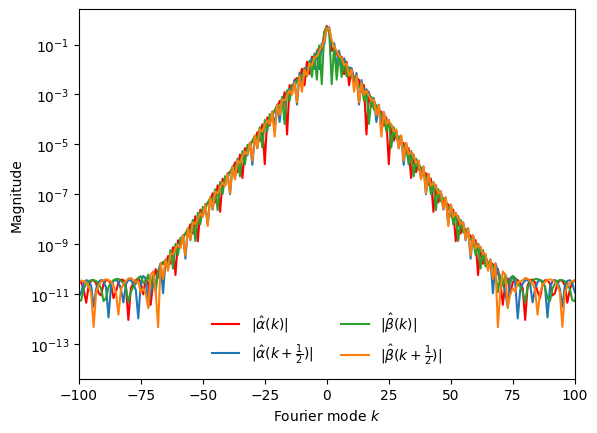
\includegraphics[width=0.3\linewidth]{b6r30eta10.png}
    (b)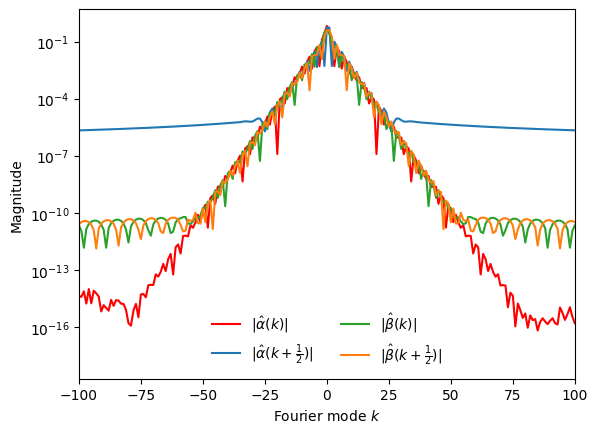
\includegraphics[width=0.3\linewidth]{b6r8eta10.png}
    (c)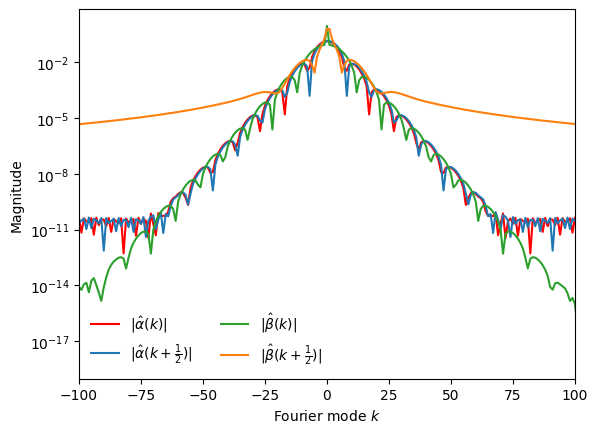
\includegraphics[width=0.3\linewidth]{b1r30eta10.png}
    \caption{Fourier magnitude spectra of the window functions $\hat \alpha(x)$ and $\hat\beta (x)$ sampled on-grid and with a half-grid shift, for (a) $b=6$, $r=30$, $\eta=10$, (b) $b=6$, $r=8$, $\eta=10$, and (c) $b=1$, $r=30$, $\eta=10$.  In each case the spectra exhibit exponential decay near the origin; for the off-grid samples, this eventually crosses over to a algebraic tail. For large enough $r$ and $b$ this crossover point occurs after the machine precision causes a plateau at approximately $10^{-10}$ on most plots.}
    \label{fig:plotwindows}
\end{figure}
\begin{figure}[htbp]
    \centering
    (a)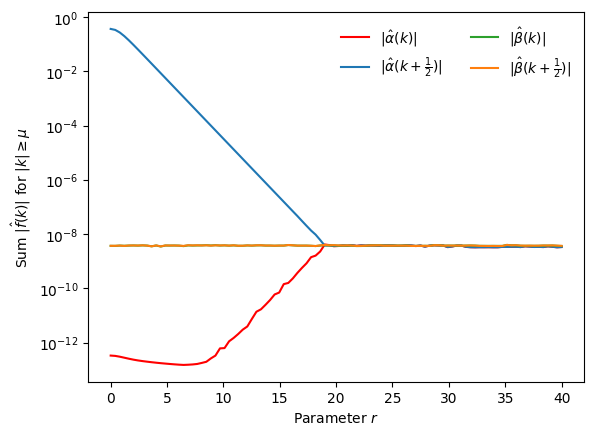
\includegraphics[width=0.3\linewidth]{scalingwithrb6eta10.png}
    (b)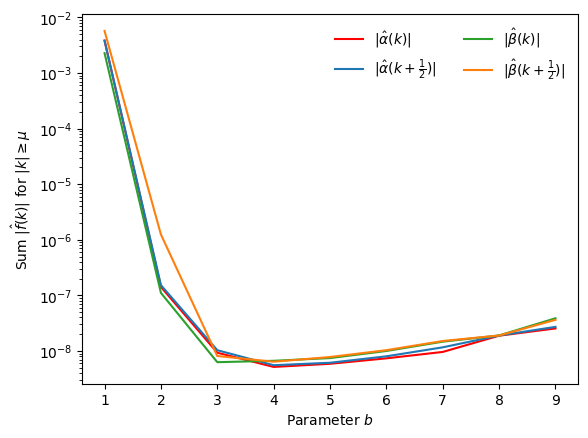
\includegraphics[width=0.3\linewidth]{scalingwithbr1000eta10.png}
    (c)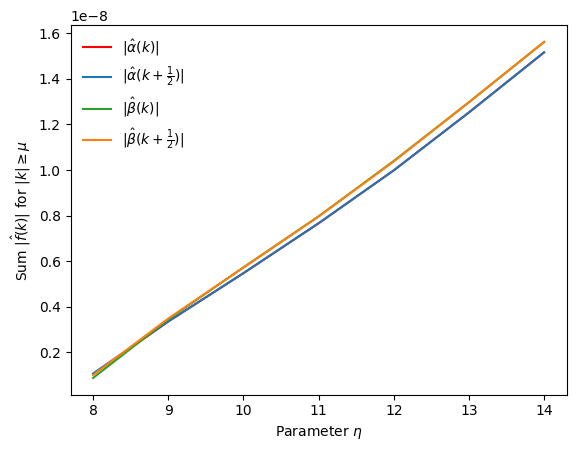
\includegraphics[width=0.3\linewidth]{scalingwithetab6r30.png}
    \caption{Scaling of the $l^1$ norm of Fourier-spectrum magnitude for modes larger than $\mu=100$ for the window functions $\hat \alpha(x)$ and $\hat\beta(x)$, sampled on-grid and with a half-grid shift. (a) Scaling with $r$ for fixed $b=6$ and $\eta=10$; (b) scaling with $b$ for fixed $r=1000$ and $\eta=10$; (c) scaling with $\eta$ for fixed $b=6$ and $r=30$.}
    \label{fig:scaling}
\end{figure}
\begin{figure}[htbp]
    \centering
    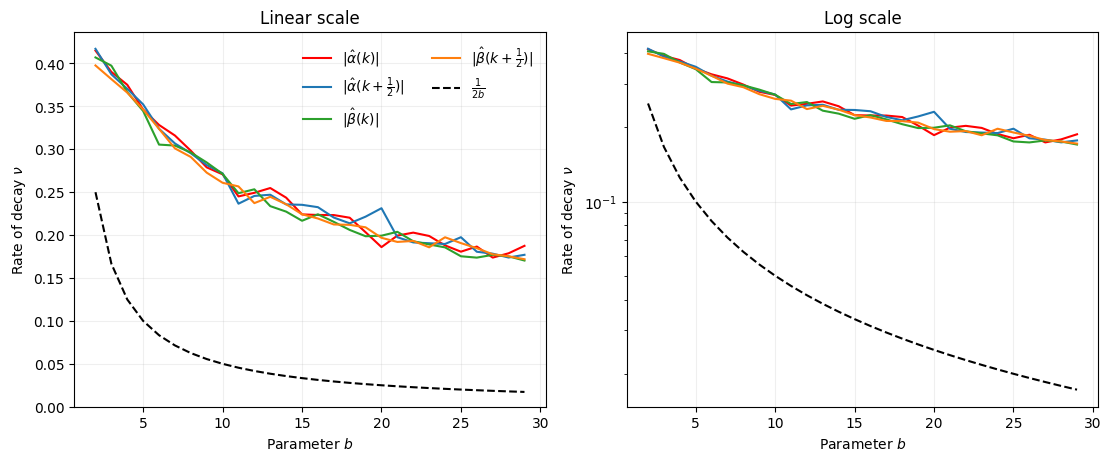
\includegraphics[width=0.75\linewidth]{nur30eta10.png}
    \caption{Scaling of the exponential decay rate $\nu$ of the Fourier-spectrum magnitude with $b$, for fixed $r=30$ and $\eta=10$. The rate is calculated by fitting a line to the log-magnitude spectrum for modes between 0 and 50. Increasing $b$ decreases the rate of exponential decay. It is clear from these plots that the lower bound on $\nu$ we derived is loose.}
    \label{fig:exponent}
\end{figure}
\begin{figure}[htbp]
    \centering
    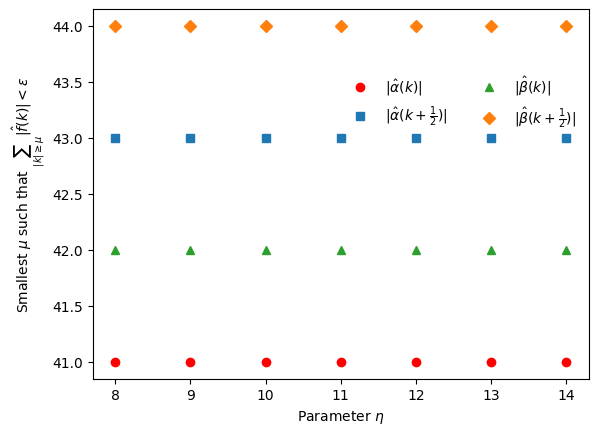
\includegraphics[width=0.4\linewidth]{scalingmuwithetab6r30.png}
    \caption{Smallest bandwidth $\mu$ required to ensure $\sum_{|k|\geq \mu}|f(k)|\leq \epsilon$ plotted against the number of ancilla qubits $\eta$ for $\epsilon = 10^{-6}$, $b=6$, and $r=30$. As expected the smallest bandwidth required for a given $\epsilon$ is independent of $\eta$ for large $r$ and $b$ over the plotted range. }
    \label{fig:scalingmu}
\end{figure}
% \begin{figure}
%     \centering
%     (a)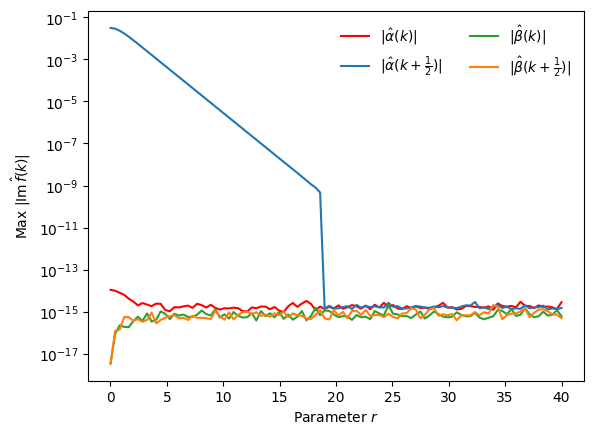
\includegraphics[width=0.4\linewidth]{imscalingwithrb6eta10.png}
%     (b)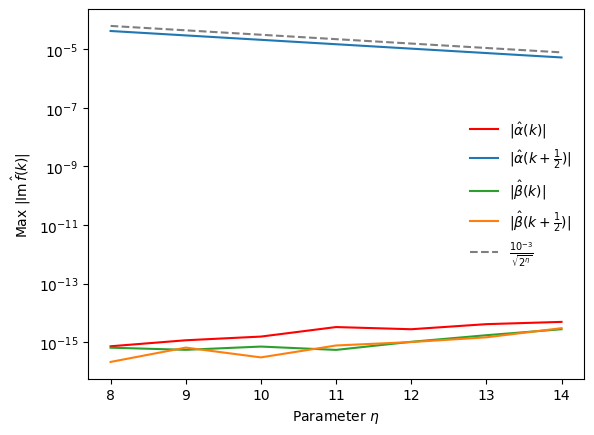
\includegraphics[width=0.4\linewidth]{scalingimwithetab6r6.png}
%     \caption{Scaling of the maximum imaginary part of the Fourier spectra of the window functions $\hat \alpha(x)$ and $\hat\beta(x)$, sampled on-grid and with a half-grid shift. (a) Scaling with $r$ for fixed $b=6$ and $\eta=10$; (b) scaling with $\eta$ for fixed $b=6$ and $r=8$.}
%     \label{fig:imag}
% \end{figure}
\pagebreak

\section{Proofs of Lemmas}
\label{section:appendixTrunc}
\begin{lemma*}[\ref{lemma:0}]
% \label{lemma:0}
    Define $\widetilde{\text{BSI-QPE}}$ as given by:
    \begin{equation}
       \widetilde{\text{BSI-QPE}}=\sum_j \sum_{p,q} \tilde G^{pq}_j \otimes \ket{p}\bra{q} \otimes \ket{\psi_j}\bra{\psi_j}
    \end{equation}
    where 
    \begin{equation}
        \tilde G^{pq}_j = \begin{pmatrix}
        (-1)^{q-p}\tilde\alpha(q-p+\frac{N}{2\pi}E_jt) & \tilde\beta(q-p+\frac{N}{2\pi}E_jt)\\
        -\tilde\beta (q-p-\frac{N}{2\pi}E_jt) & (-1)^{q-p}\tilde\alpha(q-p-\frac{N}{2\pi}E_jt)
    \end{pmatrix}
    \end{equation}
    with $\tilde\alpha(x)=\hat\alpha(x)$, $\tilde\beta(x)=\hat\beta(x)$ for $|x|_{N}\leq\mu$ and zero otherwise, then,  
    \begin{equation}
        \|\widetilde{\text{BSI-QPE}}-\text{BSI-QPE}\| \leq 2\epsilon_{\Delta}= O\left(\frac{1}{\nu}e^{-\nu \mu}\right)
    \end{equation}
    where $\epsilon_{\Delta}$ is defined in \eqref{eq:decomposealpha3}.
\end{lemma*}
\begin{proof}
    As both operators are block diagonal in the Hamiltonian eigenbasis, we will have the operator norm given by the maximum over $j$:
    \begin{equation}
        \|\widetilde{\text{BSI-QPE}}-\text{BSI-QPE}\| = \max_j 
        \left\|\sum_{p,q}(\tilde G^{pq}_j - G^{pq}_j) \otimes \ket{p}\bra{q}\right\|
    \end{equation}
    As $\|U-V\| \leq \sqrt{\|U-V\|_{1\to1}\|U-V\|_{\infty\to\infty}}$ we can bound the spectral norm by bounding the $\|\cdot\|_{1\to1}$ (maximum absolute column sum) and $\|\cdot\|_{\infty\to\infty}$ (maximum absolute row sum) operator norms. First the $\|\cdot\|_{1\to1}$  operator norm:
    \begin{multline}
         \left\|\sum_{p,q}(\tilde G^{pq}_j - G^{pq}_j) \otimes \ket{p}\bra{q}\right\|_{1\to1} = \max_q \max\bigg(\sum_{p}|\tilde\alpha(q-p+\frac{N}{2\pi}E_jt)-\hat\alpha(q-p+\frac{N}{2\pi}E_jt)|+\\|\tilde\beta (q-p-\frac{N}{2\pi}E_jt)-\hat\beta (q-p-\frac{N}{2\pi}E_jt)|, \sum_{p}|\tilde\beta(q-p+\frac{N}{2\pi}E_jt)-\hat\beta(q-p+\frac{N}{2\pi}E_jt)|+\\|\tilde\alpha (q-p-\frac{N}{2\pi}E_jt)-\hat\alpha (q-p-\frac{N}{2\pi}E_jt)|\bigg)
    \end{multline}
    which simplifies to:
    \begin{multline}
         \left\|\sum_{p,q}(\tilde G^{pq}_j - G^{pq}_j) \otimes \ket{p}\bra{q}\right\|_{1\to1} = \max_q\max\bigg(\sum_{\substack{p\\|q-p+\frac{N}{2\pi}E_jt|_{N}>\mu}}|\hat\alpha(q-p+\frac{N}{2\pi}E_jt)|+\sum_{\substack{p\\|q-p-\frac{N}{2\pi}E_jt|_{N}>\mu}}|\hat\beta (q-p-\frac{N}{2\pi}E_jt)|,\\
         \sum_{\substack{p\\|q-p+\frac{N}{2\pi}E_jt|_{N}>\mu}}|\hat\beta(q-p+\frac{N}{2\pi}E_jt)|+\sum_{\substack{p\\|q-p-\frac{N}{2\pi}E_jt|_{N}>\mu}}|\hat\alpha (q-p-\frac{N}{2\pi}E_jt)|\bigg)
    \end{multline}
    Therefore, using \eqref{eq:scaling} and \eqref{eq:decomposealpha3}  we can see:
    \begin{equation}
        \left\|\sum_{p,q}(\tilde G^{pq}_j - G^{pq}_j) \otimes \ket{p}\bra{q}\right\|_{1\to1} \leq 2\epsilon_{\Delta} = O(\frac{1}{\nu}e^{-\nu \mu})
    \end{equation}
    A similar process gives us:
    \begin{equation}
        \left\|\sum_{p,q}(\tilde G^{pq}_j - G^{pq}_j) \otimes \ket{p}\bra{q}\right\|_{\infty\to\infty} \leq 2\epsilon_{\Delta} =O(\frac{1}{\nu}e^{-\nu \mu})
    \end{equation}
    Thus,
    \begin{equation}
        \|\widetilde{\text{BSI-QPE}}-\text{BSI-QPE}\| \leq 2\epsilon_{\Delta} = O\left(\frac{1}{\nu}e^{-\nu \mu}\right)
    \end{equation}
\end{proof}
\begin{lemma*}[\ref{lemma:3}]
% \label{lemma:3}
Let $\{D_s\}_{s\in S}$ be mutually orthogonal projectors satisfying $\sum_{s\in S} D_s \leq \mathbb{I}$. Given unitaries $U$ and $V$, define the measurement $K_s = U^{\dagger}D_s V$ and CP map $\mathcal{K}[\rho] = \sum_{s \in S} K_s\rho K_s^{\dagger}$. Further, given operators $\tilde U, \tilde V$, define approximate measurement operators $\tilde K_s = \tilde U^{\dagger}D_s \tilde V$ and the approximate map $\tilde{\mathcal{K}}[\rho] = \sum_{s \in S} \tilde K_s\rho \tilde K_s^{\dagger}$. If $\|U-\tilde U\| \leq \epsilon<\frac14$ and $\|V-\tilde V\| \leq \epsilon<\frac14$, then 
\begin{equation}
    \|\mathcal{K} - \tilde{\mathcal{K}}\|_{\diamond} \leq 6\epsilon
\end{equation}
\end{lemma*}
\begin{proof}
First, consider:
\begin{align}
    \mathcal{K}[\rho] - \tilde{\mathcal{K}}[\rho] &= \sum_{s \in S} K_s\rho K_s^{\dagger} - \tilde K_s\rho \tilde K_s^{\dagger} \\
    &= \sum_{s \in S} (K_s-\tilde K_s)\rho K_s^{\dagger} +\tilde K_s\rho (K_s^{\dagger}- \tilde K_s^{\dagger}) \label{eq:ksUdiff}
\end{align}
For $\Phi[\rho]=\sum_sR_{1,s}\rho R_{2,s}^\dagger$, define $V_i=\sum_s\ket{s}_S\otimes R_{i,s}$ for $i \in \{1,2\}$. Therefore, we can write $\Phi[\rho] = \operatorname{Tr}_S[V_1\rho V_2^{\dagger}]$. For any ancillary system $A$, the Schatten trace-norm duality gives:
\begin{align}
    \|(\Phi\otimes\operatorname{id}_A)[\rho]\|_* &= \sup_{\|X\|\leq 1} | \operatorname{Tr}[X (\operatorname{Tr}_S[(V_1\otimes \mathbb{I}_A) \rho (V_2^{\dagger}\otimes \mathbb{I}_A)]|\\
    &=\sup_{\|X\|\leq 1} | \operatorname{Tr}[(\mathbb{I}_S \otimes X ) (V_1\otimes \mathbb{I}_A) \rho (V_2^{\dagger}\otimes \mathbb{I}_A)]|\\
    &\leq\sup_{\|X\|\leq 1} \| (V_2^{\dagger}\otimes \mathbb{I}_A)(\mathbb{I}_S \otimes X ) (V_1\otimes \mathbb{I}_A) \rho \|_*\\
    &\leq \sup_{\|X\|\leq 1} \| V_2^{\dagger}\|\|X\| \|V_1\| \| \rho \|_* = \|V_1\|\| V_2\| \| \rho \|_*
\end{align}
where the last inequality comes from the generalised H\"older inequality of schatten norms. As $\|\Phi\|_{\diamond} = \sup_A\sup_{\|\rho\|_*\leq 1}\|(\Phi\otimes\operatorname{id}_A)[\rho]\|_*$ and
\(V_i^\dagger V_i=\sum_sR_{i,s}^\dagger R_{i,s}\), we have
\begin{equation}
\|\Phi\|_\diamond
\leq
\left\|\sum_{s\in S}R_{1,s}^\dagger R_{1,s}\right\|^{1/2}
\left\|\sum_{s\in S}R_{2,s}^\dagger R_{2,s}\right\|^{1/2}.
\end{equation}
Applying the above bound to Eq.~\eqref{eq:ksUdiff}
gives
\begin{equation}
\|\mathcal{K}-\tilde{\mathcal{K}}\|_\diamond
\leq
\left\|\sum_{s\in S}(K_s^\dagger - \tilde K_s^\dagger)(K_s - \tilde K_s)\right\|^{1/2}
\left(
\left\|\sum_{s\in S}K_s^\dagger K_s\right\|^{1/2}
+
\left\|\sum_{s\in S}\tilde K_s^\dagger\tilde K_s\right\|^{1/2}
\right).
\label{eq:row-column-bound}
\end{equation}
Let us evaluate the terms in this expression. First, we have
\begin{equation}
     \left\|\sum_{s\in S} K_s^{\dagger}  K_s \right\| = \left\|\sum_{s\in S}  V^{\dagger}D_sV \right\| \leq  \left\|V^{\dagger} V\right\| = 1
\end{equation}

Second, we have
\begin{align}
    \left\|\sum_{s\in S}\tilde K_s^{\dagger} \tilde K_s \right\|^{\frac{1}{2}} &= \left\|\sum_{s\in S} \tilde V^{\dagger} D_s \tilde U\tilde U^{\dagger}  D_s \tilde V\right\|^{\frac{1}{2}} \\
     &\leq \|\tilde U\|\left\|\sum_{s\in S} \tilde V^{\dagger} D_s  \tilde V\right\|^{\frac{1}{2}}\\
     &\leq \|\tilde U\| \|\tilde V^{\dagger}  \tilde V\|^{\frac{1}{2}}= \|\tilde U\|\|\tilde V\| \leq (1+\epsilon)^2\\
\end{align}
Finally let us consider:
\begin{align}
    K_s-\tilde K_s &= U^{\dagger}  D_s V-\tilde U^{\dagger}  D_s \tilde V\\
    &=  (U-\tilde U)^{\dagger}  D_s V+\tilde U^{\dagger}  D_s (V-\tilde V)\\
\end{align}
Let us define $E_U = U - \tilde U$, then:
\begin{align}
    \left\|\sum_{s\in S}(K_s^\dagger - \tilde K_s^\dagger)(K_s - \tilde K_s)\right\|^{\frac{1}{2}}&= \left\| \sum_{s \in S}\ket{s} \otimes ( E_U^{\dagger}  D_s V+\tilde U^{\dagger}  D_sE_V)\right\|\\
    &\leq  \left\| \sum_{s \in S} \ket{s} \otimes E_U^{\dagger}  D_s V \right\| + \left\| \sum_{s \in S} \ket{s} \otimes \tilde U^{\dagger}  D_sE_V\right\|\\
    &\leq \left\| \sum_{s \in S}  V^{\dagger}  D_sE_UE_U^{\dagger} D_s  V\right\|^{\frac{1}{2}} +  \left\| \sum_{s \in S} E_V^{\dagger}  D_s \tilde U \tilde U^{\dagger} D_s E_V \right\|^{\frac{1}{2}}\\
    &\leq \|E_U\| + \|E_V\|\|\tilde U\| \leq \epsilon(2+\epsilon)
\end{align}

Therefore,
\begin{equation}
    \|\mathcal{K} - \tilde{\mathcal{K}}\|_{\diamond} \leq \epsilon(2+\epsilon)(1+(1+\epsilon)^2)
\end{equation}
Using $\epsilon<\frac14$, we obtain $\|\mathcal{K} - \tilde {\mathcal{K}}\|_{\diamond} \leq 6\epsilon$.
\end{proof}
\begin{lemma*}[\ref{lemma:composition}]
Let $\mathcal{M}_1, \ldots, \mathcal{M}_k$ be completely positive trace-non-increasing maps and let $\tilde{\mathcal{M}}_1, \ldots, \tilde{\mathcal{M}}_k$ be completely positive maps with $\|\mathcal{M}_i - \tilde{\mathcal{M}}_i\|_{\diamond} \leq \varepsilon$ for all $i$. Then
\begin{equation}
    \|\mathcal{M}_k \circ \cdots \circ \mathcal{M}_1 - \tilde{\mathcal{M}}_k \circ \cdots \circ \tilde{\mathcal{M}}_1\|_{\diamond} \leq (1+\varepsilon)^k - 1 \leq e k \varepsilon,
\end{equation}
the last inequality holding whenever $k\varepsilon \leq 1$. More generally, if instead $\|\mathcal{M}_i\|_{\diamond}, \|\tilde{\mathcal{M}}_i\|_{\diamond} \leq c$ for some $c \geq 1$ and $\|\mathcal{M}_i - \tilde{\mathcal{M}}_i\|_{\diamond} \leq \varepsilon_i$, without assuming the $\mathcal{M}_i$ are trace-non-increasing, then
\begin{equation}
    \|\mathcal{M}_k \circ \cdots \circ \mathcal{M}_1 - \tilde{\mathcal{M}}_k \circ \cdots \circ \tilde{\mathcal{M}}_1\|_{\diamond} \leq c^{k-1}\sum_{i=1}^{k}\varepsilon_i .
\end{equation}
\end{lemma*}
\begin{proof}
    Writing the difference as a telescoping sum,
\begin{equation}
    \mathcal{M}_k \circ \cdots \circ \mathcal{M}_1 - \tilde{\mathcal{M}}_k \circ \cdots \circ \tilde{\mathcal{M}}_1 = \sum_{i=1}^{k} \mathcal{M}_k \circ \cdots \circ \mathcal{M}_{i+1} \circ (\mathcal{M}_i - \tilde{\mathcal{M}}_i) \circ \tilde{\mathcal{M}}_{i-1} \circ \cdots \circ \tilde{\mathcal{M}}_1,
\end{equation}
and using submultiplicativity of the diamond norm together with $\|\mathcal{M}_i\|_{\diamond} \leq 1$ (completely positive trace-non-increasing) and $\|\tilde{\mathcal{M}}_i\|_{\diamond} \leq \|\mathcal{M}_i\|_{\diamond} + \varepsilon \leq 1 + \varepsilon$, we obtain
\begin{equation}
    \|\mathcal{M}_k \circ \cdots \circ \mathcal{M}_1 - \tilde{\mathcal{M}}_k \circ \cdots \circ \tilde{\mathcal{M}}_1\|_{\diamond} \leq \sum_{i=1}^{k}\varepsilon(1+\varepsilon)^{i-1} = (1+\varepsilon)^k - 1.
\end{equation}
For $k\varepsilon \leq 1$ we have $(1+\varepsilon)^k \leq e^{k\varepsilon} \leq 1 + e k\varepsilon$, giving the final inequality. For the general statement, the $i$-th term of the same telescoping sum has diamond norm at most $c^{k-i}\,\varepsilon_i\,c^{i-1} = c^{k-1}\varepsilon_i$.
\end{proof}
\begin{lemma*}[\ref{lemma:summed-history-reversal}]
For $n\geq1$, let $\{x_i\}_{i=1}^{n+1}$ and $\{y_i\}_{i=1}^{n+1}$ denote
the compound labels
\begin{equation*}
    y_i=(b_{2n+3-2i},d_{n+2-i}),\qquad x_i=(c_{2n+3-2i},d'_{n+2-i}),
\end{equation*}
with $a,e$ fixed.  Choose $\theta_x\in[0,\pi/2]$ so that
\begin{equation*}
    W_x=W_{bd}=\begin{pmatrix}
                \sqrt{1 - f_{abde}} & \sqrt{f_{abde}}\\
       \sqrt{f_{abde}} & -\sqrt{1 - f_{abde}}
    \end{pmatrix}= \begin{pmatrix}\cos\theta_x&\sin\theta_x\\
    \sin\theta_x&-\cos\theta_x\end{pmatrix},
\end{equation*}
and set $\Delta_i=\theta_{y_i}-\theta_{x_i}$.  Then
\begin{equation}
    \bar g^{ae}(\{b\},\{c\},\{d\},\{d'\})
    =\frac12\cos\Delta_1\cos\Delta_{n+1}
      \prod_{i=1}^{n}\cos(\Delta_i-\Delta_{i+1}).
\end{equation}
Consequently,
\begin{equation}
    \bar g^{ae}(\{b\},\{c\},\{d\},\{d'\})
    =\bar g^{ae}(\{c\}^R,\{b\}^R,\{d'\}^R,\{d\}^R).
    \label{eq:PRR}
\end{equation}
\end{lemma*}
\begin{proof}
Put $\ket{v_s(x)}=W_x\ket{s}$, so
$R_s^x=\ket{v_s(x)}\bra{v_s(x)}$. Therefore, we can rewrite $\bar g^{ae}$ for $n\geq 1$ \eqref{eq:gbar-definition} as:
\begin{multline}
    \frac{1}{2}\sum_{s_0,\ldots,s_n} \braket{0|v_{s_0}(x_1)}\braket{v_{s_0}(x_1)|v_{s_1}(x_2)}\ldots \braket{v_{s_{n-1}}(x_n)|v_{s_n}(x_{n+1})}\braket{v_{s_n}(x_{n+1})|v_{s_n}(y_{n+1})}\\\braket{v_{s_n}(y_{n+1})|v_{s_{n-1}}(y_n)}\ldots\braket{v_{s_1}(y_2)|v_{s_0}(y_1)}\braket{v_{s_0}(y_1)|0}
\end{multline}
We can reorder this to get:
\begin{multline}
    \frac{1}{2}\sum_{s_0,\ldots,s_n} \braket{0|v_{s_0}(x_1)}\braket{v_{s_0}(y_1)|0}\braket{v_{s_0}(x_1)|v_{s_1}(x_2)}\braket{v_{s_1}(y_2)|v_{s_0}(y_1)}\ldots\\ \braket{v_{s_{n-1}}(x_{n})|v_{s_{n}}(x_{n+1})}\braket{v_{s_{n}}(y_{n+1})|v_{s_{n-1}}(y_{n})}\braket{v_{s_{n}}(x_{n+1})|v_{s_{n}}(y_{n+1})}
\end{multline}
For consecutive labels define
the two-state transfer matrix
\begin{equation*}
    (T_i)_{uv}=\braket{v_u(x_i)|v_v(x_{i+1})}
    \braket{v_v(y_{i+1})|v_u(y_i)}.
\end{equation*}
Therefore, we can rewrite $\bar g$ as:
\begin{equation}
   \frac{1}{2}\sum_{s_0,\ldots,s_n} h_{s_0}(T_1)_{s_0s_1}(T_2)_{s_1s_2}\ldots (T_n)_{s_{n-1}s_{n}} c_{s_n}
\end{equation}
where $h_s = \braket{0|v_{s}(x_1)}\braket{v_{s}(y_1)|0}$ and $c_s =\braket{v_{s}(x_{n+1})|v_{s}(y_{n+1})}$. Hence, we can write $\bar g$ as simple matrix multiplication:
\begin{equation}
    \bar g(\{b\},\{c\},\{d\},\{d'\}) = \frac{1}{2}hT_1T_2T_3\ldots T_nc
\end{equation}
As $W_xW_y = \begin{pmatrix}
    \cos (\theta_x - \theta_y) & - \sin (\theta_x - \theta_y)\\
     \sin (\theta_x - \theta_y) & \cos (\theta_x - \theta_y)
\end{pmatrix}$ we have:
\begin{align}
    (T_i)_{u v} &=  \begin{pmatrix}
    \cos (\theta_{x_i} - \theta_{x_{i+1}}) & - \sin (\theta_{x_i} - \theta_{x_{i+1}})\\
     \sin (\theta_{x_i} - \theta_{x_{i+1}}) & \cos (\theta_{x_i} - \theta_{x_{i+1}})
\end{pmatrix}_{uv} \begin{pmatrix}
    \cos (\theta_{y_{i+1}} - \theta_{y_{i}}) & - \sin (\theta_{y_{i+1}} - \theta_{y_{i}})\\
     \sin (\theta_{y_{i+1}} - \theta_{y_{i}}) & \cos (\theta_{y_{i+1}} - \theta_{y_{i}}) 
\end{pmatrix}_{vu}\\
&=\begin{pmatrix}
    \cos (\theta_{x_i} - \theta_{x_{i+1}})\cos (\theta_{y_{i+1}} - \theta_{y_{i}}) & - \sin (\theta_{x_i} - \theta_{x_{i+1}})\sin (\theta_{y_{i+1}} - \theta_{y_{i}})\\
     -\sin (\theta_{x_i} - \theta_{x_{i+1}})\sin (\theta_{y_{i+1}} - \theta_{y_{i}}) & \cos (\theta_{x_i} - \theta_{x_{i+1}}) \cos (\theta_{y_{i+1}} - \theta_{y_{i}}) 
\end{pmatrix}_{uv}\\
&=  \cos (\theta_{y_i} - \theta_{y_{i+1}})\cos (\theta_{x_{i}} - \theta_{x_{i+1}}) \mathbb{I}_{uv} + \sin (\theta_{y_i} - \theta_{y_{i+1}})\sin (\theta_{x_{i}} - \theta_{x_{i+1}}) X_{uv}
\end{align}
We can also clearly see that $c = \cos (\theta_{x_{n+1}} -\theta_{y_{n+1}}) \begin{pmatrix}
    1\\1
\end{pmatrix} =  \cos(\Delta_{n+1})\begin{pmatrix}
    1\\1
\end{pmatrix} $, and we have that $\begin{pmatrix}
    1\\1
\end{pmatrix}$ is an eigenvector of all $T_i$ as $T_i = \alpha_i \mathbb{I} + \beta_i X$. The corresponding eigenvalue for each $T_i$ is given by:
\begin{align}
    \alpha_i+\beta_i&=\cos (\theta_{y_i} - \theta_{y_{i+1}})\cos (\theta_{x_{i}} - \theta_{x_{i+1}}) + \sin (\theta_{y_i} - \theta_{y_{i+1}})\sin (\theta_{x_{i}} - \theta_{x_{i+1}}) \\
    &= \cos(\theta_{y_i} - \theta_{y_{i+1}} - (\theta_{x_{i}} - \theta_{x_{i+1}}))\\
    &= \cos\!\left(\theta_{y_i} - \theta_{x_i} - (\theta_{y_{i+1}} - \theta_{x_{i+1}})\right)\\
    &= \cos(\Delta_i - \Delta_{i+1})
\end{align}
Therefore, $T_1T_2T_3\ldots T_nc = \cos(\Delta_{n+1})\prod_{i=1}^{n}\cos(\Delta_i - \Delta_{i+1})\begin{pmatrix}
    1\\1
\end{pmatrix}$. As $h = \begin{pmatrix}
    \cos(\theta_{x_1})\cos(\theta_{y_1})& \sin(\theta_{x_1})\sin(\theta_{y_1})
\end{pmatrix}$, we have $h\begin{pmatrix}
    1\\1
\end{pmatrix}= \cos(\theta_{x_1})\cos(\theta_{y_1}) + \sin(\theta_{x_1})\sin(\theta_{y_1}) = \cos(\theta_{x_1}-\theta_{y_1}) = \cos(\Delta_1)$. Therefore,
\begin{equation}
    \bar g(\{b\},\{c\},\{d\},\{d'\}) =\frac{1}{2}\cos(\Delta_1)\cos(\Delta_{n+1})\prod_{i=1}^{n}\cos(\Delta_i - \Delta_{i+1})
\end{equation}
  Exchanging $b,d'$ ($x$) with $c,d$ ($y$) maps $\Delta_i\mapsto-\Delta_i$, and $\bar g$ is preserved because cosine is even. Reversing $\{b\}$, $\{c\}$, $\{d\}$ and $\{d'\}$ maps $\Delta_i\mapsto\Delta_{n+2-i}$. As $\frac{1}{2}\cos(\Delta_{n+1})\cos(\Delta_{1})\prod_{i=1}^{n}\cos(\Delta_{n+2-i} - \Delta_{n+1-i}) = \frac{1}{2}\cos(\Delta_1)\cos(\Delta_{n+1})\prod_{i=1}^{n}\cos(\Delta_i - \Delta_{i+1})$, the quantity $\bar g$ is preserved and Eq.~\eqref{eq:PRR} holds.
\end{proof}
\begin{lemma*}[\ref{lemma:wdrift} $W$-drift]
% \label{lemma:wdrift}
For all $a,b,d,e$ and all $|z|_{N} \leq (4n+6)\mu$,
\begin{equation}
    \|W^F_{a-z,b-z,de} - W^F_{abde}\| \leq 2\sqrt{\beta\frac{6\pi}{Nt}}\sqrt{(4n+6)\mu}.
\end{equation}
\end{lemma*}
\begin{proof}
    By definition we have
\begin{equation}
     W^F_{a-z,b-z,de} = \begin{pmatrix}
        \sqrt{1 - F(\kappa_{a-z,b-z,de})} & \sqrt{F(\kappa_{a-z,b-z,de})}\\
       \sqrt{F(\kappa_{a-z,b-z,de})} & -\sqrt{1 - F(\kappa_{a-z,b-z,de})}
    \end{pmatrix}
\end{equation}
where:
\begin{equation}
    F(\kappa) = \begin{cases}1& \text{ for }  -\frac{N}{2} \leq \kappa <  -\frac{3N}{8}\\
        \min(1,e^{-\beta \frac{2\pi}{Nt} \kappa}) & \text{ for } |\kappa|\leq \frac{3N}{8}\\
        e^{-\beta\frac{3\pi}{4t}} + \frac{1- e^{-\beta\frac{3\pi}{4t}}}{\frac{N}{8}}(\kappa - \frac{3N}{8}) & \text{ for }  \frac{3N}{8} < \kappa <  \frac{N}{2}
    \end{cases}
\end{equation}
and
\begin{equation}
    \kappa_{a-z,b-z,de} \equiv (-1)^d(b-z) - (-1)^e(a-z) \mod N \text{ for } -\frac{N}{2} \leq \kappa_{a-z,b-z,de} < \frac{N}{2}
\end{equation}
As $|z|_{N} \leq (4n+6)\mu< \frac{N}{8}$  we have:
\begin{equation}
    |\kappa_{a-z,b-z,de} - \kappa_{abde}|_{N} \leq 2(4n+6)\mu
\end{equation}
The function $F$ is continuous and $N$-periodic, so its Lipschitz constant with respect to the circular distance $|\cdot|_{N}$ is given by its largest gradient. For $|\kappa|\leq \frac{3N}{8}$ the largest gradient is given by $\frac{2\pi\beta}{Nt}$, whereas for $ \frac{3N}{8} < \kappa <  \frac{N}{2}$ the gradient is given by $\frac{1- e^{-\beta\frac{3\pi}{4t}}}{\frac{N}{8}} \leq \frac{6\pi\beta}{Nt}$. Therefore,
\begin{equation}
     |F(\kappa)-F(\kappa')|\leq \frac{6\pi\beta}{Nt}|\kappa - \kappa'|_{N} \qquad \forall \quad \kappa, \kappa'
\end{equation}
Hence,
\begin{equation}
    |F(\kappa_{a-z,b-z,de})-F(\kappa_{abde})|\leq 12(4n+6)\frac{\pi\mu\beta}{Nt}
\end{equation}
We have
\begin{equation}
    W^F_{a-z,b-z,de}-W^F_{abde}=\begin{pmatrix} p & q\\ q & -p\end{pmatrix}
\end{equation}
where $p=\sqrt{1-F(\kappa_{a-z,b-z,de})}-\sqrt{1-F(\kappa_{abde})}$ and $q=\sqrt{F(\kappa_{a-z,b-z,de})}-\sqrt{F(\kappa_{abde})}$. This matrix is real symmetric and squares to $(p^2+q^2)\mathbb{I}$, so its operator norm is $\sqrt{p^2+q^2}$. Since $|\sqrt{x}-\sqrt{y}|\le\sqrt{|x-y|}$ for all $x,y\ge 0$, we have $|p|\leq \sqrt{12(4n+6)\frac{\pi\mu\beta}{Nt}}$ and $|q|\leq \sqrt{12(4n+6)\frac{\pi\mu\beta}{Nt}}$. Therefore
\begin{equation}
    \|W^F_{a-z,b-z,de}-W^F_{abde}\|\le\sqrt{24(4n+6)\frac{\pi\mu\beta}{Nt}}
    =2\sqrt{\beta\frac{6\pi}{Nt}}\sqrt{(4n+6)\mu}
\end{equation}
\end{proof}
\clearpage
\end{document}